\documentclass[11pt]{article}
\usepackage[margin=1in]{geometry}
\usepackage{graphicx}
\usepackage{booktabs}
\usepackage{hyperref}
\usepackage{amsmath}
\usepackage{amssymb}
\usepackage{float}
\usepackage{array}
\usepackage{tabularx}
\usepackage{longtable}
\usepackage{pdflscape}
\usepackage{enumitem}
\setlength{\emergencystretch}{2em}

\title{A morphology-matched forward-readout protocol for SPARC rotation curves}
\author{Jozsef Olcsak}
\date{Last revised: 30 August 2026}

\begin{document}
\maketitle

\begin{abstract}
This paper tests whether residual-blind morphology/readout information can
choose a rotation-curve readout family before the residuals are inspected.
Standard rotation-curve tests
usually compare baryonic Newtonian predictions with universal or weakly
morphology-dependent correction laws.  This paper develops a different,
claim-bounded protocol: before scoring a rotation curve, assign a
residual-blind morphology/readout state, select the corresponding readout
family, freeze source-side scales and amplitudes where possible, and compare the
matched family against wrong-family, shuffled-label, Newtonian, MOND-like, RAR,
and fixed predecessor-readout controls.  The protocol is motivated by three observations
that are made self-contained here: external structural disturbance can correlate
with residual structure; residual-shape diagnostics are useful but inverse; and
a forward test must choose the readout family without using endpoint residuals.
Using SPARC rotation curves as the common numerical arena, the accompanying reproducibility code
finds a retrospective internal label--formula compatibility signal: a source-native
readout-formula preflight beats wrong readout-formula families in \(0.886\) of
the 44 holdout galaxies.  For the shuffled-label null, the mean
matched-minus-wrong statistic gives \(p\simeq0.002\) in the 1000-shuffle
endpoint run, while the beat-fraction statistic is reported separately below.
The matched-versus-wrong signal is preserved in a Newtonian-carrier
amplitude-freeze stress test, supporting carrier robustness but not baseline
superiority.
However, a later cross-fitted audit of the same 45-galaxy Paper 1--3 label
packet finds no stable projection-contrast increment after endpoint-residual-free
observability/baryonic covariates and MOND/RAR-common residual structure are
supplied.  In addition, a source-frozen seven-galaxy EDGE--CALIFA matched-tracer
stress test fails its predeclared external morphology-alignment gate
(mean \(D=-0.0587\), exact one-sided \(p=0.6016\), four of seven positive).
Further public-data routes do not reverse that verdict: a prospective
14-galaxy LITTLE THINGS replay gives only mixed one-family transfer; low-order
PHANGS CO--H\(\alpha\) structure either obeys the morphology-orthogonal null or
fails source-label specificity; and a higher-dimensional PHANGS confirmatory
packet stops at its predeclared spatial-support gate without releasing a
score.  A robust one-galaxy NGC4254 \(m=2\) source coordinate survives internal
source controls, but its terminal gain and primitive action curvature are
non-identifiable from the present source state.  Thus the internal preflight
has not transferred into conditional specificity or external confirmation.
Moreover,
the same preflight beats a fixed TPG/v6 predecessor comparator and MOND-like comparators in only \(0.477\) of
holdout galaxies each, so it is not evidence that the proposed framework
outperforms existing baselines as a population law.  A separate all-SPARC
175-galaxy morphology triage identifies 39 source-freeze candidates, 61
source/kernel precision cases, 18 morphology/subfamily review cases, and 57
control or low-quality cases.  Four inspected single-galaxy readout cases also
show encouraging matched-family behavior, but remain heterogeneous and
caveated.  An unchanged-law transfer from the strongest NGC4088 case to the
source-native outer warp of UGC08490/NGC5204 preserves a weak morphology-ordering
signal---the correct onset gives \(29.70\,{\rm km\,s^{-1}}\) RMSE versus
\(31.64\,{\rm km\,s^{-1}}\) for the wrong NGC4088 onset---but fails badly against
fixed MOND (\(8.78\,{\rm km\,s^{-1}}\)) and two-parameter halo fits
(\(1.20\)--\(1.55\,{\rm km\,s^{-1}}\)).  This is a reproducible negative result
for the present one-component universal warp-law transfer, not for morphology
information or Tau Core in general.  A second unchanged-law replication on
the source-selected warp of UGC03580/UGC3580 is stronger: the source-correct
onset gives \(38.04\,{\rm km\,s^{-1}}\) full-curve RMSE, worse than Newtonian
baryons (\(36.01\)), fixed MOND (\(27.17\)), and an earlier wrong-onset control
(\(24.56\)).  The uncapped kernel also overshoots beyond \(R_{\rm HI}\).
Together these transfers reject the present uncapped one-component law as a
universal warp-class rotation law.  An endpoint-blind follow-up replaces the
scalar UGC03580 onset proxy by a piecewise geodesic path through all published
supported tilted-ring orientations.  It reconstructs the independent
inner/outer plane angle.  The resulting defect-ratio family is bounded, but an
explicit counterfamily proves that the body alone does not select its power,
amplitude, sign, carrier, or physical occupation.  A standard fixed-inclination
projection control reaches \(1.09685\) in squared speed on the supported rings
and must be audited and, where applicable, accounted for before any Tau
attribution.  No rotation endpoint is used
or rescored in this derivation.  A later source-frozen NGC~4062
H\,\textsc{i}--H$\alpha$ endpoint is null in both resolutions and changes sign
under the alternate published velocity zero point; it is therefore a preserved
calibration-limited negative endpoint, not a Tau-specific detection or an
accepted framework-level true negative.  The analysis otherwise contains
branch-level negative controls and morphology-underdetermined weak negatives,
but no source-complete endpoint-grade true negative.  The main conclusion is therefore
methodological: morphology-matched forward readouts define a falsifiable
endpoint protocol, not a validated gravity theory.  A practical next step is a
residual-blind readout morphology catalogue that freezes source morphology,
projection, H I support, vertical structure, and morphology-trajectory/phase
observables before endpoint scoring.  The result should be read as a reproducible protocol
and internal preflight signal, not as evidence for a new gravitational law.
\end{abstract}

\section{Introduction}

The SPARC data set provides high-quality rotation curves and baryonic mass
models for 175 disk galaxies \cite{Lelli2016SPARC}.  It is a standard testbed
for Newtonian baryonic predictions, MOND-like dynamics, and empirical
radial-acceleration relations \cite{Milgrom1983MOND,McGaugh2016RAR,Li2018RARFits}.
These comparisons are usually organized around scalar acceleration laws or
globally fitted mass-to-light choices.  They are powerful precisely because they
are simple.

The comparison set in this paper has two different kinds of baselines.  The
Newtonian, MOND-like, and RAR-like references are external literature-facing
comparators.  The TPG/v6 curve, by contrast, is an internal predecessor
readout/closure comparator from the same research programme.  It is included
because it is frozen in the reproducibility package and is often a strong
smooth baseline.  It is not treated here as an independently published
reference model, and it is not used to choose or tune the morphology-matched
readout family.

The present paper asks a different question.  Suppose that some residual
structure is not described well by a universal scalar correction, but depends on
which morphology/readout state the galaxy occupies: regular disk, extended
scale-tail disk, compact finite-source system, vertical/projection-dominated
system, ring/resonance structure, warp/trajectory structure, or a mixture of such
components.  Then the relevant test is not merely whether a flexible curve can
fit a galaxy.  The test is whether the morphology-matched readout family,
chosen before endpoint scoring, performs better than wrong morphology families
and shuffled labels, and only then whether it is competitive with conventional
baselines.

The forward kernel is deliberately a terminal hypothesis. A morphology label,
a fitted rotation residual, or a successful matched-family score does not
construct a smooth parent source arrow or optical/body connection. Current
Tau Core source accounting permits such non-scalar transport only after an
independently sourced full body connection or a varying, constant-rank,
source-owned access projector has been supplied. This added boundary does not
alter the scoring problem below; it prevents a terminal success from being
reinterpreted as identification of the upstream transport mechanism.

This paper makes that test self-contained.  The framework is used only through
operational definitions.  In Tau Core terminology the intrinsic source object is
the \emph{morphological body} \(M_\tau\), while the data used here are only
projected and source-frozen handles on that body: a galaxy has a projected morphology handle
\(K_{\rm obs}\), a possibly different readout-relevant proxy
\(K_{\rm readout}\), and a family of local readout kernels that generate a
forward correction \(\delta v_K^2(R)\) or equivalent closure response.  No
external theory paper is required for the protocol.  The definitions, allowed
inputs, forbidden inputs, endpoint score, negative-result taxonomy, and
numerical status are stated below.

\subsection{Reader's roadmap}

\noindent\fbox{%
\begin{minipage}{0.94\linewidth}
\textbf{What must be accepted to read the paper:} only the operational protocol
defined here.  A reader does not need to accept a completed new gravity theory.

\textbf{What is tested:} whether a residual-blind morphology/readout label can
choose a restricted readout family that performs better than wrong families and
shuffled labels.

\textbf{What is not claimed:} population-level superiority over Newtonian,
MOND/RAR-like, or TPG/v6-like baselines; a final morphology catalogue; or a
validated gravitational theory.

\textbf{Where the evidence appears:} Section~3 defines the scoring protocol;
Section~4 defines the readout families; Section~5 gives the reproducibility and
leakage-prevention path; Section~6 reports population preflights, the
175-galaxy triage, four inspected rotation-curve cases, and the unchanged-law
UGC08490 transfer; Section~7 explains how to read failures.
\end{minipage}
}

Equations~\eqref{eq:fibre-sufficiency}--\eqref{eq:post-open-saturation} make
this taxonomy falsifiable.  A representation-level failure may motivate a
new source-only representation, but it cannot be relabeled as a body-level
success and it cannot be repaired on the opened endpoint.  Conversely, a
source-complete frozen representation that satisfies the terminal
factorization premise and still fails its declared controls is a genuine
negative for that completed model class.

\subsection{Status of the underlying theory language}

The terminology ``readout'', ``closure'', and ``morphological body'' is motivated
by an unpublished broader theory programme.  That programme is not assumed as a
published premise of this manuscript.  The present paper therefore uses only
the operational layer defined here: residual-blind morphology labels,
predeclared readout families, frozen source-side inputs, endpoint scores,
wrong-family controls, shuffled-label controls, and conventional comparators.
Any reader can evaluate the claims below without accepting the unpublished
theory motivation.

\subsection{Theory motivation isolated as a testable consequence}

The broader motivation can be summarized without importing the full derivation.
In the underlying readout picture, the morphology seen in 4D is not assumed to
be the complete state that controls the effective gravitational response.  It is
a projected handle on a deeper readout configuration.  Consequently, a galaxy's
current visual class \(K_{\rm obs}\) may differ from the readout-relevant class
\(K_{\rm readout}\), especially when projection, H I support, vertical
structure, warp/trajectory evidence, rings, bars, or lopsidedness are present.

In the companion bridge language, this deeper source object is called the
\emph{morphological body} \(M_\tau\).  The name does not mean a visible galaxy shape.
It denotes a Tau-side organizing body whose four-dimensional readouts may
include visible morphology, matter distribution, gravity response, time/clock
structure, observer/path appearance, and quantum/coherence structure.  The
present paper uses only the operational consequence of that idea: the observed
4D morphology label is a source handle, not automatically the active
readout-family label.

This language should not be read as a claim that the present rotation-curve
tests recover quantum mechanics or that galaxies are quantum-mechanical
wavefunctions.  The intended architectural point is weaker: in the broader Tau
Core programme, quantum, gravitational, lensing, galactic, and cosmological
phenomena are treated as typed terminal readouts of a shared body-conditioned
extraction, not as automatically independent physical channels.  The present paper tests only the galaxy-scale
operational consequence: whether residual-blind morphology and projection
handles select useful forward readout families.  Full Hilbert-space, Born-rule,
or quantum-field recovery is outside the scope of this manuscript.

The observer is likewise not inserted as a detached endpoint after this
extraction.  In the current theory convention a body-side carrier becomes an
operational observer only together with a regular local rank-four Lorentzian
descent, a stable observer--source resolution map, and a nonzero record/effect.
The operational observer and its accessible four-dimensional world are thus
co-readouts of one body-conditioned solution.  This paper begins downstream of
that closure: its galaxy measurements presuppose one operational
observer--source packet and test only whether source-frozen morphology selects
additional terminal readout-family information.  A successful score would not
by itself prove observer production or the parent origin of that packet.

This distinction is also how the observer/projection intuition enters the
paper.  The intrinsic Tau-side organization of a galaxy is not treated as a
mere observer-dependent illusion.  However, the 4D morphology and dynamics
available to an observer are projected readouts of that organization.  Thus the
working hierarchy is
\[
K_{\rm intrinsic}^{\tau}
\;\longrightarrow\;
K_{\rm projected}^{4D}(O_{OS}^{\rm op})
\;\longrightarrow\;
K_{\rm readout},
\]
where \(O_{OS}^{\rm op}\) denotes the already realized operational
observer--source packet, not a generatively prior observer or a separate
physical channel layer.  A fuller
projection-enriched version also allows a source-frozen morphology
trajectory/phase variable \(\Theta_{\rm morph}\), representing the possibility
that 4D past, present, and future morphology are different readout slices of
one deeper Tau-side configuration.  The present paper does not model that full
observer-time response.  It uses this hierarchy only to justify why the
observed morphology label should not automatically be identified with the
readout family tested against the rotation curve.

The current Tau Core theory formulation sharpens this hierarchy as a
source-factored kernel rule.  In that language a stabilized source class
\(M_\tau^{\rm stab}\) is read through branch maps,
\[
K_i(s_0)=\widetilde K_i(M_\tau^{\rm stab}),
\]
and an observer's clock/order variable is an internal host-sector-conditioned
readout,
\[
t_{\rm obs}^{\rm gal}
=R_{\rm time}^{\rm obs,gal}
(M_\tau^{\rm stab},OI_{\rm gal},o_{\rm path}^{\rm gal}),
\]
not an external Tau-time in which the source body evolves.  The galaxy-sector
index is part of the claim boundary: a rotation-curve observer/path ordering is
not automatically the same as a cosmological, lensing, or quantum detector
clock.  Operationally this
paper can only approximate the protected source quotient by residual-blind
source proxies.  Hence the morphology labels used below are proxy coordinates
for \(M_\tau^{\rm stab}\), not final Tau-side source classes.

The operational consequence is the only part tested here:
\[
K_{\rm obs}
\;\longrightarrow\;
K_{\rm readout}
\;\longrightarrow\;
\mathcal{F}_{K_{\rm readout}}
\;\longrightarrow\;
\delta v^2_{K_{\rm readout}}(R).
\]
If this readout interpretation carries empirical information, then a
residual-blind morphology-matched family should perform better than wrong
morphology families and shuffled labels.  This is a weaker and safer statement
than claiming a completed gravity theory.  The full derivation may motivate the
choice of language, but the present paper tests only this forward-readout
consequence.

\subsection{Mini-glossary}

\begin{table}[H]
\centering
\caption{Plain-language glossary for the main protocol terms.}
\small
\begin{tabular}{lp{0.70\linewidth}}
\toprule
Symbol or term & Meaning in this paper\\
\midrule
\(K_{\rm obs}\) & The residual-blind morphology handle suggested by observed
structure: disk, warp, ring, bar, compact support, tail, or lopsidedness.\\
\(K_{\rm readout}\) & The morphology/readout state used to choose the formula
family.  It may differ from \(K_{\rm obs}\) when projection, H I support,
vertical structure, or trajectory/phase evidence matters.\\
Matched family & The readout family selected before endpoint scoring.\\
Wrong family & A deliberately mismatched family used as a morphology-specific
control.\\
Shuffled labels & A null test where morphology labels are randomized.\\
TPG/v6 & A frozen internal predecessor comparator, not an external published
baseline and not a tuning input.\\
Endpoint & A scored test after the readout family and source inputs have been
frozen.\\
True negative & A source-complete, residual-blind endpoint failure against the
relevant baselines and controls.\\
\bottomrule
\end{tabular}
\end{table}

\section{Operational framework}

\subsection{Observed morphology versus readout morphology}

Let \(K_{\rm obs}\) denote a residual-blind observed morphology handle: for
example thin disk, thick disk, warp, ring, bar, compact support, extended H I
tail, or lopsidedness.  The quantity used to choose a readout family is
\(K_{\rm readout}\).  It may equal \(K_{\rm obs}\), but it need not.  A present
4D visual class can be only a projection of the readout-relevant state; edge-on
projection, vertical structure, H I support, or morphology-trajectory evidence can
change which readout family should be tested.

In this sense, the morphology component is partly observer/projection
dependent, but not because the galaxy's source structure is assumed to be
arbitrary.  The source-side organization is the target; the observer sees a
4D projection of it.  Inclination, line-of-sight geometry, waveband, H I extent,
vertical support, and trajectory/phase indicators can change the available
projected proxy.  The protocol therefore treats \(K_{\rm obs}\) as a
residual-blind observational handle and \(K_{\rm readout}\) as the
source-disciplined class used for forward scoring.
The current kernels are projection-aware morphology proxies, not full
observer-projection Tau Core readouts; observer/path/time-projection effects
enter only through frozen source proxies such as inclination, vertical support,
H I extent, warp/trajectory flags, and projected readout-family selection.
The kinds of source fields needed for this distinction are standard
observational products rather than exotic new observables: rotation-curve and
mass-model catalogues \cite{Lelli2016SPARC}, H I synthesis and velocity-field
studies \cite{Trachternach2008THINGS,VerheijenSancisi2001UrsaMajorHI},
photometric/kinematic late-type galaxy studies \cite{Spekkens2006RapidRotators},
and lopsidedness or asymmetry catalogues \cite{vanEymeren2011WHISPLopsidedness}.

For each family \(K\), let \(\mathcal{F}_K\) be a source-first readout shell and
let \(K_{gK}(R)\) be the radial kernel assigned to galaxy \(g\).  The generic
velocity-squared form used in this paper is
\[
\delta v_{gK}^2(R)=A_{gK}K_{gK}(R),
\]
where the amplitude \(A_{gK}\) must be either source-derived or frozen by a
predeclared rule.  The rotation curve \(v_{\rm obs}\) may be read only by the
separate scoring step.

\subsection{No-curve-fitting rule}

The construction ladder is
\[
\begin{aligned}
K_{\rm obs}
&\longrightarrow K_{\rm readout}\\
&\longrightarrow \{O_{gK}\}_{\rm source}\\
&\longrightarrow \mathcal{F}_K,\;K_{gK}(R)\\
&\longrightarrow A_{gK}^{\rm source}\;\hbox{or predeclared amplitude rule}\\
&\longrightarrow \delta v_{gK}^2(R).
\end{aligned}
\]
Allowed inputs are residual-blind morphology and source quantities: disk scale,
H I radius, outer-tail onset, compact support radius, vertical thickness,
projection state, bar/ring/lopsidedness evidence, and environment or
trajectory/phase context.  Forbidden construction inputs are the observed endpoint
residual, the best baseline score, inverse diagnostics that ask what
preparation would be needed to absorb the residual, and post-hoc family
selection.

The common bridge object behind this ladder is not a fitted rotation curve.
It is the conditional Tau-side quotient residual
\[
\delta g_{\rm morph}(x)
=
R^{4D}_{g,x}
\left[
\rho_D(\mathcal M_\tau(x))(Q_D^\tau(x))
\right],
\]
where \(Q_D^\tau\) is the ordered-disk readout direction,
\(\mathcal M_\tau\) is the local readout/closure mismatch generator,
\(\rho_D=\pi_B\circ\mathcal M_\tau|_{D_{\rm diag}}\) projects away the
Newtonian, ordinary-disk, and gauge sectors, and \(R^{4D}_g\) is the weak-field
4D readout map.  Appendix~A derives the operational kernels by reducing this
same bridge equation to source-frozen one-dimensional radial readouts.  This is
why the families below are treated as bridge specializations rather than as
independent empirical templates.

\subsection{Readout family registry}

The current first-pass registry is deliberately small and test-oriented.  It is
not asserted to be a final physical taxonomy.

\begin{table}[H]
\centering
\caption{Claim-bounded morphology/readout families used in the present tests.}
\small
\setlength{\tabcolsep}{4pt}
\begin{tabular}{lp{0.28\linewidth}p{0.35\linewidth}p{0.17\linewidth}}
\toprule
Family & Morphology/readout handle & Representative shell & Status\\
\midrule
\(K_{\rm tail}\) & scale-tail or diffuse LSB disk &
\(\delta v^2=\xi_{\rm tail}\Lambda_{\rm tail}I_2(R)/R\) &
1D testable\\
\(K_{\rm exp}\) & regular exponential disk &
\(\delta v^2=A_{\rm exp}y^2[I_0K_0-I_1K_1]\), \(y=R/(2R_s)\) &
1D testable\\
\(K_{\rm compact}\) & compact finite support &
exterior finite-source response, \(\delta g_R\sim -I_\infty/R^2\) &
1D testable\\
\(K_{\rm flare}\) & thick/flared or projection-sensitive disk &
\(v_{\rm carrier}^2[1-\Gamma_{\rm vp}K_{\rm vp}(R)]\) &
1D proxy\\
\(K_{\rm ring}\) & ring or resonance structure &
localized radial kernel near \(R_{\rm ring}\) &
1D proxy\\
\(K_{m=2}\) & barred spiral &
non-axisymmetric harmonic response &
velocity-field preferred\\
\(K_{m=1}\) & lopsided disk &
non-axisymmetric harmonic response &
velocity-field preferred\\
\bottomrule
\end{tabular}
\end{table}

The entries in Table~1 are not arbitrary curve templates.  They are the
minimal source-first kernels retained after the readout motivation is reduced
to one-dimensional rotation-curve observables.  The reduction has three steps:
\[
\hbox{morphology/readout handle}
\;\longrightarrow\;
\hbox{allowed radial source scale}
\;\longrightarrow\;
\hbox{restricted kernel shape}.
\]
For example, a scale-tail or diffuse LSB handle permits an extended outer-load
kernel; an exponential-disk handle permits the standard finite exponential-disk
radial carrier shape; a compact-support handle permits an exterior finite-load
falloff; and a thick/flared or projection-sensitive handle permits a
vertical/projection attenuation kernel.  Ring, bar, and lopsided handles are
listed because they are part of the morphology registry, but in the present
one-dimensional SPARC analysis they remain proxy or velocity-field-preferred
families rather than full endpoint kernels.

\begin{table}[H]
\centering
\caption{Current sample coverage of the source-native readout families.  Counts
refer to the 175-row SPARC preflight label table.  The examples are illustrative,
not a complete list.}
\label{tab:family-coverage}
\small
\resizebox{\linewidth}{!}{%
\begin{tabular}{lccp{0.35\linewidth}p{0.28\linewidth}}
\toprule
Family & Total & Holdout & Example assigned galaxies & Kernel origin in this paper\\
\midrule
\(K_{\rm tail}\) / \(K_{\rm scale\_tail\_spiral}\) & 80 & 20 &
CamB, F561-1, F563-1, IC2574, NGC4214, NGC6789 &
outer-load / scale-tail source handle reduced to a radial tail kernel\\
\(K_{\rm exp}\) / \(K_{\rm exponential\_disk}\) & 32 & 7 &
ESO116-G012, NGC4183, UGC02259, UGC07151, UGC07261, UGC07603 &
regular disk handle reduced to a finite exponential-disk carrier shape\\
\(K_{\rm compact}\) / \(K_{\rm compact\_finite}\) & 29 & 7 &
IC4202, NGC4013, NGC5985, NGC6946, UGC03580, UGC08699 &
compact finite-source handle reduced to an exterior finite-load response\\
\(K_{\rm flare}\) / \(K_{\rm thick\_flared}\) & 34 & 10 &
F568-1, NGC0024, NGC2683, NGC3726, NGC3949, NGC3972 &
vertical, edge-on, or projection-sensitive handle reduced to an attenuation proxy\\
\bottomrule
\end{tabular}
}
\end{table}

The current population scoring uses the four one-dimensional families in
Table~\ref{tab:family-coverage}.  The registry also records ring, barred, and
lopsided families, but those require either stronger source fields or
two-dimensional velocity-field information before they should be promoted to
the same endpoint status.  This is why the paper's numerical claims are stated
for the source-native 1D preflight families and for four inspected
single-galaxy cases, not for the full conceptual registry.  Appendix~A gives
the common bridge equation and the explicit readout-kernel derivation ledger
for the morphology families used here, including the dimensional status and the
precise claim boundary for each family.

\paragraph{Kernel-audit verdict.}
The audit status of the present Paper~8 kernel set is deliberately modest.  The
scale-tail, exponential, compact, and thick/flared shells are accepted as
\emph{source-native one-dimensional preflight kernels}: they may be used for
matched-versus-wrong-family and shuffled-label tests under the frozen manifest,
but they are not claimed to be final physical laws or complete Tau Core readout
operators.  Ring, barred, and lopsided entries are retained as registry/control
families because one-dimensional SPARC curves do not contain enough source
information to freeze their non-axisymmetric readout operators.  Projection-sensitive
and thick/flared rows remain proxy-level unless their orientation,
vertical, or H~I support fields are source-frozen before scoring.  All active
terms must obey the source-support rule introduced above: one protected source
coordinate can supply at most one quotient contribution.  If a future
morphology, projection, or time-like correction reuses the same source proxy as
an active kernel, it must be merged into a shared quotient term or kept as a
diagnostic control.

\begin{figure}[H]
\centering

\includegraphics[width=0.98\linewidth]{figures/fig03_forward_readout_gate_flow.pdf}
\caption{Morphology-matched forward-readout gate.  Residual-blind source fields
first determine the observed morphology handle, readout-relevant proxy,
source observables, and amplitude policy.  Only after the readout family,
kernel shell, forward response, and freeze gate are fixed may endpoint scores
be computed against matched, wrong-family, shuffled-label, and baseline
controls.  The red guard marks forbidden leakage from endpoint residuals or
required-\(S_\tau\) diagnostics back into family selection.}
\end{figure}

\section{Endpoint protocol}

For galaxy \(g\), define \(R_{g,K}\) as the residual score after applying family
\(K\).  In the present numerical work this is an RMSE in rotation speed.  The
matched score is
\[
R_{g,\rm matched}=R_{g,K_{{\rm readout},g}},
\]
and the wrong-family mean is
\[
R_{g,\rm wrong}={1\over |\mathcal{K}|-1}
\sum_{K\neq K_{{\rm readout},g}}R_{g,K}.
\]
The morphology-specific endpoint is
\[
\Delta_{\rm matched}
=
\mathrm{RMS}_{g}(R_{g,\rm wrong})
-
\mathrm{RMS}_{g}(R_{g,\rm matched}).
\]
The matched family should also rank well among all candidate families:
\[
\mathrm{rank}_{g}(K_{{\rm readout},g})
=
\mathrm{rank}\left(R_{g,K_{{\rm readout},g}}
\;\hbox{among}\;\{R_{g,K}:K\in\mathcal{K}\}\right).
\]
A positive result requires comparison not only to wrong families, but also to
shuffled morphology labels and conventional baselines.  A morphology-specific
win against wrong families is therefore weaker than a full all-baseline
population win.

\section{Data, controls, and scoring protocol}

The numerical arena is SPARC \cite{Lelli2016SPARC}.  The current scripts use
the available SPARC rotation-curve points and the baseline columns already
present in the reproducibility package: Newtonian baryonic, TPG/v6, and a
MOND-like comparator.  The analysis is organized into a train/holdout split
with 131 train galaxies and 44 holdout galaxies for the population preflights.
Where population amplitudes are needed, they are estimated on the train split
only and then evaluated on the holdout split.  This is weaker than a fully
source-frozen amplitude theorem, but stronger than fitting each holdout galaxy
independently.

The controls have separate roles:
\begin{itemize}[leftmargin=*]
\item \emph{Wrong-family controls} test morphology specificity within the
readout family registry.
\item \emph{Shuffled-label controls} test whether the morphology labels carry
information beyond generic flexibility.
\item \emph{Newtonian, TPG/v6, and MOND-like controls} test whether the selected
readout is competitive with conventional or already-available comparators.
\item \emph{Single-galaxy endpoint controls} test whether an object-specific
source-frozen protocol is internally nonleaky before any broader claim is made.
\end{itemize}

\subsection{Status of the TPG/v6 comparator}

The TPG/v6 column requires a separate caveat.  It is not a standard external
literature baseline in the same sense as Newtonian, MOND-like, or RAR-like
comparisons.  It is a fixed predecessor readout from the author's earlier
closure-oriented programme.  In this manuscript it is used operationally: a
galaxy either beats the frozen TPG/v6 curve or it does not.  The endpoint code
does not rederive TPG/v6, does not retune it per galaxy, and does not use it to
select \(K_{\rm readout}\).

\noindent\fbox{%
\begin{minipage}{0.94\linewidth}
\textbf{TPG/v6 use in this paper:} frozen before the endpoint runs; not used for
label selection; not retuned per galaxy; included only as an internal
predecessor-control; not claimed as an external literature baseline.
\end{minipage}
}

This distinction matters for interpretation.  If a morphology-matched readout
beats wrong families but not TPG/v6, the result still supports morphology
specificity but not baseline superiority.  If it beats TPG/v6 in a
source-frozen endpoint, that is evidence against a strong predecessor-control
curve, not evidence against an independently established external theory.

\subsection{Score definitions}

The main score is RMSE in rotation speed, quoted in \({\rm km\,s^{-1}}\).
Lower scores are better.  For difference scores such as matched-minus-wrong,
negative values mean that the matched readout improves on the comparator.  The
permutation nulls use 1000 deterministic shuffles in the current executable analysis.  The
reported \(p\)-values are therefore preparation-level finite-shuffle estimates,
not asymptotic discovery claims.

For a galaxy \(g\), model \(m\), and measured radii \(R_i\), the plotted and
tabulated endpoint score is
\[
{\rm RMSE}_{g,m}
 =
\left[
{1\over N_g}
\sum_{i=1}^{N_g}
\left(v_m(R_i)-v_{\rm obs}(R_i)\right)^2
\right]^{1/2}.
\]
The endpoint residuals shown below are
\[
\Delta v_m(R_i)=v_m(R_i)-v_{\rm obs}(R_i).
\]
Thus a visually smooth curve is not sufficient; it must reduce the signed
residual structure without having been selected from those residuals.

\section{Reproducibility and leakage prevention}
\label{sec:repro-leakage}

The numerical claim in this manuscript is meaningful only if the morphology
labels, family choices, and source scales are fixed before endpoint residuals
are scored.  The reproducibility package therefore separates source artifacts,
amplitude artifacts, scoring artifacts, and paper-generation artifacts.

\subsection{Exact data sources and frozen artifacts}

The released package uses relative repository paths.  One upstream SPARC/TPG
point table was read from the author's local run directory while preparing this
draft; in a release archive it should be copied or symlinked into the package
under a relative path before reproduction.  The exact inputs used by the
source-native readout-formula preflight are:
\begin{itemize}[leftmargin=*]
\item \emph{Rotation curves and baseline columns}: the SPARC-based point table
\path{data/external/tau_rotation_curve_frozen_proxy_runner_v0_points.csv}
in the released package.  In the author's local run this was read from the TPG
results directory.
This table supplies \(R\), \(v_{\rm obs}\), \(\sigma_v\), Newtonian/proxy
columns, TPG/v6, and MOND-like comparator columns used by the executable
preflight.
\item \emph{SPARC metadata}: \path{data/derived/external_sparc_master_table.csv},
derived from the SPARC master table \cite{Lelli2016SPARC}.  This supplies
galaxy type, distance, inclination, luminosity, disk scale, surface brightness,
H I mass/radius where available, and quality flags.
\item \emph{Residual-blind morphology parameter manifest}:
\path{data/derived/morphology_parameter_manifest.csv}.  This is the source
manifest consumed by the formula endpoint script.
\item \emph{Label-freeze artifact}:
\path{data/derived/source_native_readout_formula_labels.csv}.  It records the
train/holdout split, formula family, manifest confidence, source proxies,
amplitude policy, parameter source, caveats, and forbidden fields for all 175
SPARC galaxies.
\item \emph{Amplitude-freeze artifact}:
\path{data/derived/source_native_readout_formula_amplitudes.csv}.  It records
one family-level amplitude per readout family, estimated on train galaxies only.
\end{itemize}

The population split used in the preflight is the frozen split column consumed
from the point/label artifacts: 131 train galaxies and 44 holdout galaxies.
The endpoint scripts do not redraw this split for the headline result.  The
alternative-split robustness audit reported below is a separate stress test,
not the primary endpoint.

\subsection{Amplitude freeze rule and forbidden endpoint fields}

For the source-native formula preflight, the amplitude rule is train-only and
family-level:
\[
A_K
=
\arg\min_A
\sum_{g\in{\rm train},\,K_g=K}
\sum_i
\left[
v_{\rm obs}^2(R_{gi})-v_{\rm TPG/v6}^2(R_{gi})
-A K_{gK}(R_{gi})
\right]^2 .
\]
The fitted \(A_K\) is then applied unchanged to holdout galaxies.  This is not
a source-derived amplitude theorem; it is a preparation-level amplitude freeze.
The TPG/v6 curve is used only as the frozen carrier for this amplitude-residual
preflight.  It is not used to select labels or readout families, and holdout
scoring still reports matched-versus-wrong, TPG/v6, and MOND-like comparisons
separately.
The paper therefore treats the population result as evidence for
morphology-specific formula choice, not as final empirical validation.

Forbidden fields for label and family construction are:
\[
v_{\rm obs},\quad
v_m-v_{\rm obs},\quad
{\rm RMSE},\quad
\hbox{best baseline score},\quad
\hbox{required }S_\tau,\quad
\hbox{post-hoc family choice}.
\]
The label-freeze artifact records this explicitly in its
\path{forbidden_inputs} column.  Endpoint residuals may be used only after
\(K_{\rm readout}\), source proxies, kernels, and amplitude policy have been
written to disk.

\subsection{Scripts, seeds, and outputs}

The shortest path to reproduce the headline source-native result is:
\begin{verbatim}
python scripts/reproduce.py
python scripts/run_source_native_readout_formula_endpoint.py
python scripts/build_source_native_readout_robustness.py
python scripts/run_source_native_carrier_robustness.py
cat data/derived/source_native_readout_formula_endpoint_summary.csv
\end{verbatim}
The corresponding robustness table is written to
\path{data/derived/source_native_readout_formula_robustness_summary.csv}; the
carrier stress test is written to
\path{data/derived/source_native_carrier_robustness_summary.csv}.

The executable path is:
\begin{enumerate}[leftmargin=*]
\item \path{scripts/build_morphology_parameter_manifest.py}: builds the
residual-blind morphology/source manifest.
\item \path{scripts/run_source_native_readout_formula_endpoint.py}: builds
readout kernels, fits train-only family amplitudes, scores train and holdout,
and runs the 1000-shuffle null.
\item \path{scripts/build_source_native_readout_robustness.py}: runs the 10k
shuffle, bootstrap, error-weighted, alternative-split, and family-balanced
robustness checks.
\item \path{scripts/run_source_native_carrier_robustness.py}: repeats the
train-only family-amplitude freeze with TPG/v6 and Newtonian baryonic carriers
while keeping labels, kernels, source proxies, and splits fixed.
\item \path{scripts/build_paper_summary_figures.py} and
\path{scripts/generate_paper8_artifacts.py}: regenerate paper figures and
protocol diagrams from saved CSV artifacts.
\item \path{scripts/reproduce.py}: repository-level reproduction driver.
\item \path{scripts/build_arxiv_source.py}: builds the arXiv source package.
\end{enumerate}

The random seeds are fixed: \(31415\) for the original 1000 shuffled-label null,
\(271828\) for the 10k shuffled-label robustness null, \(271829\) for the
bootstrap confidence interval, and \(271830\) for the alternative-split
robustness audit.

The output artifacts used by the paper are:
\begin{itemize}[leftmargin=*]
\item \path{data/derived/source_native_readout_formula_scores_by_galaxy.csv}
and \path{data/derived/source_native_readout_formula_endpoint_summary.csv};
\item \path{data/derived/source_native_readout_formula_shuffled_null.csv} and
\path{data/derived/source_native_readout_formula_shuffled_null_summary.csv};
\item \path{data/derived/source_native_readout_formula_robustness_summary.csv}
and \path{data/derived/source_native_readout_formula_error_weighted_scores.csv};
\item \path{data/derived/source_native_carrier_robustness_summary.csv},
\path{data/derived/source_native_carrier_robustness_scores_by_galaxy.csv},
\path{data/derived/source_native_carrier_robustness_by_family.csv},
\path{data/derived/source_native_carrier_robustness_freeze_invariance_audit.csv},
and \path{data/derived/source_native_carrier_robustness_shuffled_null_summary.csv};
\item \path{data/derived/all_galaxy_morphology_precision_triage.csv};
\item \path{data/derived/four_case_endpoint_status_cases.csv}.
\end{itemize}

Leakage can be checked by verifying that the label artifact contains no
endpoint residual or score columns, that its \path{parameter_source} fields are
source/proxy descriptors, that the \path{forbidden_inputs} column lists
endpoint residuals and required-\(S_\tau\) diagnostics as forbidden, and that
the amplitude artifact contains only family-level train-only amplitudes.  The
holdout scores in \path{source_native_readout_formula_scores_by_galaxy.csv}
are produced only after those artifacts exist.

\subsection{All-galaxy morphology triage}

In addition to the 44-galaxy holdout preflights and the four inspected
endpoints, the reproducibility package contains an all-SPARC morphology
precision triage over the full 175-galaxy SPARC table.  This step is not an
endpoint validation.  It is a worklist compiler: for every galaxy it assigns a
current readout family, records which source observables are missing, scores the
currently compiled proxy against available rotation data, and classifies the
case by what should happen next.

The important methodological point is that this triage is deliberately
one-way.  The readout family and missing-source diagnosis are not promoted from
endpoint residuals.  Endpoint velocities are used only after the current
compiled protocol exists, in order to decide whether the case is already useful,
needs source/kernel precision, needs morphology or subfamily review, or should
be kept as a low-quality/control object.  The resulting classes are summarized
in Table~\ref{tab:all-galaxy-triage}.

\begin{table}[H]
\centering
\caption{All-SPARC morphology precision triage.  These 175 rows are a
source-acquisition and protocol-prioritization product, not endpoint
validation.}
\label{tab:all-galaxy-triage}
\small
\resizebox{\linewidth}{!}{%
\begin{tabular}{lccc}
\toprule
Triage class & Galaxies & Proxy baseline flag fraction & Interpretation\\
\midrule
Current morphology good enough for source-freeze review & 39 & 1.000 &
Promising candidates for predeclared replay or source-frozen endpoint work\\
Morphology signal present, needs source/kernel precision & 61 & 0.000 &
Matched family often beats wrong families, but not the best baseline yet\\
Morphology or subfamily review needed & 18 & 0.000 &
Likely readout-family, subfamily, or kernel mismatch; not a true negative\\
Control or low quality, do not prioritize & 57 & 0.281 &
Useful mainly as controls or after rotation/source-quality improvement\\
\bottomrule
\end{tabular}
}
\end{table}

This table is the paper's broadest survey layer.  It says that the current
readout proxies carry morphology information on many galaxies, but also that
the limiting factor is often source completeness and readout-subfamily
precision rather than the existence of a fitted curve.  In particular, the
39 ``good enough'' cases are not claimed as accepted endpoints; they are the
highest-priority queue for residual-blind source freezing.  The 18
morphology/subfamily-review cases are also not failures of the framework; they
are the clearest places where the present readout label may be too coarse.

\begin{figure}[H]
\centering
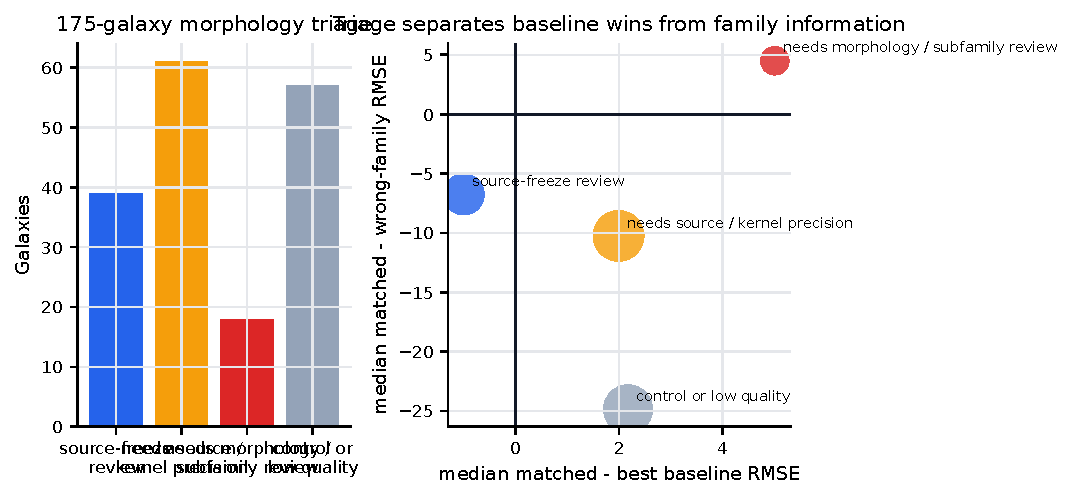
\includegraphics[width=0.92\linewidth]{figures/fig19_all_galaxy_triage.pdf}
\caption{All-SPARC morphology precision triage.  Left: the 175 galaxies are
partitioned into source-freeze candidates, source/kernel precision cases,
morphology/subfamily review cases, and control/low-quality cases.  Right:
median score differences show why the classes should not be collapsed into a
single win/loss statistic.  Some classes carry strong wrong-family information
without yet beating the best baseline.}
\end{figure}

\subsection{How morphology labels were assigned}

The morphology labels used in the present paper have different evidence grades.
This is why the manuscript distinguishes population preflights, all-galaxy
triage, and inspected single-galaxy endpoints.  The broad population layers use
available residual-blind metadata and proxy source fields; the four inspected
cases use object-specific source ledgers.  Table~\ref{tab:morphology-source-audit}
summarizes the assignment logic.

\begin{table}[H]
\centering
\caption{Morphology/readout source audit.  ``Proxy'' means sufficient for
preflight or triage but not for endpoint validation.}
\label{tab:morphology-source-audit}
\scriptsize
\resizebox{\linewidth}{!}{%
\begin{tabular}{p{0.17\linewidth}p{0.18\linewidth}p{0.31\linewidth}p{0.24\linewidth}}
\toprule
Layer or galaxy & Readout label status & Source basis & Claim boundary\\
\midrule
44-galaxy holdout preflights & proxy family labels &
SPARC rotation/mass-model metadata, type, inclination, radial coverage,
surface-brightness and gas/bulge proxy fields; train-only amplitude policies &
Preparation-level screen only; useful for matched-vs-wrong and shuffled-label
tests, not endpoint validation\\
175-galaxy all-SPARC triage & compiled current readout family &
Accepted-manifest table plus missing-observable ledger: source status,
confidence, caveats, missing fields, fallback policy, and next source gate &
Worklist and prioritization layer; endpoint velocities are used only after the
compiled protocol exists\\
NGC4013 & mixed exponential-disk / warp-vertical overlay lane &
H I and vertical-structure literature context
\cite{ZschaechnerRand2015NGC4013HI,Comeron2011NGC4013Vertical}; later
fresh-source review supports the lane, but the score remains retrospective &
Protocol-ready and replay-needed; not an accepted population endpoint\\
NGC5907 & projection-dominated mixed readout &
Warp, edge-on, and interaction/projection context
\cite{Sasaki1987NGC5907Warp,Shang1998NGC5907Warp,Wiegert2015EdgeOnISM} &
Accepted preliminary single-galaxy control; population validation still open\\
NGC7331 & exponential/vertical/outer-warp mixed lane &
H I warp/trajectory and vertical-scale context
\cite{Bosma1978NGC7331HI,Patra2018NGC7331ScaleHeight}; pure branch retained as
negative control &
Caveated accepted mixed case; broad outer window and pure-branch negative
remain explicit caveats\\
NGC4088 & warp/trajectory readout &
H I/interaction and warp/asymmetry source packet from the object-specific
ledger; B1 provenance and B2/B3 normalization remain caveated &
Strongest single inspected case; caveated endpoint, not a general law claim\\
\bottomrule
\end{tabular}
}
\end{table}

Thus the morphology determination is not uniform across all rows.  The broad
screens deliberately use weaker but residual-blind proxies to find where the
protocol is informative.  The inspected galaxies use stronger source packets,
but they still carry case-specific caveats.  This is why the paper does not
collapse the evidence into a single ``Tau wins'' or ``Tau fails'' statement.

\section{Numerical evidence}

\noindent\fbox{%
\begin{minipage}{0.94\linewidth}
\textbf{Claim levels used below.}
\begin{itemize}[leftmargin=*]
\item \textbf{Strong internal-preflight signal:} source-native readout formulas beat
wrong morphology families on the holdout split more often than shuffled labels
would predict.
\item \textbf{Moderate case evidence:} four inspected galaxies show local
matched-family improvement, but each remains caveated.
\item \textbf{Not shown:} population-level superiority over Newtonian,
MOND/RAR-like, or TPG/v6-like baselines.
\end{itemize}
\end{minipage}
}

\subsection{Population preflights}

The current executable analysis contains several preparation-level screens.  They
are useful because they separate morphology specificity from baseline
superiority.

\begin{table}[H]
\centering
\caption{Main population-level preflight outcomes.  These are internal
preflight results, not empirical validation.}
\small
\resizebox{\linewidth}{!}{%
\begin{tabular}{p{0.29\linewidth}cccc}
\toprule
Test & Holdout/sample & Beats wrong family & Beats TPG/v6 & Beats MOND-like\\
\midrule
Metadata readout proxy & 44 holdout & 0.568 & 0.636 & 0.614\\
Naive radial shell proxy & 44 holdout & 0.500 & 0.477 & 0.477\\
Source-native readout formulas & 44 holdout & 0.886 & 0.477 & 0.477\\
Readout-mixture proxy & 44 holdout & 0.455 & 0.500 & 0.455\\
L1 source-light screen & 66 screened & 53/66 & 17/66 all-baseline & --\\
\bottomrule
\end{tabular}
}
\end{table}

The strongest internal-preflight signal is the source-native readout-formula
preflight: the matched formula beats the wrong-formula mean in \(0.886\) of the
44 holdout galaxies, with a 1000-permutation shuffled-label null
\(p\simeq0.002\) for the mean matched-minus-wrong statistic and
\(p\simeq0.006\) for the beat-fraction statistic.  This records internal
label--formula compatibility in the frozen packet and motivates a specificity
hypothesis; it does not establish conditional or externally replicated
morphology specificity.
It does not support a stronger claim that the present readout formulas beat
TPG/v6, MOND-like, or RAR-like baselines as a population law.

Table~\ref{tab:robustness-0886} records robustness checks for the same
source-native formula result.  These checks are not independent discoveries;
they are stress tests of the headline matched-versus-wrong statistic.

\begin{table}[H]
\centering
\caption{Robustness checks for the \(0.886\) holdout matched-versus-wrong
fraction.  All rows use the frozen source-native formula labels and are
generated by \texttt{scripts/build\_source\_native\_readout\_robustness.py} or
\texttt{scripts/run\_source\_native\_carrier\_robustness.py}.}
\label{tab:robustness-0886}
\small
\resizebox{\linewidth}{!}{%
\begin{tabular}{lp{0.18\linewidth}p{0.18\linewidth}p{0.44\linewidth}}
\toprule
Test & Result & \(p\)-value & Detail\\
\midrule
Original holdout & 0.886 & -- &
44 holdout galaxies; mean matched-minus-wrong \(=-17.684\,{\rm km\,s^{-1}}\).\\
10k shuffled-label null & 0.886 & 0.0093 &
Seed 271828; beat-fraction statistic; null beats-wrong median \(=0.773\).\\
Bootstrap CI & 0.886 & -- &
Seed 271829; 10000 galaxy bootstrap interval \([0.795,0.977]\).\\
Error-weighted RMSE & 0.886 & -- &
Uses SPARC velocity-error weights; mean weighted matched-minus-wrong
\(=-17.758\,{\rm km\,s^{-1}}\).\\
Alternative split median & 0.841 & -- &
Seed 271830; 100 family-stratified splits; central 90\% range
\([0.773,0.909]\).\\
Family-balanced score & 0.832 & -- &
Mean of holdout per-family beat fractions; compact \(0.571\), exponential
\(0.857\), scale-tail \(1.000\), thick/flared \(0.900\).\\
Newtonian-carrier amplitude freeze & 0.955 & 0.0010 &
Train-only amplitudes fit around \(v_n^2\) rather than TPG/v6; mean
matched-minus-wrong \(=-51.131\,{\rm km\,s^{-1}}\), median
\(-53.425\,{\rm km\,s^{-1}}\); family-balanced beat fraction \(=0.929\);
beat-fraction null \(p=0.0010\).\\
\bottomrule
\end{tabular}
}
\end{table}

The Newtonian-carrier row is important because it asks whether morphology
specificity survives when the train-only amplitude residual is defined around
the baryonic Newtonian carrier \(v_n\) rather than the TPG/v6 carrier.  It does:
the matched-versus-wrong holdout fraction remains high, the median margin has
the same sign as the mean, and the family-balanced score remains high.  The
freeze-invariance audit in
\path{data/derived/source_native_carrier_robustness_freeze_invariance_audit.csv}
records that labels, kernels, source proxies, and train/holdout splits are
unchanged.  This strengthens the carrier-robustness of the internal
matched-versus-wrong statistic, but it still does not establish population-level superiority over
TPG/v6, MOND-like, RAR-like, or Newtonian baselines.

This outcome is not treated as a surprise to be hidden.  It is part of the
protocol.  If a galaxy is morphologically regular, approximately scalar in its
effective residual structure, or dominated by a smooth closure-like response,
then Newtonian, MOND/RAR-like, or TPG/v6-like curves can be strong.  In the
language of the present paper, those baselines may be good low-dimensional
readout limits.  The morphology-matched programme becomes distinctive only
where the source morphology selects a different readout subfamily and that
choice improves against wrong families and shuffled labels before any endpoint
repair.

\begin{figure}[H]
\centering
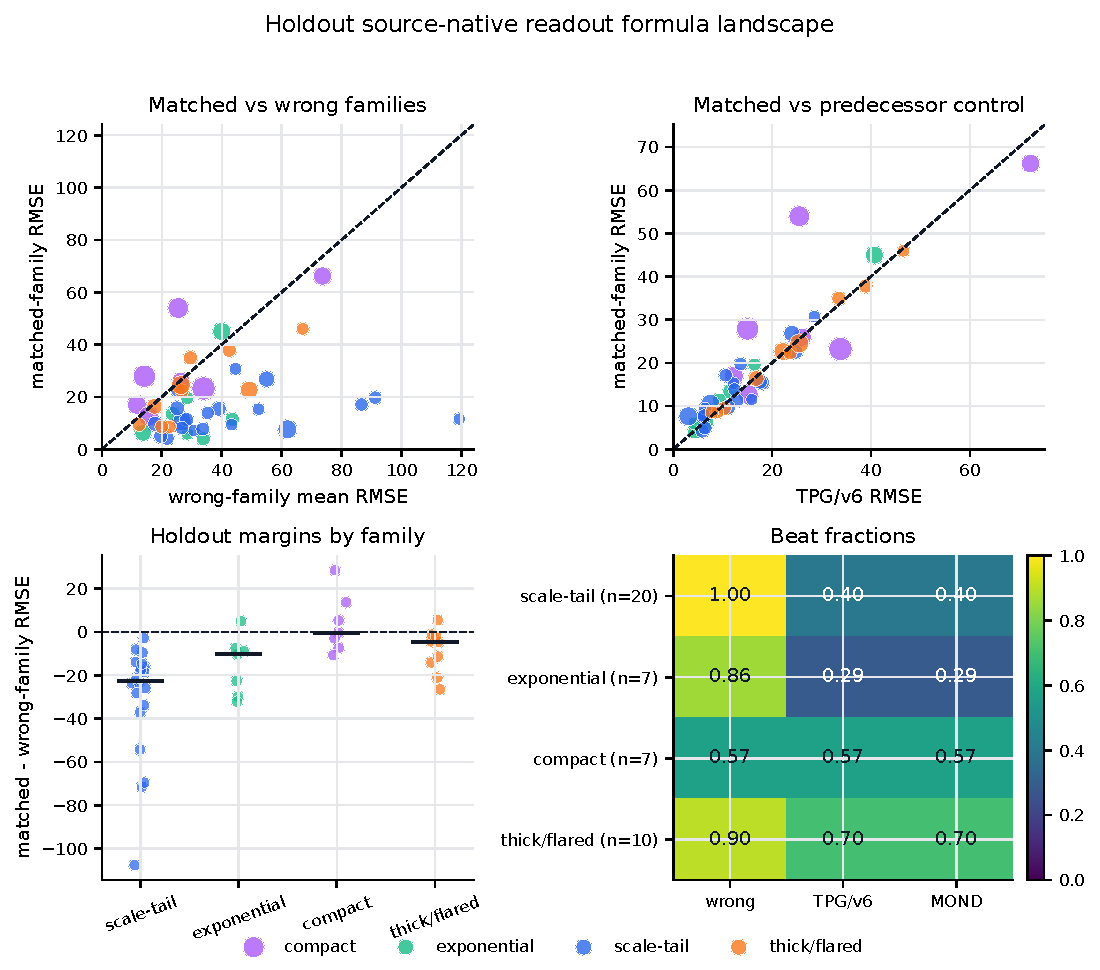
\includegraphics[width=0.86\linewidth]{figures/fig13_population_preflight_fractions.pdf}
\caption{Holdout source-native readout formula landscape.  The upper panels
compare matched-family RMSE against wrong-family and TPG/v6 controls for each
holdout galaxy.  Marker color denotes readout family and marker size tracks the
number of rotation-curve points.  The lower panels show family-level margins and
beat fractions.  The figure makes the main result visual: the matched families
often beat wrong morphology families, while baseline superiority remains mixed.}
\end{figure}

\begin{figure}[H]
\centering
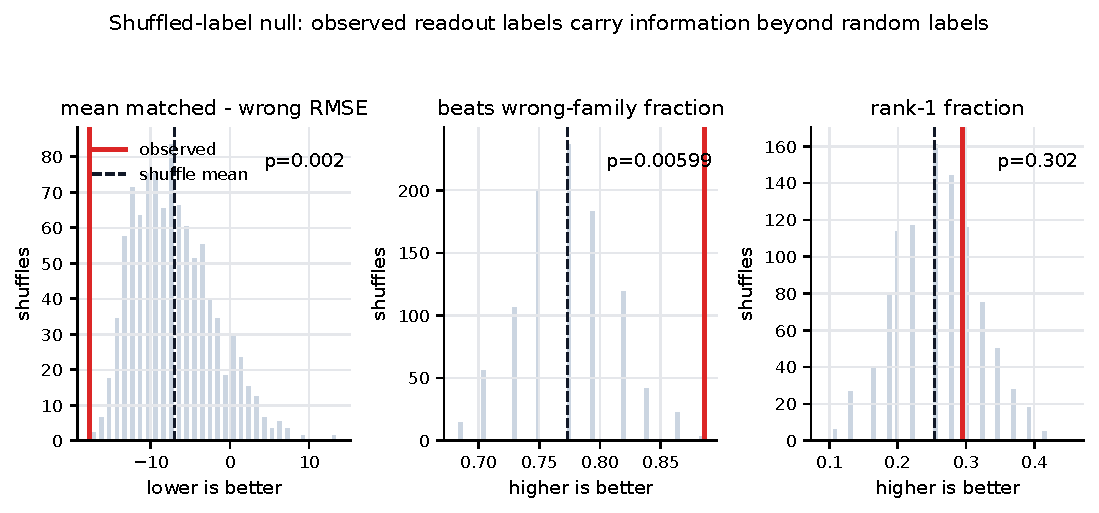
\includegraphics[width=0.86\linewidth]{figures/fig14_shuffled_null_control.pdf}
\caption{Shuffled-label null distributions for the source-native readout
formulas.  Grey histograms show 1000 morphology-label shuffles; red lines show
the observed holdout statistic.  The observed matched-minus-wrong mean and
beats-wrong fraction lie in the favorable tail of the shuffled null, while the
rank-1 statistic is weaker.}
\end{figure}

The negative readout-mixture proxy is also informative.  It shows that a mixture
layer cannot be supplied by coarse present-day proxy heuristics.  Mixture
weights need accepted source observables: projection, H I support, vertical
structure, interaction/history context, and a residual-blind normalization rule.

\begin{figure}[H]
\centering
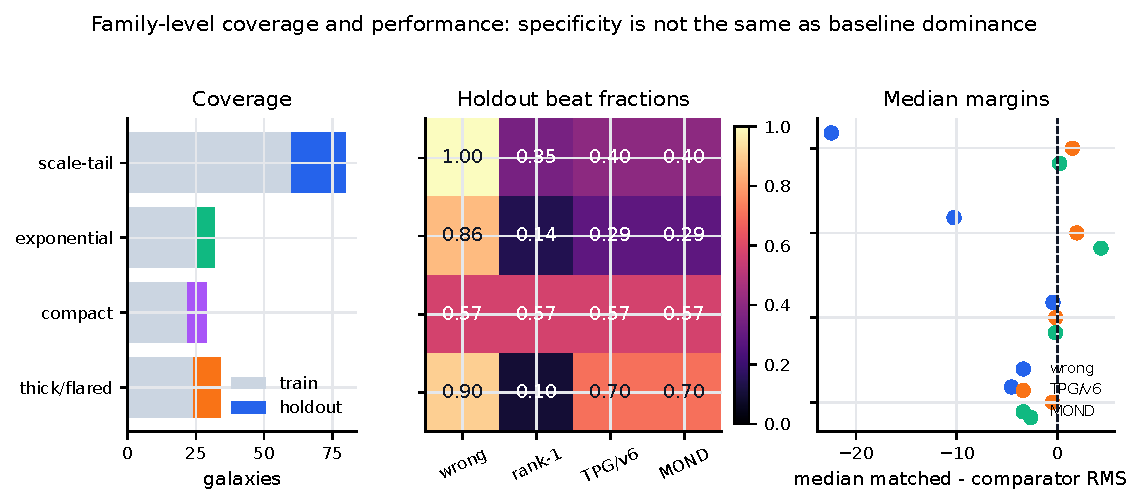
\includegraphics[width=0.86\linewidth]{figures/fig16_family_breakdown.pdf}
\caption{Family-level coverage and performance.  Left: train/holdout coverage
of the four one-dimensional source-native families.  Middle: holdout beat
fractions against wrong-family, rank-1, TPG/v6, and MOND-like comparators.
Right: median matched-minus-comparator RMSE margins.  The panel shows that
coverage, morphology specificity, and proxy baseline flags are distinct
quantities.  Baseline-comparator beat fractions are proxy-level flags, not
endpoint validation.}
\end{figure}

\subsection{Conditional-information and external matched-tracer audits}

Two later audits test whether the internal SPARC preflight can be promoted.
First, a repeated stratified cross-fitted audit on the frozen 45-galaxy A/C
packet supplies endpoint-residual-free observability and baryonic covariates,
then asks whether the projection contrast
\[
 X_{\rm proj}-\tfrac12(X_{\rm MOND}+X_{\rm RAR})
\]
adds held-out predictive information.  At the primary regularization the
baseline AUC is \(0.87395\), while the contrast changes AUC by \(-0.01891\),
log-loss improvement by \(-0.03994\), and Brier improvement by \(-0.01189\).
Both proper scores worsen for both declared baselines and all three frozen
regularizations.  This is a negative conditional predictive-increment audit,
not a proof that mathematical conditional mutual information is exactly zero.

Second, the public EDGE--CALIFA matched-resolution packet provides an external
operational homolog using CO(1--0), H\(\alpha\), stellar, dispersion, line-ratio,
and star-formation maps \cite{Levy2018EDGECALIFAKinematics,Wong2023EDGEData}.
The 17 galaxies in the published CO--H\(\alpha\) rotation analysis were excluded
before cohort selection.  A first source-only protocol admitted no object and
was preserved as a source-coverage failure.  A separately versioned,
source-developed protocol admitted eight galaxies before either terminal
velocity field was opened: NGC2639 for development and seven untouched objects
for confirmation.  One score-blind development support failure changed only
the requirement from all six to at least five of six occupied azimuthal sectors;
the source matrices, galaxies, five radial zones, rank-four covariance gate,
controls, velocity conversions, and decision thresholds remained fixed.

The velocity convention is material.  EDGE CO velocities use the radio
convention in the LSRK frame, whereas the CALIFA H\(\alpha\) velocities use the
optical convention.  The frozen endpoint first applies the public
LSRK-to-heliocentric correction and converts both tracers separately to the
relativistic convention, following Appendix A of
Levy et al. \cite{Levy2018EDGECALIFAKinematics}; only then is the contrast
formed.  A per-zone intercept absorbs an arbitrary constant zero point.

For a declared source span \(S\), the endpoint uses
\[
 Q(S)=y^{\mathsf T}P_{\perp}(S)^{\mathsf T}
 \left[P_{\perp}(S)\Sigma P_{\perp}(S)^{\mathsf T}\right]^{+}
 P_{\perp}(S)y,
\]
and the per-galaxy matched-versus-wrong contrast
\[
 D_g=\tfrac13\left(Q_{\rm radial}+Q_{\rm phase}+Q_{\rm cross}\right)
      -Q_{\rm correct}.
\]
This construction has an exact identifiability boundary.  Because each source
matrix has full column rank, every invertible basis change \(R\) obeys
\[
 P_{\perp}(SR)=P_{\perp}(S),
 \qquad Q(SR)=Q(S).
\]
The score can therefore test a source subspace, but cannot select an oriented
coefficient vector or the sign of a terminal prediction inside it.  In
particular \(S\) and \(-S\) are score-equivalent while an otherwise unspecified
fixed coordinate vector would give opposite candidate terminal vectors.  A
physical prediction must instead supply the signed load and ordered forward
descent before endpoint access, schematically
\[
 H_B\delta M=j_s,
 \qquad
 z_A=J_{A\leftarrow M}\delta M+J_{A\leftarrow OS}\xi_{OS},
 \qquad
 c_{OS}=Q_{OS}(z_A),
 \qquad
 h_{\tau}=R_T(c_{OS})-R_T(Q_{OS}(0)),
 \qquad
 h_{\perp}=P_{\perp{\rm std}}h_{\tau}.
\]
Here the stabilized body response is solved and frozen before the post-body
observer--source channel.  The irreducible observer--source load \(\xi_{OS}\)
and source-derived stable resolution map \(Q_{OS}\) are not part of a
simultaneous body solve.  On a stable linearized branch these maps may be
compressed into the usual Jacobian notation, but the body-driven product
\(J_TJ_OH_B^{-1}j_s\) is only the \(\xi_{OS}=0\) restriction.  A Tau-specific
first-order direction also requires \(h_{\perp}\ne0\) relative to a complete
frozen standard comparator.  The existing conditional CHDF/ordered-disk
completion does not supply this packet: the same pure source shells admit a
direct-product control with zero disk--CHDF mixed derivative, so physical
occupation and the signed terminal law remain open.
All correct and wrong-family constructions have source rank 16 and leave a
rank-four projected terminal covariance.  The primary population test is the
exact one-sided shared-sign permutation of \(\overline D\) over all \(2^7\)
sign vectors; radial-reversal, phase-rotation, and cyclic cross-galaxy controls
use the corresponding studentized max-\(T\) distribution.

\begin{table}[H]
\centering
\caption{Frozen EDGE--CALIFA seven-galaxy confirmatory endpoint.  A positive
\(D_g\) favors the matched morphology over the mean equal-rank wrong-family
control.}
\small
\begin{tabular}{lr}
\toprule
Quantity & Result\\
\midrule
Mean \(D_g\) & \(-0.058679\)\\
Median \(D_g\) & \(+0.110202\)\\
Positive galaxies & \(4/7\)\\
Exact one-sided primary \(p\) & \(0.6015625\)\\
Radial/phase/cross max-\(T\) adjusted \(p\) & \(0.9766/0.9453/0.3359\)\\
Frozen decision & prevalidation fail\\
\bottomrule
\end{tabular}
\label{tab:edge-califa-confirmatory}
\end{table}

The mean, positive-fraction, primary-significance, and all three control gates
fail; only the positive median condition holds.  No post-opening replacement,
mask change, alternate sector rule, or new score is permitted in this packet.
An independent implementation rebuilds all \(7\times20\) terminal coefficients
from the checksum-matched public HDF5 file, with maximum absolute coefficient
difference \(3.55\times10^{-15}\,{\rm km\,s^{-1}}\), and reproduces all 32
declared hash, rank, projection, score, and inference checks.  It also records
that the local hash chain does not independently prove freeze chronology, the
original endpoint JSON does not bind the coefficient CSV, and the public raw
packet is referenced rather than vendored.
The result rejects this development-informed morphology-alignment proxy as an
external promotion route.  It neither falsifies the broader Tau Core
architecture nor identifies standard astrophysics as complete: the declared
standard span is not exhaustive and no unique Tau coefficient law was supplied.
Conversely, that limitation would also have prevented a positive result from
being called Tau-specific.  A claim-raising successor must use an independent
survey or release, a source-derived signed \(h_{\tau}\), a complete declared
standard comparator, and a new freeze before endpoint access.

\subsection{External rotation-search ladder beyond the EDGE endpoint}

Several already-frozen public-data routes constrain what a successor may
claim.  They are kept separate because they test different objects and do not
form one combined significance.  The LITTLE THINGS lane uses published dwarf
mass models \cite{Oh2015LITTLETHINGS}.  The PHANGS lanes combine public
CO kinematics, MUSE ionized-gas products, and residual-blind stellar-structure
maps \cite{Lang2020PHANGSKinematics,Emsellem2022PHANGSMUSE,
Querejeta2021PHANGSStructures}.

\begin{table}[H]
\centering
\caption{Current external rotation-search ladder.  A numerical feature is not
promoted when its source-integrity, specificity, identifiability, or
predeclared support gate fails.}
\small
\begin{tabularx}{\linewidth}{p{0.18\linewidth}p{0.27\linewidth}X}
\toprule
Route & Frozen numerical result & Claim-safe decision\\
\midrule
LITTLE THINGS & \(N=14\), 313 points; matched-minus-TPG mean RMSE
\(-0.101\,{\rm km\,s^{-1}}\), matched-minus-MOND
\(+0.649\,{\rm km\,s^{-1}}\) & Mixed prospective transfer of one frozen
scale-tail family; below the \(N\ge15\) replication gate and not a
multi-family attribution test.\\
PHANGS low-order orthogonal & Three eligible galaxies;
\(\chi^2=23.17/30\), \(p=0.8082\) & The declared morphology-orthogonal
low-order component is consistent with zero; the earlier wrong-family hint
does not replicate.\\
PHANGS two-body population & Frozen \(m=2\):
\(\chi^2=77.606/20\), \(p=9.97\times10^{-9}\); \(m=1\) control also non-null,
\(p=8.26\times10^{-11}\) & Numerical structure is preserved, but the
source-label audit contradicts bar absence for NGC4321 and leaves IC5332
unvalidated; no morphology-conditioned promotion.\\
PHANGS radial body projection & Four confirmatory galaxies & The mandatory
12-sector occupancy gate fails in the outer common-support zones; no
individual or aggregate \(Q\) is released, and the 19-galaxy product family is
exhausted for replacement.\\
NGC4254 source coordinate & Direct beam-safe \(m=2\) candidate has source
range \([0.0466,0.1017]\), measurement 95\% interval \([0.0612,0.1229]\), and
sign probability 0.996; the \(m=1\) control fails & Internally robust
source-side candidate only.  A free terminal gain exactly saturates a scalar
endpoint, and identical source states admit primitive witness gains
0.3333--0.6667; endpoint scoring remains closed.\\
\bottomrule
\end{tabularx}
\label{tab:external-rotation-ladder}
\end{table}

The PHANGS radial source matrices have an additional source-only property: a
unique Euclidean rank-four approximation captures 0.865--0.939 of their
normalized Frobenius energy in the five development galaxies.  This is a
useful compression diagnostic, not evidence for physical four-dimensional
descent, because the source-coordinate metric, CHDF roles, body connection,
terminal map, and occupation law are not derived by the singular-value
decomposition.

Taken together, these routes locate two real but non-promotable candidates:
the PHANGS low-order differential field and the NGC4254 source coordinate.
Neither supplies a signed, unit-calibrated terminal vector outside a complete
standard tangent space.  The next valid endpoint must therefore begin from
the forward packet above rather than from another freely oriented source span
or a post-open repair of these samples.

\subsection{Finite morphology representation versus the parent body}

The negative ladder tests finite morphology representations, not direct access
to a source-complete parent body.  Let
\(\Phi_k:\mathcal M_\tau\rightarrow\mathcal Z_k\) be the representation frozen
for endpoint \(k\), and let \(T_k\) denote the complete
body--channel--observer-resolution--terminal composition.  A descended law
\(T_k=f_k\circ\Phi_k\) exists only if
\begin{equation}
\Phi_k(M_1)=\Phi_k(M_2)\quad\Longrightarrow\quad
T_k(M_1)=T_k(M_2).
\label{eq:fibre-sufficiency}
\end{equation}
If the terminal differs within one \(\Phi_k\) fibre, the representation is
non-identifying even if a richer body exists.  In the linear source case,
\begin{equation}
P_\perp(S)=I-S(S^{\mathsf T}WS)^{-1}S^{\mathsf T}W,\qquad
u\in\ker(S^{\mathsf T}W)\quad\Longrightarrow\quad P_\perp(S)u=u.
\label{eq:omitted-direction}
\end{equation}
Thus an omitted physical component cannot be recovered by coefficients inside
the declared source span.  The seven EDGE source matrices are \(20\times16\),
so each leaves four linear directions outside that representation.  This does
not show that Nature occupies an omitted direction; it shows why failure of a
finite proxy is not logically identical to falsification of every possible
\(M_\tau\).

The corresponding anti-rescue result is equally exact.  Once terminal vector
\(y\) has been inspected, augmenting the source matrix to \(S'=[S,y]\), with
the weighted Moore--Penrose projector used if \(S'\) is rank deficient, gives
\begin{equation}
P_\perp(S')y=0.
\label{eq:post-open-saturation}
\end{equation}
An endpoint-informed morphology refinement can therefore fit the same packet
by construction and has no confirmatory force.  The only admissible iteration
is to construct a richer \(\Phi_{k+1}\), its \(Q_{OS}\), sign, units, and
terminal descent from source-only information, freeze them, and evaluate a new
untouched survey or release.

\subsection{Inspected single-galaxy cases}

The reproducibility code also contains four inspected cases.  They are heterogeneous and
should not be combined into a population validation claim.

\begin{table}[H]
\centering
\caption{Four inspected readout cases.  RMSE values are in
\({\rm km\,s^{-1}}\).}
\small
\resizebox{\linewidth}{!}{%
\begin{tabular}{lcccp{0.21\linewidth}p{0.24\linewidth}}
\toprule
Galaxy & Matched & Best baseline & Best wrong & Status & Interpretation\\
\midrule
NGC4013 & 10.61 & 10.88 & 11.37 &
retroactive/caveated & protocol-ready, replay needed\\
NGC5907 & 16.37 & 16.79 & 16.85 &
accepted preliminary & mixed projection readout\\
NGC7331 & 22.26 & 23.47 & 22.67 &
caveated accepted & mixed branch positive; pure branch negative\\
NGC4088 & 11.62 & 25.40 & 37.87 &
caveated accepted & strongest single case; law-level caveats\\
\bottomrule
\end{tabular}
}
\end{table}

Across these four inspected rows, the source- or morphology-matched readout
beats the best local baseline and the inspected wrong-family controls in all
four cases.  This is a retrospective case-level compatibility pattern.  It is not
population validation, and these cases were not selected as a statistically
independent validation sample: NGC4013 remains retrospective, NGC7331 carries a
broad outer-window caveat, and NGC4088 still has source-provenance and
law-level normalization caveats.
The object-level morphology context is residual-blind and source-ledger based:
NGC4013 is supported by H I and vertical-structure studies
\cite{ZschaechnerRand2015NGC4013HI,Comeron2011NGC4013Vertical};
NGC5907 by warp, edge-on, and interaction/projection context
\cite{Sasaki1987NGC5907Warp,Shang1998NGC5907Warp,Wiegert2015EdgeOnISM};
NGC7331 by H I warp/trajectory and vertical-scale context
\cite{Bosma1978NGC7331HI,Patra2018NGC7331ScaleHeight}.  These references
motivate the readout lanes and caveats; they are not by themselves endpoint
evidence.

\begin{figure}[H]
\centering
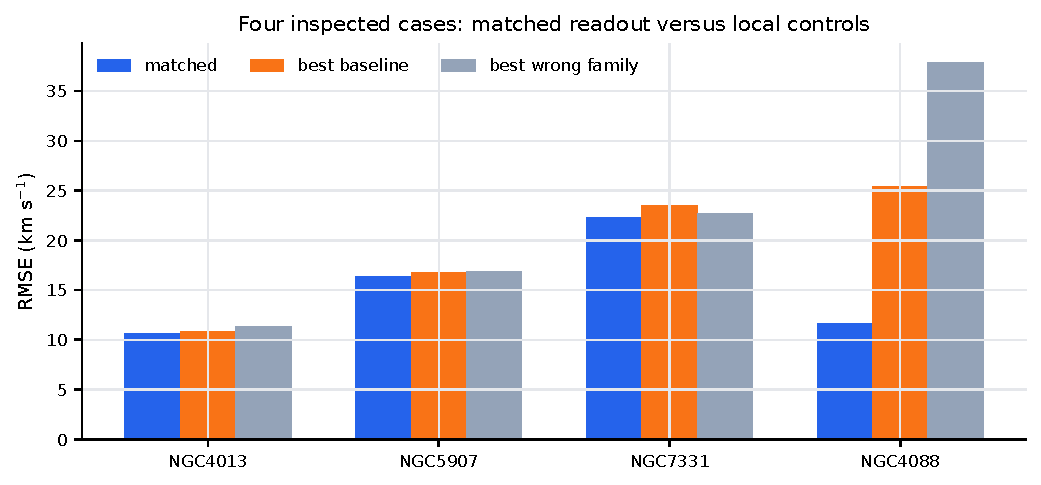
\includegraphics[width=0.86\linewidth]{figures/fig15_four_case_rmse_comparison.pdf}
\caption{Four inspected cases.  The matched readout is better than the best
local baseline and best inspected wrong-family control in all four rows.  The
claim remains case-level and caveated because the evidence packets are
heterogeneous.}
\end{figure}

\begin{figure}[H]
\centering
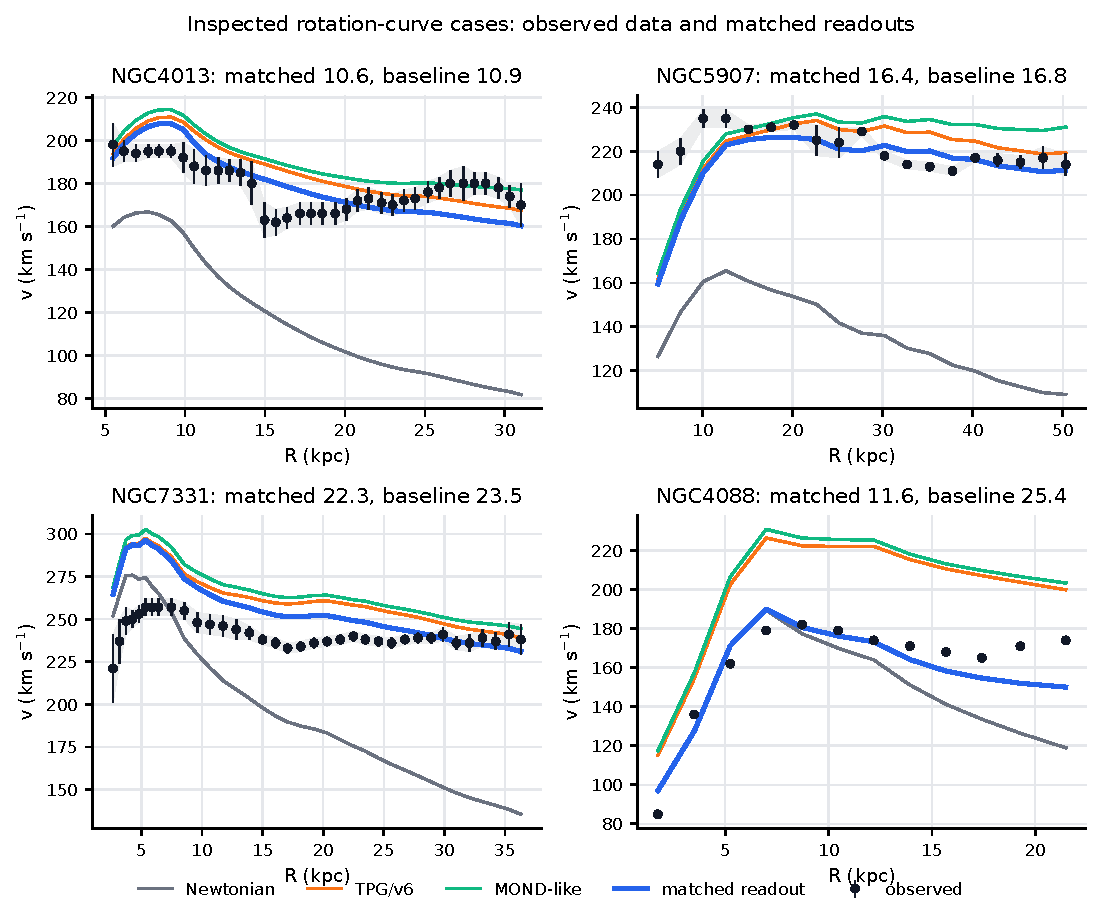
\includegraphics[width=0.98\linewidth]{figures/fig17_inspected_rotation_curves.pdf}
\caption{Rotation-curve view for the four inspected endpoint cases.  Points are
observed SPARC rotation speeds with reported error bands.  The matched readout
curve is compared with the
Newtonian baryonic curve, the fixed TPG/v6 predecessor comparator, and the
MOND-like comparator available in the reproducibility package.  Panel titles
report matched and best-baseline RMSE values.}
\end{figure}

\begin{figure}[H]
\centering
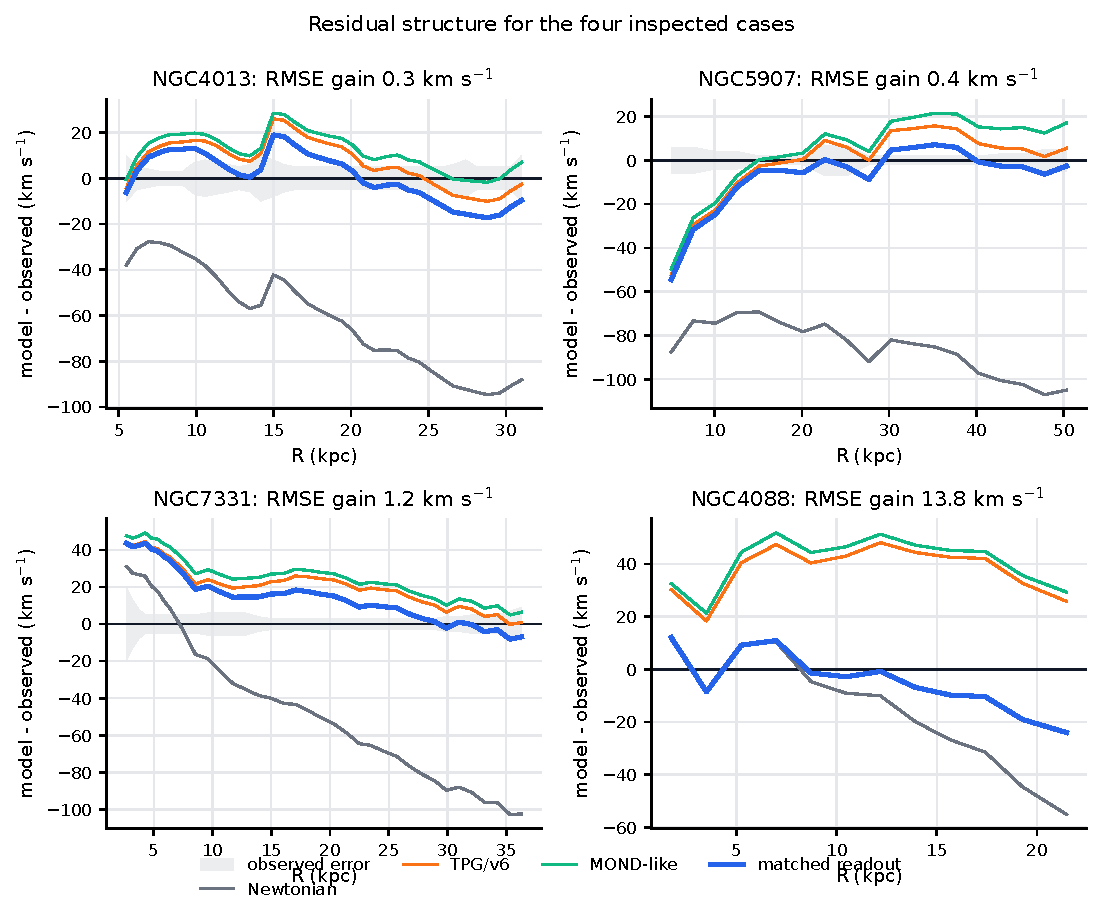
\includegraphics[width=0.98\linewidth]{figures/fig18_inspected_rotation_residuals.pdf}
\caption{Signed residuals for the same four inspected cases,
\(\Delta v=v_{\rm model}-v_{\rm obs}\), with the observational error band shown
around zero where available.  Residual panels are important because
an endpoint can look visually reasonable while leaving systematic radial
structure.  Panel titles report the matched improvement over the best local
baseline in \({\rm km\,s^{-1}}\).}
\end{figure}

These rotation and residual panels are the most direct visual summary of the
present single-galaxy evidence.  NGC4088 shows the clearest endpoint-style gain:
the matched warp/trajectory readout reduces a large baseline mismatch over much of
the measured radial range.  NGC5907 and NGC7331 are more modest: the matched
mixed readout improves the score, but the curves remain close enough to strong
smooth controls that the result should be read as a source-frozen
case-improvement, not as a new law.  NGC4013 is scientifically useful for a
different reason: it shows how a mixed vertical/warp readout can become
competitive, while also illustrating why retrospective cases need replay before
promotion.

The TPG/v6 curves in these panels are therefore not a disposable comparison.
They are a serious predecessor-control: when they are already close to the
observations, a new morphology-matched readout must explain why it adds
source-specific information rather than merely reproducing a smooth closure
shape.  This is why the paper separates three claims: morphology specificity
against wrong families, competition against TPG/v6 or MOND-like controls, and
full endpoint-grade validation.

\begin{figure}[H]
\centering
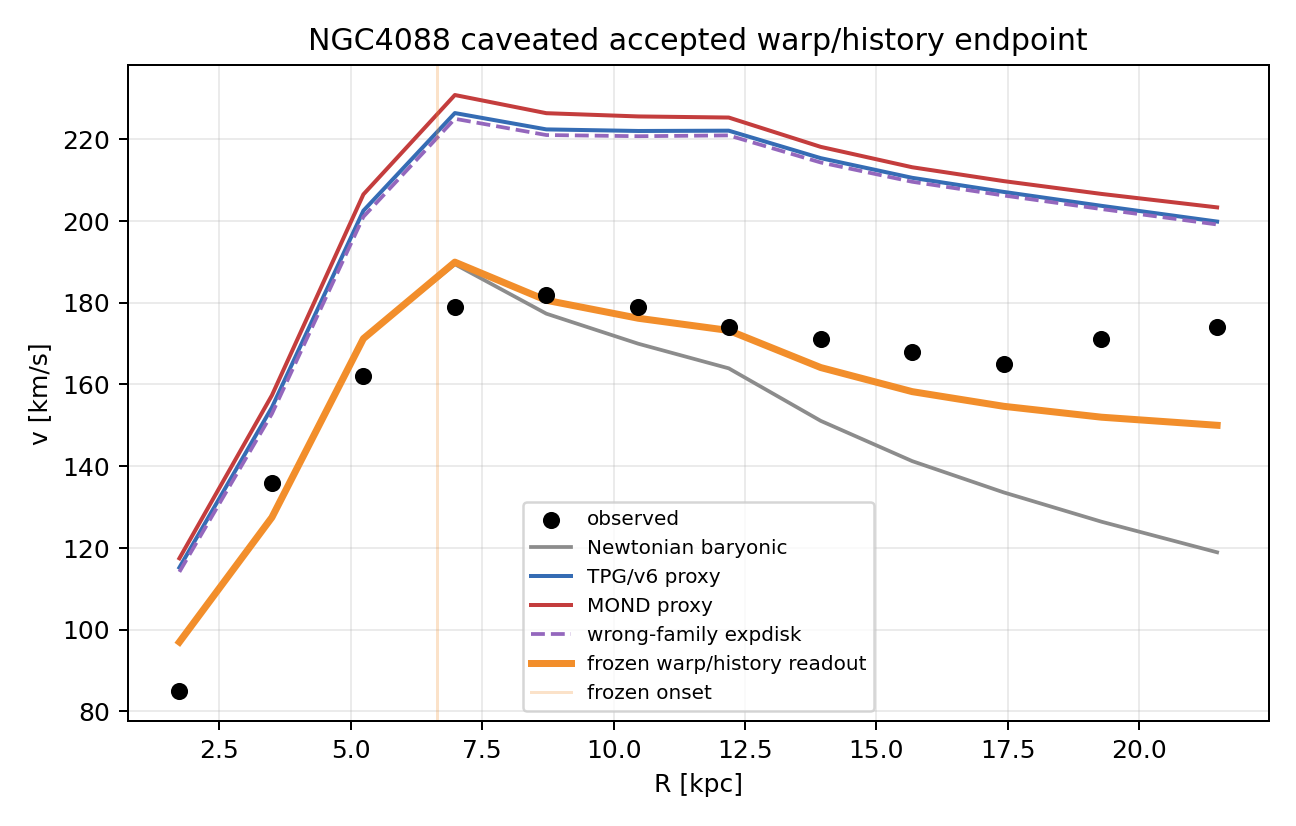
\includegraphics[width=0.78\linewidth]{figures/fig10_ngc4088_warp_history_accepted_endpoint.png}
\caption{NGC4088 caveated warp/trajectory endpoint.  This is the strongest
single-galaxy result in the current code, but remains a preliminary control endpoint,
not population validation.}
\end{figure}

An object-specific freeze note,
\path{reports/ngc4088_object_specific_freeze_note.md}, records the
residual-blind source fields, current blockers, and claim boundary for this
case.  The note is included because NGC4088 is visually compelling but should
not be allowed to carry a population-level claim by itself.

\subsection{Unchanged-law transfer to UGC08490/NGC5204}

The strongest direct test of whether the NGC4088 result generalizes is to keep
its formula class unchanged and replace only the source-owned galaxy inputs.
For UGC08490/NGC5204, a three-dimensional TiRiFiC tilted-ring analysis supplies
a source-native two-plane H I warp: the first nonzero tip occurs at
\(156\) arcsec and the inner and outer planes differ by
\(41.1\pm5.7\) degrees \cite{Jozsa2007WarpedDisks}.  Converting the angular
onset on the SPARC distance scale and dividing by the published H I radius
gives the frozen value
\[
x_w=0.4508763.
\]
Before opening the pointwise SPARC curve, the transfer retained
\(q_{\rm warp}=1\), \(\sigma_{\rm warp}=+1\), \(p=1\), and
\(\lambda_w=x_wV_{\rm flat}^2\), producing
\(\lambda_w=2785.50\,{\rm km^2\,s^{-2}}\).  The manifest was then hashed and
the endpoint was scored by a separate script.  Since UGC08490 had been opened
in earlier, different tracer analyses, this is a retrospective frozen transfer,
not a prospective blind endpoint.  Moreover, the published SPARC \(R_{\rm HI}\)
and \(V_{\rm flat}\) are observed summary inputs, so the test is not a
zero-information dimensional-amplitude prediction.

\begin{table}[H]
\centering
\caption{UGC08490 unchanged NGC4088-class transfer.  No target parameter is
fitted to the pointwise endpoint, except in the explicitly fit-aided halo
comparators.  RMSE values are in \({\rm km\,s^{-1}}\).}
\small
\begin{tabular}{lcc}
\toprule
Model or control & RMSE & Role\\
\midrule
NFW halo + baryons & 1.20 & two-parameter endpoint fit\\
Pseudo-isothermal halo + baryons & 1.55 & two-parameter endpoint fit\\
Fixed MOND & 8.78 & fixed standard comparator\\
Fixed TPG/v6 & 12.75 & fixed predecessor comparator\\
Frozen source-correct warp transfer & 29.70 & matched transfer\\
Wrong NGC4088 onset & 31.64 & morphology control\\
Wrong quadratic turn-on & 31.90 & morphology control\\
Newtonian baryons & 44.87 & fixed carrier limit\\
\bottomrule
\end{tabular}
\end{table}

The correct source onset therefore performs better than the wrong onset and
wrong turn-on controls, while reducing the Newtonian RMSE by
\(15.17\,{\rm km\,s^{-1}}\).  That ordering is suggestive but not decisive: a
circular block bootstrap gives only \(0.9436\) probability of a lower mean
squared error than the wrong-onset control, with a 95\% interval that crosses
zero.  The endpoint-informed best-onset diagnostic is \(x_w=0.4937\), close to
the source value, but improves RMSE by only \(0.074\,{\rm km\,s^{-1}}\); it is
recorded and not used to repair the frozen law.

The standard-comparator failure is unambiguous.  Ten of the thirty points lie
inside the warp onset, where the transferred law is exactly Newtonian although
the large rotation discrepancy is already present.  Even outside the onset,
the frozen transfer has \(26.10\,{\rm km\,s^{-1}}\) RMSE, compared with
\(7.13\,{\rm km\,s^{-1}}\) for fixed MOND.  Thus the outer warp is a real and
informative morphology component, but it is not the complete carrier of this
galaxy's rotation discrepancy.  The result rejects the current one-component
NGC4088 warp law as a universal complete rotation law.  It does not reject a
multi-component source-frozen readout, because the source description itself
also contains an inner irregular/ringed disk that the transferred kernel does
not represent.  No same-endpoint enrichment is permitted.

\begin{figure}[H]
\centering
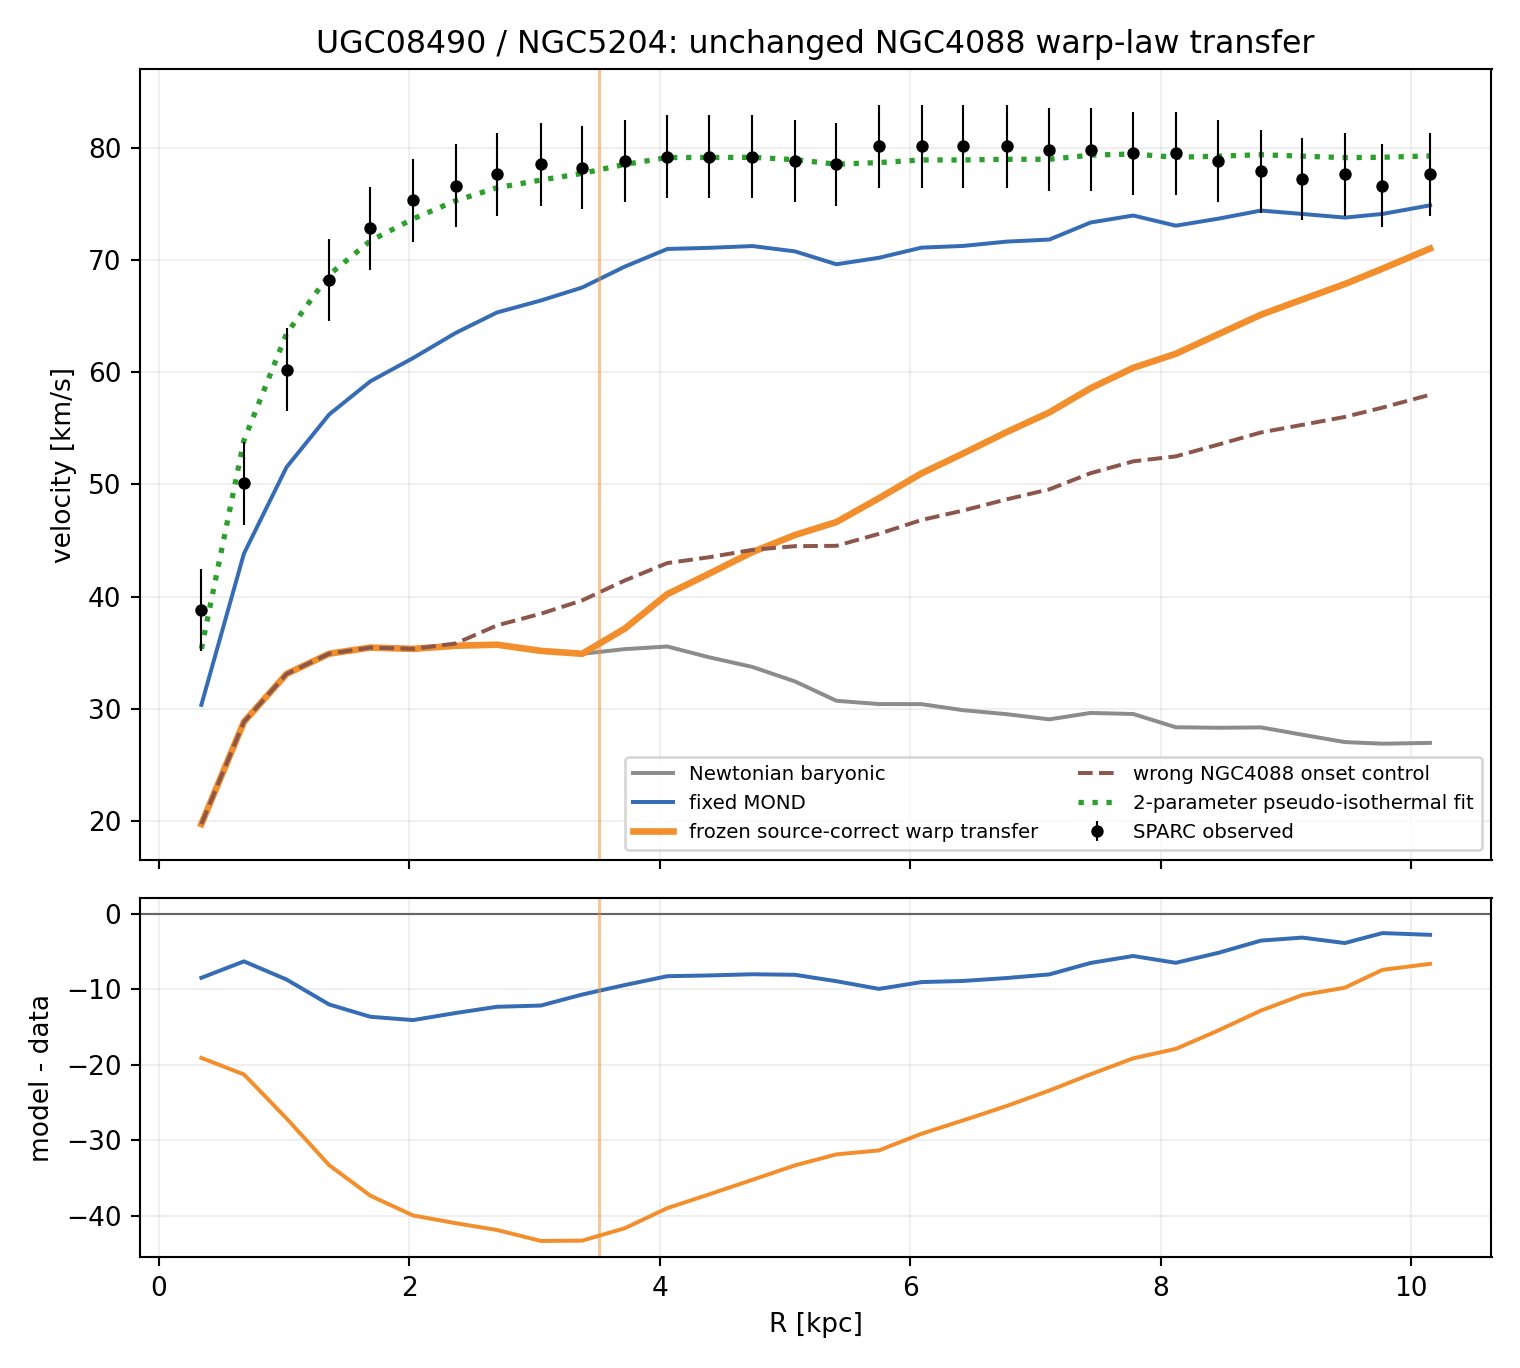
\includegraphics[width=0.86\linewidth]{figures/fig_ugc08490_ngc5204_ngc4088_class_transfer_v01.png}
\caption{Retrospective unchanged-law transfer to UGC08490/NGC5204.  The
source-correct warp onset beats the wrong-onset morphology control but remains
far below the observed curve and is decisively worse than fixed MOND and
fit-aided halo comparators.  The lower panel shows signed residuals.}
\end{figure}

\subsection{Second unchanged-law replication: UGC03580/UGC3580}

The same Jozsa tilted-ring study supplies an independent member of the
source-selected warp class.  For UGC03580/UGC3580 the inner reference plane is
\(i=67.2\) degrees, \({\rm PA}=96.3\) degrees; the first nonzero source tip is
\(5.5\pm3.9\) degrees at \(180\) arcsec, and the mean inner/outer mutual
inclination is \(13.9\pm2.5\) degrees \cite{Jozsa2007WarpedDisks}.  The source
explicitly calls this warp less significant than those of NGC2541 and NGC5204
and treats a direct rotation-rise/warp connection cautiously.  Those caveats
are retained rather than converted into a stronger morphology label.

On the SPARC distance and H~I-radius scale the frozen onset is
\[
x_w=0.9045639,
\qquad
\lambda_w=x_wV_{\rm flat}^2
=14406.48\,{\rm km^2\,s^{-2}}.
\]
The class-law sign, binary activation and linear turn-on were copied unchanged,
and the freeze script did not open the local pointwise curve.  UGC03580 had,
however, appeared in earlier repository endpoint analyses, so this remains a
retrospective replication.  A source-native angular-denominator sensitivity
\(x_w=180/240=0.75\) and the published outer-speed normalization were also
declared before this scoring script.

\begin{table}[H]
\centering
\caption{UGC03580 unchanged NGC4088-class replication.  Full-curve RMSE values
are in \({\rm km\,s^{-1}}\).  The two halo rows are explicitly fit-aided.}
\small
\begin{tabular}{lcc}
\toprule
Model or control & RMSE & Role\\
\midrule
Pseudo-isothermal halo + baryons & 14.99 & two-parameter endpoint fit\\
NFW halo + baryons & 17.39 & two-parameter endpoint fit\\
Wrong UGC08490 onset & 24.56 & morphology control\\
Wrong NGC4088 onset & 25.29 & morphology control\\
Fixed TPG/v6 & 25.49 & fixed predecessor comparator\\
Fixed MOND & 27.17 & fixed standard comparator\\
Source-H~I denominator sensitivity & 27.68 & predeclared sensitivity\\
Newtonian baryons & 36.01 & fixed carrier limit\\
Frozen source-correct transfer & 38.04 & matched transfer\\
\bottomrule
\end{tabular}
\end{table}

The source-correct onset does not preserve the morphology ordering seen in
UGC08490.  Its full-curve RMSE is worse than Newtonian baryons, fixed MOND, and
both earlier-onset morphology controls.  Against the UGC08490-onset control,
the circular block-bootstrap interval for the primary-minus-control mean
squared error is strictly positive (\(58.3\) to \(2088.2\)
\({\rm km^2\,s^{-2}}\)); only \(0.00015\) of draws favour the primary.
Inside \(R_{\rm HI}\), the matched transfer modestly improves Newtonian RMSE
from \(31.66\) to \(29.68\,{\rm km\,s^{-1}}\), but remains worse than fixed
MOND at \(28.07\,{\rm km\,s^{-1}}\).

Three SPARC points lie beyond \(R_{\rm HI}\).  There the unchanged kernel
\[
C_{\rm warp}(x)=\max\!\left(0,\frac{x-x_w}{1-x_w}\right)
\]
continues above unity, reaching \(4.72\), and strongly overshoots.  This is a
structural failure of the uncapped class law, not a licence to cap it after
seeing the endpoint.  A bounded or plateauing two-plane kernel is a new law
that must be derived from source geometry and tested on another target.  Thus
the current replication rejects the uncapped one-component NGC4088 law as a
universal warp-class rotation law while leaving the broader morphology/readout
programme open.

\begin{figure}[H]
\centering
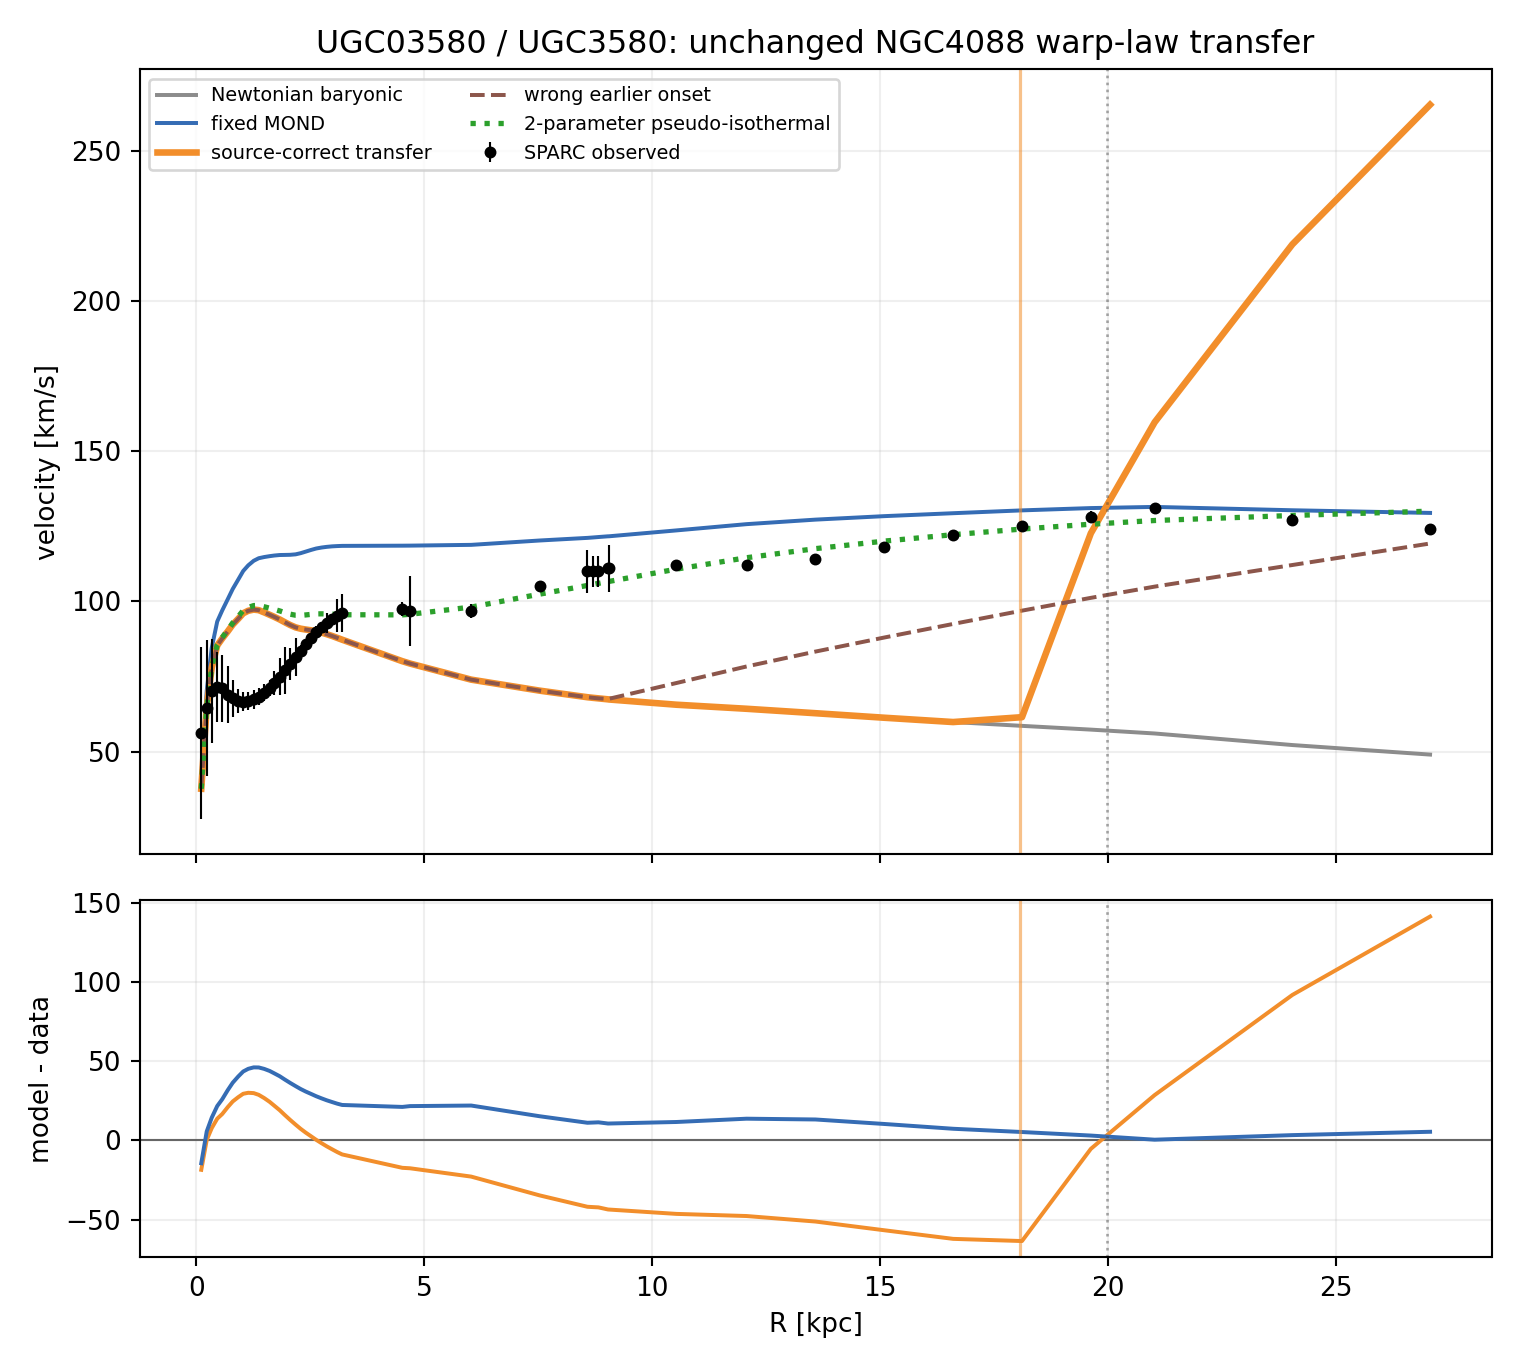
\includegraphics[width=0.86\linewidth]{figures/fig_ugc03580_ugc3580_ngc4088_class_transfer_v01.png}
\caption{Retrospective UGC03580/UGC3580 replication.  The source-correct onset
activates only in the outermost region and the uncapped continuation overshoots
beyond \(R_{\rm HI}\).  Earlier wrong-onset controls fit the full curve better,
so the UGC08490 morphology-ordering signal does not replicate.}
\end{figure}

\subsection{Source-only radial two-plane morphology refinement}

The failed transfer identifies two distinct objects that the scalar proxy had
conflated: the source morphology and the terminal law.  The endpoint cannot be
used to repair either one.  We therefore return only to the source table and
transcribe its radius, H~I surface density, inclination, position angle, spin
normal, tip and line-of-nodes fields.  The published rotation-velocity columns
and the SPARC endpoint are excluded from this construction.  Seventeen rings
lie inside the published terminal support at \(375\) arcsec; the \(420\)-arcsec
row is retained only as a declared support sensitivity.

At radius \(R\), the local disk plane is represented by the source orientation
normal
\[
\mathbf n(R)=
\bigl(
\sin i(R)\sin {\rm PA}(R),
-\sin i(R)\cos {\rm PA}(R),
\cos i(R)
\bigr)\in S^2.
\]
The inner reference plane is fixed by the published
\(i_0=67.2\) degrees and \({\rm PA}_0=96.3\) degrees.  As a source-only summary,
the outer plane \(\mathbf n_{\rm out}\) is \emph{defined}, rather than uniquely
derived, as the unweighted normalized chordal mean of the five ring normals on
the published \(240\)--\(375\)-arcsec outer range.  Adjacent source rings are
connected by shortest great-circle interpolation.  If
\(\theta_j=\arccos(\mathbf n_j\cdot\mathbf n_{j+1})\) and
\(\eta\in[0,1]\), the segment is
\[
\mathbf n_j(\eta)=
\frac{\sin[(1-\eta)\theta_j]}{\sin\theta_j}\mathbf n_j
+
\frac{\sin(\eta\theta_j)}{\sin\theta_j}\mathbf n_{j+1}.
\]
This gives a radial orientation field without Euclidean interpolation off the
unit sphere.  A bounded source morphology invariant is then
\[
\delta_{\rm tilt}(R)
=1-\mathbf n_0\cdot\mathbf n(R),
\qquad 0\leq\delta_{\rm tilt}\leq2,
\]
and the local connection magnitude between sampled rings is
\[
\kappa_j=
\frac{\theta_j}{R_{j+1}-R_j}.
\]
Neither quantity is identified here with a velocity correction.

The reconstructed inner/outer plane separation is \(14.297\) degrees, versus
the independent Table~4 value \(13.9\pm2.5\) degrees, a difference of only
\(0.159\) quoted standard deviations.  The maximum supported discrepancy
between the orientation-derived and tabulated normals is \(0.085\) degrees;
the maximum reconstructed-tip discrepancy is \(0.093\) degrees.  The inner
defect is exactly zero through the published flat inner region, and sampled
great-circle interpolation preserves unit norm to \(1.2\times10^{-16}\).
Source-only alternatives move the outer mean plane by \(1.487\) degrees for
H~I-density weighting, \(1.806\) degrees when the beyond-support ring is
included, \(2.217\) degrees under every-other-ring thinning, and at most
\(1.365\) degrees under leave-one-outer-ring-out deletion.  All four shifts
remain below the published \(2.5\)-degree Table~4 uncertainty.

\begin{figure}[H]
\centering
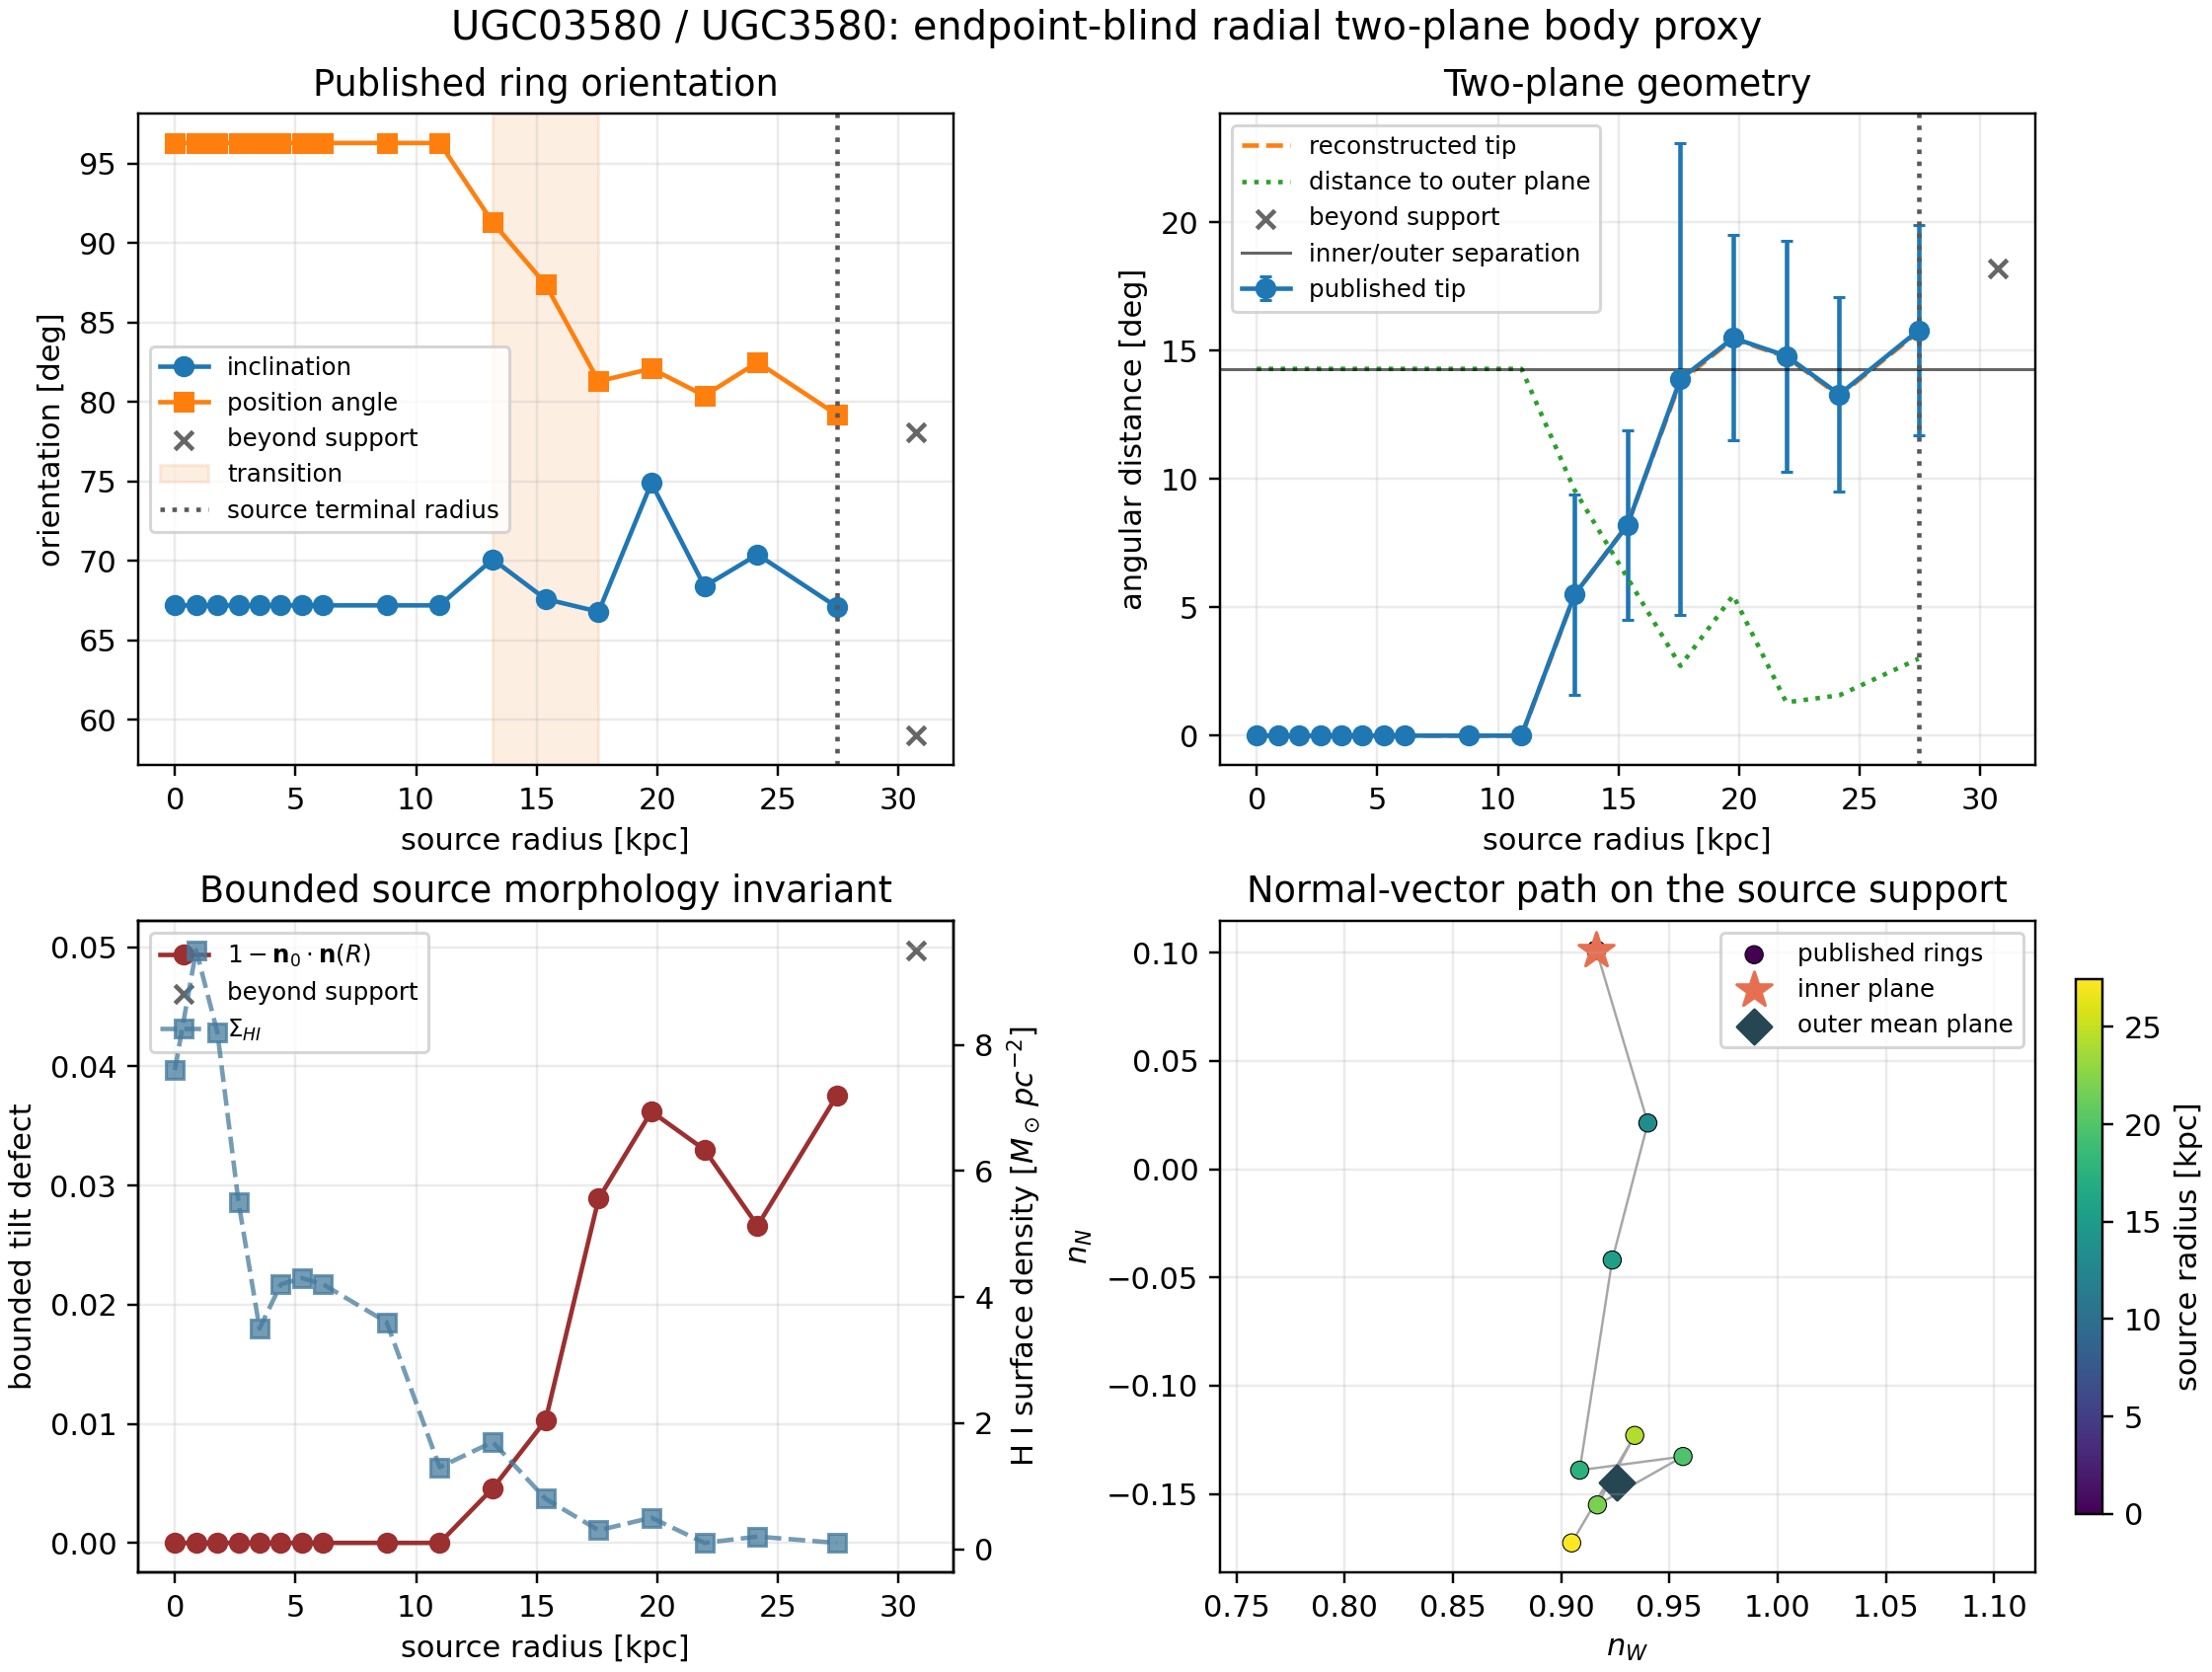
\includegraphics[width=0.98\linewidth]{figures/fig_ugc03580_ugc3580_two_plane_body_v01.png}
\caption{Endpoint-blind UGC03580/UGC3580 radial morphology refinement.  The
upper panels show the published ring orientation and its separation from the
source-defined inner and outer planes.  The lower panels show the bounded tilt
defect, H~I support and the normal-vector path.  Crosses lie beyond the source
terminal support and do not enter the primary outer-plane estimate.}
\end{figure}

This construction closes a source-representation defect: UGC03580 is no
longer reduced to one onset number.  It does not repair the failed endpoint,
select a bounded readout law, or show that warp geometry explains the rotation
curve.  In Tau Core terminology it is a localized galaxy-scale descriptor of
a downstream subsystem, not a separately seeded universe-level
morphological body \(M_\tau\).  A bounded two-plane terminal shell remains a
new source-side hypothesis and must be frozen before a genuinely new endpoint.

\subsection{Bounded two-plane coordinate and terminal non-identifiability}

The radial body is sufficient to define a bounded morphology coordinate, but
not a unique physical readout.  Let \(\mathbf n_{\rm in}\) and
\(\mathbf n_{\rm out}\) denote the source-defined reference planes and set
\[
d_{\rm in}(R)=1-\mathbf n_{\rm in}\!\cdot\!\mathbf n(R),
\qquad
d_{\rm out}(R)=1-\mathbf n_{\rm out}\!\cdot\!\mathbf n(R).
\]
For any \(p>0\), define
\[
K_p(R)=
\frac{d_{\rm in}(R)^p}
     {d_{\rm in}(R)^p+d_{\rm out}(R)^p}.
\]
Both defects are nonnegative.  For distinct reference planes their powers
cannot vanish simultaneously, hence
\[
0\leq K_p\leq1,\qquad
K_p(\mathbf n_{\rm in})=0,\qquad
K_p(\mathbf n_{\rm out})=1.
\]
Exchanging the plane labels gives exactly \(1-K_p\).  If the two reference
planes coincide, we define \(K_p=0\), because no active two-plane morphology
then exists.  These statements are algebraic consequences of the frozen body.
The choice \(p=1\) is only the minimal affine-defect convention; the source
does not select it physically.

The remaining ambiguity can be proved constructively.  For every
\(p>0\), \(0\leq a\leq1\), \(s\in\{-1,+1\}\), and nonnegative carrier
\(v_{\rm c}^2(R)\), the family
\[
v_{p,a,s}^2(R)=v_{\rm c}^2(R)\,[1+s\,aK_p(R)]
\]
is dimensionally valid and nonnegative and recovers the carrier when
\(K_p=0\) or \(a=0\).  Different \(p\), \(a\), or \(s\) generally produce
different terminal curves while sharing the same source body.  Thus the
two-plane morphology alone cannot determine the terminal exponent, amplitude,
sign, carrier, or physical occupation.  This is an explicit non-identifiability
counterfamily, not a failed numerical fit.

For UGC03580, the plane separation gives the source-only diagnostic scale
\[
a_{\rm sep}=\frac{1-\mathbf n_{\rm in}\cdot\mathbf n_{\rm out}}{2}
=\sin^2\!\left(\frac{\Theta}{2}\right)
=0.015484869.
\]
On the supported rings, \(K_1\) ranges from \(0\) to \(0.992276495\), while
the largest transition-zone difference between \(K_1\) and \(K_2\) is
\(0.149874019\).  The envelope
\(v_{\rm c}^2[1\pm a_{\rm sep}K_1]\) is therefore retained only as a
geometry-scale control; no source theorem identifies \(a_{\rm sep}\) with a
physical coupling.

There is also an exact standard-geometry control.  If a circular ring with
inclination \(i(R)\) is reduced using the fixed inner inclination \(i_0\), its
inferred squared speed is multiplied by
\[
G_{\rm proj}(R)=\left[\frac{\sin i(R)}{\sin i_0}\right]^2.
\]
The supported UGC03580 range is \(0.994090714\)--\(1.096849451\).  This factor
is not Tau-specific and is applicable only if the terminal reduction actually
used the fixed inner inclination.  It must therefore be audited as a standard
projection null before any morphology-readout claim.

The endpoint-blind construction and independent audit pass all declared
checks without reading a rotation endpoint.  The resulting status is
\texttt{FORMULA\_SHELL\_DERIVED\_ENDPOINT\_BLOCKED}: a bounded morphology
coordinate is derived, but terminal scoring remains inadmissible until a
parent/source law independently freezes the body registration, complete
coupling, gravity/observer calibration, and projection applicability.

This blocker can be stated more exactly using the source-action response
theorem.  After the body has been solved and frozen, let \(Z_*(K)\) be the
regular post-body state, \(H_Z>0\) its reduced Hessian,
\(B_{ZK}=D_ZD_K\mathcal A_{\rm post}\) the source/body--response mixed block,
and \(L_G\) the typed gravity-terminal covector.  The implicit-function theorem
then gives
\[
D_KZ_*=-H_Z^{-1}B_{ZK},
\qquad
\Gamma=-L_GH_Z^{-1}B_{ZK},
\qquad
\delta v_G^2(R)=[\Gamma K](R).
\]
Coercivity of \(H_Z\) establishes a regular stable response but does not fix
the sign or normalization of \(B_{ZK}\), \(L_G\), or their contraction.  In
particular, replacing \(B_{ZK}\) by \(-B_{ZK}\) or by
\(\lambda B_{ZK}\), \(\lambda>0\), preserves the body and the positive Hessian
while reversing or rescaling the terminal response.  The executable audit
contains this same-body countermodel.

Moreover, the scalar shell above is a special factorized case, not the generic
consequence of the action response.  A radius-independent \(a\) exists only if
\[
\frac{[\Gamma K_p](R)}{v_{\rm c}^2(R)K_p(R)}=s\,a
\]
is constant on the nonzero support of \(K_p\).  Otherwise the correct local
law contains a radial response operator or gain function.  The exact exponent
\(p\) likewise requires the complete source-owned defect law to be
proportional to \(d^p\) on the support; the first nonzero analytic source jet
selects only a local leading order.  Finally, \(v_{\rm c}^2\) must be derived
as the calibrated zero-morphology physical terminal branch, not chosen as an
empirical residual baseline.

The existing common-action construction sharpens this list.  Let
$\widehat D=(d_{\rm in},d_{\rm out},\chi)$ be the complete signed descriptor
(the retention result is proved below), and let a source-owned, full-support
registration $I_{\widehat D}=\iota_{I\leftarrow\widehat D}(\widehat D)$ place
it in the Parent invariant used by one frozen JCSEL/BRAC plus
Einstein--Newton completion.  The chain rule then fixes

\[
B_{Z\widehat D}=B_{ZI}J_{I\leftarrow\widehat D},
\qquad
\Gamma_{\widehat D}=-L_GH_Z^{-1}B_{ZI}J_{I\leftarrow\widehat D},
\qquad
v_{\rm c}^2=O_G[Z_*(I_{\widehat D}=0)].
\]

Thus $B_{Z\widehat D}$, $L_G=D_ZO_G$, and the carrier are not three independent
gains inside that declared completion.  If $Z=(g,\varphi)$, exact
elimination of the occupied internal field gives

\[
H_G^{\rm eff}=H_{gg}-H_{g\varphi}H_{\varphi\varphi}^{-1}H_{\varphi g},
\qquad
B_{G\widehat D}^{\rm eff}=B_{g\widehat D}
-H_{g\varphi}H_{\varphi\varphi}^{-1}B_{\varphi\widehat D},
\]

and reproduces the complete response.  Dropping the internal-field Schur term
would therefore change the terminal rather than simplify the same law.

The remaining obstruction is upstream.  Two distinct Parent registrations
can have the same visible $K$ projection but differ along a terminal-visible
hidden direction.  The endpoint-free finite witness gives terminal gains
$-0.163083062345$ and $-0.136881148198$ for two such lifts, with exactly
zero visible-projection discrepancy; exact Schur reduction reproduces both.
Consequently the visible two-plane coordinate cannot reconstruct its own
Parent lift.  The expanded audit passes all 39/39 checks.  The current
source packet still does not derive the signed-descriptor registration, exact
full-support exponent/profile, any further full-Parent kernel safety, calibrated occupied
galaxy packet, or Nature-level selection of the common completion.  Endpoint
scoring remains blocked.

The hidden fibre can be characterized exactly for the source geometry rather
than left as an arbitrary Parent direction.  Let

\[
c={\mathbf n_{\rm in}\times\mathbf n_{\rm out}\over
\lVert\mathbf n_{\rm in}\times\mathbf n_{\rm out}\rVert},
\qquad
\chi(R)=c\mathbin{\cdot}\mathbf n(R).
\]

The raw pair $D=(d_{\rm in},d_{\rm out})$ fixes the projection of
$\mathbf n$ into the span of the two reference normals but generically leaves
the reflected pair

\[
\mathbf n_{\pm}=\mathbf n_{\parallel}
\pm\sqrt{1-\lVert\mathbf n_{\parallel}\rVert^2}\,c.
\]

They have equal $D$ and opposite $\chi$.  Conversely
$(d_{\rm in},d_{\rm out},\chi)$ reconstructs the oriented normal uniquely,
and

\[
\chi^2=1-p^TG_{\rm anchor}^{-1}p,
\qquad
p=(1-d_{\rm in},1-d_{\rm out})^T.
\]

This is a discrete fibre: away from $\chi=0$, $D:S^2\to\mathbb R^2$
already has local rank two.  Therefore a local Jacobian-null test cannot prove
terminal descent; every claimed terminal must be exactly equal on the mirror
pair, or $\chi$ must be retained in the shared descriptor.  On the supported
UGC03580 rings the source-only control spans
$-0.047813169\leq\chi\leq0.095201374$, includes both signs, and satisfies the
displayed identity with maximum independent residual below $2.4\times10^{-15}$.
The source resolves the quotient decision for the complete standard projection
stack.  Table~6 of J{\'o}zsa (2007) publishes the Cartesian components of the
oriented spin normal toward west, north and the observer, and the UGC3580
figure captions identify the approaching side as southeast
\cite{Jozsa2007WarpedDisks}.  Let $\ell$ be the line-of-sight unit vector and
$R_c\mathbf n=\mathbf n-2\chi c$.  For the standard fixed-inner-inclination
projection

\[
G_\ell(\mathbf n)
=\frac{1-(\ell\mathbin{\cdot}\mathbf n)^2}
{1-(\ell\mathbin{\cdot}\mathbf n_{\rm in})^2},
\]

direct expansion gives

\[
\boxed{
G_\ell(R_c\mathbf n)-G_\ell(\mathbf n)
=\frac{4\chi(\ell\mathbin{\cdot}c)
[(\ell\mathbin{\cdot}\mathbf n)-\chi(\ell\mathbin{\cdot}c)]}
{1-(\ell\mathbin{\cdot}\mathbf n_{\rm in})^2}.}
\]

This terminal is not mirror-even on the 17 supported rings.  The maximum
absolute difference is $0.142726674696$, the RMS difference is
$0.046534679366$, and the analytic identity residual is below
$2\times10^{-16}$.  At $R=270$ arcsec the source and reflected projections
are $1.096849451016$ and $0.954122776319$, respectively.  Consequently
$\chi$ must be retained in the complete descriptor for this lane.  This is a
standard projection and representation result; it is not evidence for
fundamental Parent handedness, a Tau-specific coupling to $\chi$, or a new
rotation effect.

The mixed-Hessian migration makes this standard control executable without
selecting a Tau correction.  For the Bregman graph registration of the complete
signed descriptor, $\Gamma=J_{OS}=D_{\widehat D}{\cal N}$, while the ordinary
projection terminal has covector
$P_R=(0,0,-2n_{\rm los}/\sin^2 i_{\rm global})$.  Hence

\[
 D_{\widehat D}G_{\rm proj}=P_RJ_{OS}.
\]

A source-only freeze using the published oriented ring normals and the SPARC
global distance and inclination fields verifies this chain rule to
$1.21\times10^{-10}$ without reading pointwise rotation velocities.  A
separate diagnostic scorer then applies
$v_{\rm pred}=\sqrt{G_{\rm proj}}v_{\rm carrier}$ to the already opened
47-point UGC03580 terminal.  The central-catalog RMSE changes are
$-0.617\,\mathrm{km\,s^{-1}}$ for Newtonian baryons,
$+3.102\,\mathrm{km\,s^{-1}}$ for TPG/v6, and
$+3.531\,\mathrm{km\,s^{-1}}$ for fixed MOND.  Their signs remain unchanged
over the declared distance/inclination uncertainty grid and linear/nearest
interpolation control.  Thus this ordinary projection sensitivity does not
explain the residual remaining after TPG/v6 or MOND in this galaxy.  This is a
post-open standard-systematics diagnostic, not a Tau endpoint.  If the
published terminal already contains the same tilted-ring correction, its
reapplication would be double counting.

The same construction has also been frozen prospectively at the source side
for NGC2541 (UGC4284), without reading a rotation-velocity endpoint. The
published oriented-ring geometry gives 25 supported rings over
$30$--$590$ arcsec. For
$\widehat D=(d_{\rm in},d_{\rm out},\chi)$ the frozen decoder is

\[
 \mathcal{N}(\widehat D)
 =A^{-1}(1-d_{\rm in},1-d_{\rm out},\chi)^{\mathsf T},
 \qquad
 J_{OS}=A^{-1}\operatorname{diag}(-1,-1,+1).
\]

Its basis condition number is $6.57269$, the maximum reconstruction error is
$8.40\times10^{-16}$, and the standard fixed-inclination chain-rule check
closes to $1.24\times10^{-10}$. The resulting reference projection ratio
ranges from $0.81865$ to $1.03107$, but remains a sensitivity diagnostic, not
a selected Tau correction. No endpoint values or fit parameters enter this
freeze. Its status is therefore source-geometry ready but terminal-calibration
and untouched-endpoint blocked; no score is reported.

We subsequently executed the frozen calibration protocol on independently
reduced HALOGAS DR1 high-resolution moment maps
\cite{Heald2011HALOGAS,Heald2019HALOGASDR1}. The protocol and runner were
hashed before endpoint access; the first execution stopped before producing
any statistic because the FITS WCS and fixed centre used different celestial
frames, and the lock records the sole coordinate-frame compatibility fix. On
23 common eligible rings, the variable source geometry changes the mean
approaching--receding side discrepancy from
$13.2069$ to $12.5729\,\mathrm{km\,s^{-1}}$, or
$-0.6341\,\mathrm{km\,s^{-1}}$, with no fitted parameter. A required nuisance
audit demotes this favorable direction: replacing the optical/NED centre by
the same source's fitted kinematic centre changes the delta to approximately
$+0.3799\,\mathrm{km\,s^{-1}}$; a four-arcsec eastward shift gives
$+0.0888\,\mathrm{km\,s^{-1}}$, so even sub-beam centre changes can reverse
its sign. Moreover, the fixed and variable reductions selected different sky
pixels, the 12-arcsec inner ring spacing is smaller than the
14--17.5-arcsec beam, and several accepted sides contain less than one
synthesized beam. The earlier ring-iid bootstrap interval and sign-flip
$p=0.2144$ are therefore naive descriptive diagnostics, not calibrated
population evidence. We classify this as a post-open moment-1 side-symmetry
diagnostic with unstable calibration, not a standard-calibration detection.
It neither selects a Tau-specific $q_R$ nor tests a dark-matter replacement.

This audit fixes the design of the next population test. NGC~2541 is a
development case and is excluded from confirmation. NGC~3198 is likewise
excluded because its diagnostic and replay scores were already opened, while
NGC~5055 is excluded because it belonged to the Paper~8 SPARC training
population. The galaxy is the
inference unit, every candidate geometry is evaluated on one common sky
footprint, and beam-block covariance, centre alternatives, source orientation
uncertainties, and numerical convergence are compulsory. Two galaxy-level
gains are frozen: improvement of the morphology geometry over fixed geometry,
and improvement over equal-complexity source-side wrong-family geometries.
Exact shared-sign permutations, a max-$T$ multiplicity control, and
leave-one-galaxy-out sign stability are required. This source-side protocol
freeze is not itself a population result or a physical $q_R$ selection.

An endpoint-blind audit of the checksum-verified 24-object HALOGAS DR1
manifest leaves eight moderate-inclination, previously unopened candidates
after these exclusions and the current edge-on cut are applied
\cite{Heald2011HALOGAS,Heald2019HALOGASDR1}. Thus HALOGAS alone is four
galaxies short of the frozen minimum of 12. NGC~925 was audited first. The
primary THINGS analysis publishes its centre, mean geometry, and adopted radial
inclination and position-angle curves \cite{deBlok2008THINGSRotation}. Both
curves are extracted from the immutable 561-by-756 source JPEG into 93
three-arcsecond rings over 15--291 arcsec. This corrects an earlier partial
freeze that treated the printed $66^\circ$ mean inclination as a constant
radial law. The digitized inclination and PA means are $64.861^\circ$ and
$286.608^\circ$, within $1.139^\circ$ and $0.008^\circ$ of the printed
summaries. The largest 90-percent raster-sensitivity widths are
$7.771^\circ$ and $4.195^\circ$ respectively; these are digitization
diagnostics, not physical covariance.

An independent THINGS fit supplies 15 orientation pairs with marginal errors
from 100-step residual-rescrambling Monte Carlo fits
\cite{Schmidt2016THINGSRadialGas}. That source also states that the geometry
inside $250''$ is non-identifiable because nearly solid-body rotation does not
separate inclination from rotation speed. At the only source-claimed robust
ring shared with the de Blok extraction ($270''$), the inclination gap is
$0.878^\circ$ (1.23 Schmidt marginal standard deviations), while the PA gap is
$3.773^\circ$ (2.91 such standard deviations). These ratios are diagnostics,
not cross-source significances, because de Blok physical errors, cross-ring
covariance and joint inclination--PA covariance are unavailable.

The six source-robust outer rings have at least 11.89 ideal projected
half-annulus beam areas even for the broadest published HALOGAS pilot beam, so
an outer-only route is not geometrically impossible before masking. It fails
the current clean-terminal source gate: the same outer disk is described as a
minor-merger gas stream with twisted isovelocity contours, warp/spiral
ambiguity and anomalous H\,{\sc i} \cite{Heald2011HALOGAS}. NGC~925 is
therefore retained only for a separately frozen disturbed-system robustness or
stronger-terminal lane, and NGC~4062 becomes the next clean source-acquisition
target. No HALOGAS endpoint pixel or score was opened in reaching this
decision. This remains a sampling and source-readiness result, not a physical
$q_R$ selection or Tau signal.

NGC~4062 was subsequently frozen and opened without changing that source-first
order. GHASP gives $i=68\pm2^\circ$, a receding
$PA=99\pm2^\circ$, and $v_{\rm sys}=758\pm1\,\mathrm{km\,s^{-1}}$
\cite{Epinat2008GHASPVI}. The independent HALOGAS 3DBarolo reduction gives
median $i=67.1^\circ$ and $PA=100.1^\circ$ and does not include NGC~4062
among the six discs it flags as substantially warped
\cite{Marasco2019HALOGASEPG}. Two non-overlapping LR-beam-sized common rings
were therefore frozen at $42''$ and $84''$, with HR as primary, LR as mandatory
replication, and centre, $i\pm5^\circ$, $PA\pm2^\circ$, and both published
systemic velocities as compulsory nuisance variants. The opened cross-tracer
side-odd contrast is consistent with zero: the HR GLS mean is
$4.27\pm10.23\,\mathrm{km\,s^{-1}}$ ($p=0.470$), and the LR mean is
$3.22\pm10.50\,\mathrm{km\,s^{-1}}$ ($p=0.556$). Their primary signs agree,
but changing from the HALOGAS catalogue velocity of $769\,\mathrm{km\,s^{-1}}$
to the GHASP value reverses the inferred sign in both resolutions. Hence the
confirmatory endpoint fails rather than supporting a nonzero readout effect.
After importing this result and the published interaction, warp, complexity,
and beam-smearing flags for the other seven moderate-inclination unopened
objects, the current HALOGAS pool contains no further clean candidate under
this protocol. Expansion must therefore use an independently source-frozen
survey family or a newly preregistered, stronger terminal; post-open repair of
NGC~4062 is forbidden.

The resulting calibration obstruction can nevertheless be stated exactly for
future work.  Let \(d\in\mathbb{R}^n\) be a radial contrast, let \(C\) be its
positive-definite covariance, and let the columns of \(G\) be source-frozen
nuisance tangents, including the velocity-zero-point direction. Then the
covariance-weighted residual maker
\[
 P_\perp=I-G(G^T C^{-1}G)^+G^T C^{-1}
\]
obeys \(P_\perp G=0\), \(P_\perp^2=P_\perp\), and
\(P_\perp(d+G\eta)=P_\perp d\). Thus it removes the declared additive
nuisance without fitting the endpoint signal. The construction also exposes
an identifiability condition: a target template \(s\) survives only when
\(\operatorname{rank}[G,s]=\operatorname{rank}G+1\). If both \(G\) and \(s\)
are the common two-ring vector, the entire putative signal is removed. A
post-open audit of NGC~4062 leaves only one of two radial degrees of freedom
and retains \(9.11\times10^{-4}\) (HR) and \(2.52\times10^{-5}\) (LR) of the
covariance-weighted information in a constant radial template. Its projected
diagnostic remains consistent with zero, but this is not a new confirmatory
score: the secant nuisance tangent was itself estimated from the two opened
systemic-velocity reductions. A new survey must therefore freeze a
source-owned or independently calibrated \(G\), covariance, target template,
rank tolerance, and minimum retained-information rule before opening the
contrast.

The already opened, independently sourced NGC~3726 GHASP--Ursa Major
development case provides a six-radius method control. Under its published
fixed-systemic-velocity side convention,
\(dO_t/dv_{{\rm sys},t}=-2\), so the two tracer zero points span only one
constant radial nuisance direction. The same covariance-weighted projector
therefore leaves five shape degrees of freedom. All operator identities pass,
and the projected statistic equals the previously reported residual about the
best constant, \(\chi^2=9.1784\) for five degrees of freedom
(\(p=0.1022\)); the shape-only zero null is not rejected. This closes the
constant-zero-point algebra in that fixed-side model but not the physical
endpoint: a constant radial signal is annihilated, beam/centre/PA and radial
covariance remain incomplete, and no nonconstant morphology template has been
source-frozen on an unopened sample.

A further residual-blind sensitivity control found a previously missed
machine-readable Ursa Major side table for the interacting system NGC~3893.
Before reading its velocities, four common radii
\((20'',40'',60'',80'')\), the literature disturbance onset above \(75''\),
the nonconstant template \((0,0,0,1)\), and the same zero-point projection
were frozen. The opened matched amplitude is
\(7.78\pm11.40\,\mathrm{km\,s^{-1}}\) (\(p=0.495\)); the full projected
shape statistic is \(\chi^2=0.964\) for three degrees of freedom
(\(p=0.810\)). Thus this terminal does not detect even the predeclared
conventional disturbed-system control. Because the source literature analysed
related kinematics, this was never an independent Tau endpoint; its negative
result instead weakens the demonstrated morphology sensitivity of the current
side-odd instrument. No post-open template, radius or covariance repair is
made.

We also froze an independent two-dimensional H I sensitivity control on an
exact three-disturbed/three-quiet VIVA cohort \cite{Chung2009VIVA}.  The
operator uses the standard harmonic projection fact that an in-plane
morphology mode $m$ contributes to line-of-sight velocity sidebands
$k=m-1$ and $k=m+1$, consistent with nearby-galaxy Fourier velocity-field
practice \cite{Salak2019COMING}.  For the frozen $m=1$ construction the
lower sideband overlaps the nuisance sector, so the test retains the two
quadratures of $k=2$, with four preregistered annuli, held-out azimuthal
sectors and three wrong-template controls.  After cube opening, every galaxy
failed the frozen requirement of at least 24 beam-independent samples and
eight occupied sectors in every annulus (total retained sample counts
$29,4,81,28,27,45$).  The pipeline therefore emitted no velocity score and
the opened cohort is not repaired post hoc.  This is a resolution/capacity
failure of this implementation, not evidence against Tau, a parent-loss
measurement, a rotation correction or a dark-matter alternative.

We therefore preregistered a higher-resolution successor on the public LITTLE
THINGS H I products \cite{Hunter2012LITTLETHINGS,Holwerda2013HIMorphology}.
The source intake used the full 40-object table intersection rather than
disturbed/quiet labels. Twenty-five robust-weighted moment-0 maps survived the
catalogue geometry/support screen, 22 passed the image-level source-support
gate, and velocity-blind rank/injection calibration retained 20. Two objects
were excluded because one held-out azimuth block supplied no target novelty.
Before velocity access we also removed an invalid negative control: for a
two-quadrature target a global phase rotation spans exactly the same subspace.
The valid replacement applies a nonconstant annular phase scramble.

The frozen 20-galaxy moment-1 endpoint is negative. Matched-minus-best-wrong
specificity has mean $-0.107551$, median $-0.056207$, positive fraction $0.25$,
and exact one-sided sign-flip $p=0.983505$. No individual wrong-template
family yields a significant matched advantage, and all leave-one-galaxy-out
primary means remain negative. Thus the concrete same-tracer
$m=1\rightarrow k=2$ terminal does not demonstrate morphology-specific
kinematic sensitivity on this sample. The result weakens this terminal, not
the full parent/channel architecture: conventional lopsided gas dynamics,
tidal response, feedback, projection, and shared moment-map construction remain
sufficient alternatives. It is not a Tau detection, parent-loss measurement,
rotation correction, gravity result, or dark-matter replacement.

This endpoint is an auxiliary source-terminal sensitivity control, not the
primary test of observer-centred parent-distance loss. The latter requires a
separately derived observer--emission-point corridor
$\mathfrak C_{O\leftarrow x}$, its parent transfer $T_{P|Ox}$, and a frozen
observer access, noise, quantization, and calibration chain. Neither projected
galactocentric radius nor the H I $m=1$ mode is a substitute for that object.
The present negative score therefore neither tests nor weakens the open
corridor-loss hypothesis.
The four-image, two-transition SDP.81 program below is structurally closer
because it holds one source behind several lens paths. The conditional
Hessian-to-depth compiler is now derived, but no physical occupied parent
Hessian or path lift is present. Its current lens/source diagnostics are
therefore not yet a Tau parent-loss score.

An endpoint-free standard comparator has now been constructed from the frozen
Inoue smooth-lens model. For all four q1 paths it records relative Fermat
potential, the local lens Jacobian and its singular values, signed
magnification, and parity without reading a spectral or velocity endpoint.
All seven algebraic/provenance checks pass; the relative Fermat span is
$0.743341\,\mathrm{arcsec}^2$, the absolute magnification range is
$3.730$--$17.887$, and the centered path descriptor has rank three. These are
standard lens/corridor nuisance and comparison variables, not Tau parent
distance. Endpoint authorization remains false until a source-owned physical
$T_{P|Ox}$, parent-depth calibration, full covariance, and stable observer
terminal are independently frozen.
The largest q1 lens-Jacobi singular value is $1.038708$, one path therefore
exceeds unit operator norm, and two paths reverse parity. Together with the
different angular-coordinate domain, this forbids identifying the standard
lens Jacobian itself with the positive-metric parent-loss contraction; it
remains part of the conventional comparator.

The parent-loss generator is now frozen before any SDP.81 endpoint access.
Under the explicitly conditional post-body row-refinement principle
PCRR-P1, continuity, row locality and the inherited local half-unit uniquely
select
\[
 \Gamma_e={P_eK_{\rm src}P_e^*\over 2A_*\ell_*}.
\]
The accompanying theory audit passes all fourteen checks: square and
saturating spectral filters fail same-mode row-splitting invariance even
though they pass ordinary direct-sum naturality, while a quadratic source
Hessian alone still permits alternative positive stage metrics. Forward
decision PCRR-D1 therefore treats the linear law as the primary conditional
family and predeclares those alternatives as wrong-family controls. Endpoint
failure may demote this completion but may not select a replacement filter.
Physical parent depth, registration/orientation, source overlap, terminal
visibility and stable-cell crossing remain required before scoring is
authorized.

In the common commuting-mode branch this frozen choice gives a concrete
nuisance-reduced multipath invariant. If the corrected positive amplitudes are
$z_{in}=c_i s_n\exp(-\eta_i\lambda_n/2)$, double-centering $\log z$ over
paths and modes cancels arbitrary common source-mode amplitudes, path-scalar
gains, and the additive depth origin. The remainder must be
\[
 -{1\over2}(\eta_i-\bar\eta)(\lambda_n-\bar\lambda),
\]
and therefore has rank one. The theory audit passes all twelve checks. Rank
one alone is not a Tau signature: nonlinear spectral filters share it, while
path-and-mode-dependent differential magnification, beam, radiative-transfer,
or calibration terms survive. A future SDP.81 score must test alignment with
the full frozen outer product after those conventional terms, not merely low
rank.

The absolute scalar parent-distance unit is therefore not an eligibility
requirement for the first dimensionless score. If a source-side positive
parent interface Hessian supplies an invertible contraction $C_\gamma$, the
integrated morphology-depth operator
\[
 \Omega_\gamma=-\log[(C_\gamma C_\gamma^*)^{1/2}]
\]
and the polar orientation are unique and sufficient. A separate factorization
$\Omega=\eta F$ is not identifiable. Within PCRR-D1, a scalar $\eta$ is
admissible only if $\Omega$ lies exactly on the registered $K_{\rm src}/A_*$
ray; the twelve-check theory audit recovers its coefficient and rejects an
off-ray control. Consequently the remaining SDP.81 blocker is the physical
source-owned parent interface Hessian/transfer and its occupation, not an SI
calibration of parent length.

The ordered segment product is itself conditional. It follows from one
source-owned simultaneous innovation action with primitive residuals
$x_e-V_ex_{e-1}$; its triangular stationary solve yields $V_N\cdots V_1$
without introducing parent time. Generic positivity does not imply this law.
An additional positive internal susceptibility changes the endpoint transfer
and must be retained by exact Schur elimination. The supporting audit passes
all twelve checks. Thus the SDP.81 source freeze must supply either this
innovation factorization or the complete global corridor Hessian; multiplying
local contractions is otherwise unauthorized.

The missing transfer formula is nevertheless conditionally closed by the
existing FULLCONE body law. After all coupled corridor-interior morphology is
eliminated from one positive causal-body Hessian, split its positive boundary
Schur operator into source and observer blocks and define
\[
C_\gamma=-S_{OO}^{-1/2}S_{OS}S_{SS}^{-1/2}.
\]
A second Schur complement proves strict contraction, and the corresponding
theory audit passes all twelve checks. Paper 8 therefore no longer lacks a
mathematical $H_{\rm corridor}\mapsto C_\gamma$ map. It lacks physical source
selection and occupation of that causal-body Hessian, together with a
source-owned co-registration between the four optical SDP.81 paths and four
complete parent-corridor restrictions. Those objects must be frozen before
spectral pixels are read.

CSCR-T32h/PATHLIFT-C1 makes this co-registration condition exact. An occupied
EBOA parent path already fixes its restriction and observer trace, but one
observed 4D ray fixes a unique FULLCONE transfer only if that transfer is
constant, up to canonical endpoint-frame isometries, over the entire fibre of
parent lifts above the ray. Positive same-ray countermodels yield different
transfers and integrated morphology depths. The source-only SDP.81 audit
passes all eight method checks and supplies four unique optical path keys without
reading spectral pixels, but materializes none of seven physical lift
requirements. Neither a common occupied parent-Hessian key with a
fibre-basicness certificate nor four occupied parent-lift keys under one such
packet is present. The result is therefore \texttt{PREFLIGHT\_NOT\_ENDPOINT};
standard Fermat potentials, parities and lens Jacobians cannot select the
missing parent lifts.

CSCR-T32i turns the fibre-basicness branch into an executable local
certificate. On every connected regular parent-lift fibre, the
endpoint-frame-covariant vertical derivative of $C_\gamma$ must vanish. It is
computed source-forward from the occupied Hessian jet by differentiating the
interior Schur complement and solving the Sylvester equations for the inverse
positive square roots. Disconnected fibres additionally require matching
component anchors. The twelve-check theory audit verifies these identities,
but the SDP.81 packet contains no occupied smooth parent-Hessian family,
$D\pi_{4D}$, vertical kernel or fibre-topology certificate. The required source
schema is sharper, while endpoint status remains unchanged.

CSCR-T32j gives a finite reduction only if the occupied parent packet supplies
a connected Lie-group action transitive on every regular lift fibre. Its
fundamental generators must span the complete vertical kernel at every orbit
point, and the endpoint-frame-covariant transfer defect must vanish on every
generator. A one-point check, a partial generator list, or an
identity-component calculation is insufficient; discrete components and
discrete isotropy require separate anchor or holonomy checks. The SDP.81
packet contains neither this group action nor occupied generator jets, so the
refinement leaves \texttt{PREFLIGHT\_NOT\_ENDPOINT} unchanged.

CSCR-T32k--T32l close the next source-side fork. A physically occupied,
fibre-transitive action that preserves the complete typed parent Hessian up to
one common positive scale is sufficient: Schur functoriality makes
$C_\gamma$ basic and the scale cancels. Hessian positivity does not construct
that action. A reconstruction must own a separately typed lift-space metric,
solve the vertical symmetry algebra of the complete packet, prove complete
flows, and obtain an everywhere-zero generator-span projector defect. The
standard two-dimensional lens-potential Hessian is not the parent Hessian,
$d\beta/d\theta$ is not $D\pi_{4D}$, four-image multiplicity is not parent
fibre topology, and an optical path key is not an occupied parent-lift key.
None can be promoted by relabelling, so endpoint status remains closed.

The minimum-scope physical acquisition is consequently the direct-lift route:
one common physical parent-Hessian/selector-law packet, independently reviewed
source ownership, typed $E_P\to E_{4D}$, and one nonzero positive actual
post-body observer--source incidence measure. The four parent-lift keys must
then be derived by pushing that measure through the common selector, with
$\pi_{4D}(\widetilde\gamma_i)=\gamma_i$ certificates, frozen before any
spectral endpoint read. A manifest hash proves record integrity rather than
physical occupation.

CSCR-T32m--T32n prove that the keyed route is mathematically nonempty without
promoting it to physical occupation. A fibre-proper, strongly convex post-body
selector gives a unique smooth conditional section, and the selected positive
$S/O/I$ Hessian gives the strict FULLCONE transfer. A simultaneous mixed
body/lift scalar action is inadmissible because it backreacts on the frozen
body. Gauge-invariant uniqueness is only orbit uniqueness unless a separate
source-owned slice is supplied. The 23-check theory audit constructs four
conditional keys but leaves Nature occupation false.

CSCR-T32o--T32q remove one redundant occupation layer. Given a physically
realized selector law and actual positive observer--source incidence, the
occupied-lift measure and four keys follow by pushforward rather than as four
independent facts. Actual 4D paths alone do not select the parent section. The
least exact local occurrence law is the section graph square, with zero
upstream Schur remainder, so it cannot refit the frozen body. The 20-check
theory audit verifies the conditional identities; SDP.81 supplies neither
physical selector-law ownership nor parent-lift occupation.

The observed 4D incidence statement is now stronger. An endpoint-blind audit
of fixed $0.12$ arcsec apertures in the ALMA Band-7 continuum image detects all
four registered q1 locations above both integrated and peak $5\sigma$
thresholds. The integrated SNR range is $21.061$--$29.729$ and the peak range
is $10.434$--$13.553$. This supplies a positive, unweighted 4D counting measure
of mass four, not a parent-lift measure. It does not select the physical parent
section, so the physical count remains zero of seven and the endpoint remains
closed.

CSCR-T32s--T32u make the remaining selector request finite. One physically
owned complete post-body action would derive the selector, its Schur Hessian
and section jet by exact elimination. In the linear positive-action class the
unique coefficient-free candidate is

\[
J_{\min}=H_P^{-1}L^*(L H_P^{-1}L^*)^{-1},
\qquad K_{\min}=H_P|_{\ker L},\qquad L=D\pi.
\]

The two theory audits pass 15/15 and 14/14 checks. The current source domain,
however, has no parent-path fibre map or physically owned affine parent
anchor. A vertical affine shift preserves the entire observed 4D packet while
selecting a different parent lift. PLMIN-P1 is therefore selected only
conditionally inside its declared class; the physical gate remains zero of
seven.

CSCR-T32v--T32w require the lift selector and the $S/O/I$ transfer to descend
from one source-owned post-body action rather than from separately entered
Hessians. Nested Schur elimination derives the effective lift metric and the
boundary transfer without double counting. It also distinguishes a
source-selected lift held fixed under terminal variation from a lift that
relaxes jointly with that variation. The two boundary Hessians differ by a
positive-semidefinite Schur term for nonzero effective coupling, and the
normalized transfers generally differ, so
this semantics must be source-frozen before endpoint access. The 16-check
theory audit proves the identities, but no current SDP.81 artifact owns the
common action, correctly typed affine path descent, anchor or Nature
occupation. The physical gate therefore remains zero of seven.

The corresponding scoring path is now executable and fail-closed. A
source-only compiler reduces each authorized pathwise $(B,u,I)$ Hessian to the
selected fixed-lift or relaxed-lift transfer, freezes a five-dimensional
centered-log spectral terminal and pathwise covariance, and declares a
leave-one-path-out common-source statistic. Three paths reconstruct one latent
source-mode vector and predict the fourth. Lossless identity transfer and all
wrong path-to-transfer assignments are frozen controls. A separate endpoint
runner is the only component permitted to open the CO(8--7) cube. With no
physical manifest, both stages return
\texttt{FORMULA\_SHELL\_DERIVED\_ENDPOINT\_BLOCKED}; the endpoint-read flag is
false and no score is emitted. Seven targeted tests verify authorized
synthetic compilation, source recovery, wrong-assignment discrimination,
common-gain invariance,
nested-Schur positivity, foldwise source identifiability and perturbation
stability.

Any eventual score on this SDP.81 cube remains retrospective because its
spectral values were inspected before the common-action formula freeze. It
may serve as an informative diagnostic but not as a novel prediction. A
confirmatory test requires a new untouched same-source multipath endpoint.

We nevertheless execute one explicitly nonphysical sensitivity control.  The
conventional relative Fermat coordinate is retained in its 4D comparator type,
normalized to $r_i\in[0,1]$, and mapped through the unit-normalized path-graph
Laplacian $K$ of the six ordered spectral channels,
$C_i=\exp[-(1+r_i)K]$.  This formula has no fitted coefficient and is frozen
before the spectral values are reread, but it is not identified with parent
distance or a Nature-occupied Tau action.  Its held-out identity-metric
quadratic sensitivity is $4.46913$, slightly worse than the lossless value
$4.35135$; it does not beat the wrong-path-assignment median, and 17 of the 23
nonidentity assignments are no worse.  We therefore retain
\texttt{FIXED\_4D\_PROXY\_NOT\_PREFERRED} as a negative retrospective
diagnostic.  Since the identity covariance is not a measured noise
covariance, these values are not calibrated chi-square statistics.  The
result rejects only this fixed 4D proxy family, not the broader parent-loss
hypothesis.

A second diagnostic propagates channel covariance measured from fixed blank
aperture grids into the centered-log modes. Across nine annulus/grid
geometries the matched proxy beats the lossless model in six and the
wrong-assignment median in all nine, but it beats every wrong assignment in
none; between $39.1\%$ and $47.8\%$ of wrong assignments remain no worse.
Moreover, the frozen unit strength is the descriptive grid optimum in only
two geometries, whereas strength $0.5$ is optimal in seven. Post-endpoint
retuning is forbidden. Thus covariance weighting changes the result from a
simple negative norm comparison to weak path-order compatibility, but not to
model selection or physical evidence.

We next freeze a source-constrained diagnostic rather than fitting that
post-endpoint scale.  The independently pre-existing conditional
CSCR-T32c/PCRR-D1 refinement rule fixes the linear generator factor to one
half, giving
\[
C_i^{(\mathrm{PCRR}|4D)}=\exp[-(1+r_i)K_{\rm ch}/2].
\]
Across the same nine covariance geometries this candidate beats lossless in
nine and the wrong-assignment median in nine, but it beats every wrong
assignment in none; $34.8\%$--$39.1\%$ of wrong assignments remain no worse.
The exact rank p-values among all $4!=24$ assignments are $0.375$--$0.417$,
and no geometry reaches $0.05$. These are conditional ranks under the
exchangeable path-label null, not population-level significance values.
We therefore record PCRR half-shape compatibility without identification.
This is a
retrospective intersection between a source-pre-existing conditional factor
and an already exposed endpoint, not a prediction: $r_i$ is still a
conventional Fermat proxy, not a derived parent distance.

A companion diagnostic inserts the WR-T19 five-mode stiffness spectrum
\[
H_C=\operatorname{diag}(1.25,1.5,2,2.5,3),
\]
normalized by its frozen maximum.
The increasing-stiffness alignment leaves only $4.3\%$--$30.4\%$ of wrong
assignments no worse and gives exact rank p-values $0.083$--$0.333$, but never
wins against every wrong assignment or reaches $0.05$.  The
eigenmode-to-Helmert-mode alignment is not derived and its reversal is retained
as a control.  It is therefore a terminal-calibration hypothesis, not a
physical source identification.  Both diagnostics leave the physical gate at
zero of seven.

A stricter follow-up removes the arbitrary ordering of the Helmert columns.
The six ordered channels define the path graph $P_6$. Its centered normalized
Laplacian has five simple eigenvalues, hence its eigenvectors provide a
canonical mode basis up to signs. Every self-adjoint terminal operator that
commutes with this Laplacian is diagonal in that basis. This does not determine
which WR-T19 stiffness belongs to which graph frequency: every permutation of
the five stiffnesses still commutes. The predeclared monotone assignment gives
exact path-assignment rank $p=0.375$--$0.417$, while its reversed control gives
$0.083$--$0.333$ and an isotropic control gives $0.333$--$0.375$. No candidate
beats every wrong assignment or reaches $0.05$. We therefore derive the
canonical basis but do not support the monotone assignment. The better reverse
control is not promoted: this is a retrospective comparison using the same 4D
Fermat proxy, not a physical parent-to-terminal calibration.
Exhausting all $5!=120$ stiffness-to-graph-mode permutations places the
monotone assignment only at rank $39$--$81$ of 120
($p=0.325$--$0.675$) across the nine covariance geometries; the reverse ranks
$55$--$97$. Three different permutations are best in at least one geometry.
The endpoint therefore selects neither monotonicity nor a stable alternative
assignment.

The remaining calibration can be written without guessing another basis. A
source-owned post-body joint action gives
$W=-H_Z^{-1}B_{ZC}$. For each lensed path $i$, let $\Phi_i$ be the independently
sourced positive-flux composition of CO line formation, lens propagation,
instrument response, and aperture extraction. At a positive baseline $F_i^0$,
the logarithms use fixed positive same-unit flux references, which drop out on
differentiation. The local centered-log calibration is
\[
C_{{\rm ST},i}
=-U_0^\top\operatorname{diag}[(F_i^0)^{-1}]
 D_Z\Phi_i\,H_Z^{-1}B_{ZC}.
\]
Whitening this operator by the centered-log covariance and source metric and
taking its SVD defines the calibrated terminal and parent modes. The $P_6$
basis follows only when the resulting whitened terminal Gram commutes with the
graph Laplacian. Positive graph-aligned and rotated same-reduct completions
show that the present parent metrics, graph, and WR-T19 spectrum do not select
$B_{ZC}$ or the CO radiative port. The formula is therefore derived locally,
but the four physical path-specific Jacobians are absent and the endpoint
remains sealed.

The ordinary downstream part of those Jacobians can be factored more sharply.
Let $S_{nk}(Z)$ denote source-plane line emission in spatial basis cell $n$ and
channel $k$, and let $L_{in}$ be the fixed smooth-lens plus aperture response
of path $i$. Then
\[
 F_{ik}(Z)=\sum_n L_{in}S_{nk}(Z),\qquad
 [D_Z\Phi_i]_{ka}=\sum_n L_{in}[D_ZS]_{nka}.
\]
An endpoint-blind quadrature on the four registered q1 paths and the frozen
49-cell source basis gives a rank-four path matrix, leaving 45 spatial null
directions per channel. If $S_{nk}(Z)=p_n f_k(Z)$, each path differs only by a
scalar gain, which centered log channels cancel exactly; the maximum numerical
Jacobian spread is $3.69\times10^{-16}$. A nonseparable spatial--spectral
countermodel under the identical smooth lens gives spread $0.2869$ without
parent loss. Hence standard lens geometry is explicit, but a source-owned
CO(10--9) radiative mixed jet $D_ZS$, its line-specific instrumental response,
and covariance remain open. Spatial--spectral differential magnification is a
mandatory standard-physics control for any later parent-loss score.

The unresolved radiative jet admits a second exact local factorization,
$D_ZS=(D_\xi S)P$ with $P=D_Z\xi$. Standard molecular-line calculations take
gas temperature, density, column density, linewidth, and background radiation
as physical inputs \cite{vanDerTak2007RADEX,MangumShirley2015}; they determine
$D_\xi S$ only after the gas state and transfer closure are fixed, and do not
determine the cross-type map $P$. For a uniform slab,
\[
 S_k=\eta\,\Delta J\left(1-e^{-\tau_0\phi_k(v,w)}\right).
\]
Centered logs annihilate both multiplicative amplitude columns, leaving rank
at most three, or at most two in the optically thin limit. Thus one homogeneous
component cannot calibrate five modes. A two-component thin Gaussian mixture,
after common-gain quotienting, has relative amplitude, two centroid, and two
width coordinates. The endpoint-blind witness has rank five and minimum
singular value $0.231306$; coincident components collapse to rank two. This
proves only that a minimal radiative completion is nonempty. The source-owned
full-rank parent/body-to-gas bridge $P$, CO(10--9) gas baseline, line-specific
instrument response, and covariance remain open. The retrospective CO(8--7)
two-component preference cannot select them.

For the common-volume direction there is nevertheless one exact standard
transfer derivative. At fixed source function,
\[
 I_j=S_j(1-e^{-\tau_j}),\qquad
 \tau_j(\zeta)=e^\zeta\tau_j
 \quad\Longrightarrow\quad
 {\partial\log I_j\over\partial\zeta}\bigg|_0
 ={\tau_j\over e^{\tau_j}-1}.
\]
This positive response is strictly decreasing with positive optical depth.
Equal channel opacities, and the leading optically thin uniform gain, vanish
under centered logs; unequal opacities can survive as a line-shape mode
\cite{MangumShirley2015}. A varying source function contributes a separate
$\partial_\zeta\log S_j$ term.

The two already exposed transitions do not identify this derivative. For any
positive opacity pair and measured positive intensities, setting
$S_j=I_j/(1-e^{-\tau_j})$ reproduces the same observations while changing the
volume response. Two positive counterfamilies reproduce the published
intrinsic $r_{8-7/5-4}=0.30\pm0.04$ but yield different centered responses.
Moreover, the reconstructed CO(5--4) and CO(8--7) distributions are known to
have excitation-dependent morphology \cite{Rybak2015SDP81CO}. The expanded
endpoint-blind audit passes all thirteen checks and proves non-identifiability,
not a source freeze. Independent channel-wise excitation/source-function or
opacity information, with filling and differential magnification, remains
necessary before CO(10--9) can be scored.

We have now executed the source-acquisition part of that route using the
official 200-pc SDP.81 multi-line products \cite{Rybak2020FullOfOrions}, while
excluding CO(10--9) from both inputs and fit. A solar-metallicity
\texttt{wk2006} PDR fit to FIR, [C\,II], CO(3--2), CO(5--4), and CO(8--7)
has 288 pixels detected at S/N at least three in every tracer. Eighty pixels
have reduced $\chi^2<5$. The blind median CO(10--9)/CO(5--4) prediction is
$0.231$, with median relative 68\% half-width $0.363$; its median change
between 0.05-dex and 0.10-dex grids is 6.0\%, narrowly failing the frozen 5\%
stability check. This is therefore a partial integrated-amplitude prior, not a
channel-wise opacity certificate.

The distinction is exact. Write the source-cell emission as
$S_{nk}=A_np_{nk}$ with $p_n>0$ and $\sum_kp_{nk}=1$. A nonzero sufficiently
small perturbation $p_m\mapsto p_m+\epsilon h$, with
$\mathbf 1^\top h=0$, preserves all integrated amplitudes. For every path
with $L_{im}A_m>0$, however,
\[
 \delta F_i=\epsilon L_{im}A_mh,\qquad
 \delta y_i=\epsilon L_{im}A_m
 U_0^\top\operatorname{diag}(F_i)^{-1}h,
\]
which is generically nonzero. At derivative level,
$D_ZS_{nk}=(D_ZA_n)p_{nk}+A_nD_Zp_{nk}$ leaves the independent zero-sum
profile derivative unresolved. Thus the integrated PDR result cannot be split
into six channels by convention. A source-owned channel profile, its response,
filling and differential magnification remain required; an isotopologue or
other direct opacity tracer would be cleaner.

The available open products do not supply that missing lift. Their official
source reconstructions are two-dimensional velocity-integrated maps rather
than source-plane spectral cubes. The current image-plane inverse
reconstruction promotes none of six channel-common source fits, while its
three-path-to-fourth-path test improves only one of 24 folds and has median
predictive $R^2=-21.187$. The cross-transition projected rank also remains
unpromoted. We therefore reject simple inheritance of the CO(8--7) normalized
profile as a CO(10--9) profile. This rejects one candidate completion, not a
richer standard line-formation law or Tau Core.

The cross-type bridge can be reduced one layer further while preserving the
body-first direction.  Let $Z$ be an already solved and frozen post-body
response and let the gas state be the stationary section of a conditional
functional, $D_\xi\mathcal E_{\rm gas}(\xi_*(Z);Z)=0$.  If
$H_\xi=D_\xi^2\mathcal E_{\rm gas}>0$ and
$B_{\xi Z}=D_\xi D_Z\mathcal E_{\rm gas}$, the implicit-function theorem gives
\[
 P=D_Z\xi_*=-H_\xi^{-1}B_{\xi Z},\qquad
 \operatorname{rank}P=\operatorname{rank}B_{\xi Z}.
\]
This is an ordered conditional response, not a simultaneous body/gas
variation.  In a jointly varied symmetric quadratic action, eliminating
$\xi$ changes the upstream Hessian to
$H_Z-B_{\xi Z}^{T}H_\xi^{-1}B_{\xi Z}$ and therefore generically reselects
the frozen response.  The endpoint-blind audit verifies the implicit formula,
rank and conditioning bounds, finite differences, a singular control, and
nonzero backreaction.  A quadratic same-Hessian counterfamily realizes
arbitrary distinct bridges, so stability proves neither the physical
$B_{\xi Z}$ nor Nature occupation.  The remaining source object is the typed,
occupied conditional gas law at the frozen line baseline; CO(10--9) stays
sealed.  The terminal-registration validator now reproduces both
$P=-H_\xi^{-1}B_{\xi Z}$ and every pathwise
$D_ZF_i=(D_\xi F_i)P$; a directly asserted raw flux Jacobian fails closed.

The available symmetries do not select the remaining mixed derivative.  A
genuinely common source-owned group action would imply
$P\rho_Z(g)=\rho_\xi(g)P$.  The ordered $P_6$ reflection splits the centered
five-space into parity multiplicities $2+3$, leaving a
$2^2+3^2=13$ dimensional intertwiner space with distinct full-rank members.
A hypothetical standard $S_6$ action has scalar commutant, but it is not a
symmetry of the ordered graph, is not physically represented on the gas
tangent, and still leaves the susceptibility scale free.  Component exchange
is not a local stabilizer at a generic distinct-component baseline; its fixed
locus has centered-log radiative rank two.  The endpoint-blind audit passes
all fourteen checks.  Thus a common source representation/intertwiner and one
nonzero susceptibility anchor, or an independently derived nonsymmetric
interaction, remains necessary.

The proposed four-dimensional intermediate can be stated exactly, but only as
a conditional mediation theorem.  If a gauge-quotiented environmental
descriptor $e(Z)$ carries all dependence of the gas functional on the frozen
post-body coordinate, then
\[
 P=D_e\xi_*D_Ze=-H_\xi^{-1}B_{\xi e}D_Ze.
\]
For fixed $G=D_Ze$, an $R$ with $P=RG$ exists if and only if
$\ker G\subseteq\ker P$, equivalently $P=PG^+G$ after inner products are
fixed.  A scalar descriptor therefore transmits at most one mode and a
four-component vector at most four; the five-mode terminal requires mediator
and response ranks of at least five.  Conversely, full-column rank of $G$
makes bare factorization automatic and non-identifying.  More generally a
direct mixed derivative contributes
$P_{\rm dir}=-H_\xi^{-1}B_{\xi Z}^{\rm dir}$, so pure mediation additionally
requires a no-direct-coupling certificate.  The endpoint-blind audit passes
all thirteen checks.  No present artifact owns the physical descriptor,
$D_Ze$, $B_{\xi e}$, or that certificate.  The terminal gate now accepts only
a source-owned direct cross derivative or a reproduced gauge-quotiented
mediator packet; downstream lens/path geometry cannot be substituted for it.

The existing G4D branch supplies one concrete candidate mediator.  Introduce
a source-owned registration $I_{ZA}:T_Z\to X_A$ from the five post-body modes
to the observer--source input of the ordered G4D row.  Then
\[
 D_Zc_*=-L_C^{-1}D_C^*W_RD_AI_{ZA},\qquad
 D_Zh=J_{\rm met}D_Zc_*.
\]
At the GR leaf, $J_{\rm met}$ is an isomorphism from the ten metric-active
lapse, shift and symmetric-strain generators to the ten relative-metric
components.  On the unrestricted sixteen-component coframe tangent its kernel
is exactly the six-dimensional infinitesimal Lorentz algebra.  Hence an
abstract metric-only gas response with an access incidence of rank at least
five compiles without frame contamination as
\[
 P_{\rm cof}=-H_\xi^{-1}B_{\xi h}D_Zh.
\]
The updated endpoint-blind audit passes all fifty-six checks and constructs
an abstract rank-five witness.  It also constructs same-G4D countermodels: $I_{ZA}$ is not selected
by the G4D row, and $B_{\xi h}$ is not selected by the coframe response.  The
standard covariant matter mixed Hessian fixes the relevant variational type,
but not its reduction to the five phenomenological CO line coordinates.  The
physical G4D occupation, registration and gas--metric response remain open.

The registration need not remain a free matrix.  With the post-body $Z$
already frozen, one source-owned common relation codomain and typed rows
$R_Z:T_Z\to Y_{ZA}$, $R_A:X_A\to Y_{ZA}$ and $d_A:X_A\to Y_A$ give
\[
 I_{ZA}=-K_A^{-1}R_A^*W_{ZA}R_Z,
 \qquad K_A=R_A^*W_{ZA}R_A+d_A^*W_Ad_A>0.
\]
The common action scale cancels and rank-five transmission is equivalent to a
rank-five cross-Gram row.  The ordering is essential: a simultaneous symmetric
$Z/a$ solve produces the Schur correction
$B_{AZ}^*H_A^{-1}B_{AZ}$ in the already frozen $Z$ Hessian.  The permitted
lower-triangular response has zero access-to-$Z$ upper block and preserves the
body solution.  The endpoint-blind audit passes all fifteen checks.  It also
shows that an unsourced relation row can be chosen to reproduce an arbitrary
target registration, so the formula is not Nature selection.  The common
source codomain and occupied row blocks remain open, and CO(10-9) stays sealed.

The current concrete AORS specialization does not meet that rank premise.  Its
access star is
\[
 D_A^\star=(-\mathbf 1_4,I_4):\mathbb R^5\to\mathbb R^4,
 \qquad \ker D_A^\star=\operatorname{span}\{\mathbf 1_5\},
 \qquad \operatorname{rank}D_A^\star=4.
\]
It follows that $\operatorname{rank}D_Zh\leq4$ for every registration
$I_{ZA}$; the rank-ten coframe cannot restore a fifth mode already removed by
the access incidence.  The earlier rank-five construction is therefore an
abstract G4D compiler witness, not a realization by the current AORS packet.
The deficit is exactly one.  For the rank-four cross operator $T_0$, a scalar
shared row $uv^*$ raises the rank to five exactly when $u$ and $v$ lie outside
the current column and row images; a redundant row cannot.  Its distinguished
candidate direction is now fixed.  The normalized AORS common-null covector
$q_A=\mathbf1_5^*/\sqrt5$ pairs with the coframe determinant-line covector

\[
 q_V(\delta c)=D\log|\det D_O|_0[\delta c]
 =\delta\lambda+\operatorname{tr}\delta S
 ={1\over2}\operatorname{tr}(\eta^{-1}\delta h).
\]

The latter annihilates all six infinitesimal Lorentz gauge generators.  Thus
the natural mixed jet is $\gamma_{\rm cm}q_V^\sharp\otimes q_A$; after
registration it closes the deficit exactly when $\gamma_{\rm cm}\ne0$ and
both legs are transverse to the existing images.  Positivity of the scalar
source block gives only
$|\gamma_{\rm cm}|\leq\sqrt{k_Vk_A}$ and admits zero and both signs.  A
perfect-square source saturates the bound but still requires source-owned
diagonal susceptibilities and an orientation.  Including the correlated
coframe self-Hessian gives the exact ordered increment
\[
 \Delta R={L_0^{-1}u\over1+k_Vs}
 [k_Vu^*L_0^{-1}T_0-\gamma_{\rm cm}v^*],
 \qquad s=u^*L_0^{-1}u,
\]
which has rank at most one through metricization and any linear gas terminal.
In the single common relation-row class the coefficient is no longer
independent:
\[
 \gamma_{\rm cm}=\Lambda_A\langle D_Ce_V,D_Ae_A\rangle_{W_R}.
\]
Activation is therefore exactly nonzero, nonorthogonal occupation of the
coframe-volume and common-access relation images; their weighted cosine is
independent of the common action scale and their orientation fixes the sign.
The standard covariant matter variation further fixes the physical type of
the volume susceptibility. With
$T_{\mu\nu}=-(2/\sqrt{-g})\delta S_m/\delta g^{\mu\nu}$ and
$\delta g_{\mu\nu}=2\varphi g_{\mu\nu}$,
$\delta S_m=\int\sqrt{-g}\,\varphi T^\mu{}_{\mu}$ and $q_V=4\varphi$
\cite{Brown1993PerfectFluids}. Cold massive gas is generically traceful,
whereas classical radiation is a trace-free control. This does not force
five-mode visibility because centered logs remove uniform gain; the opacity
shape criterion above is still required.

The updated endpoint-blind audit passes all fifty-six checks, including
orthogonal, orientation-reversed, exact-cancellation and terminal-null
controls. Physical occupation, transversality, channel-wise opacity/excitation
and terminal registration are not supplied by the current source packet, so
the result does not open CO(10-9).

The same conditional family has a depth-free necessary consequence.  After
double centering over paths and channels, CSCR-T32d requires the log-spectral
interaction matrix to have rank at most one for commuting scalar-depth
transport.  This removes common source shape, pathwise scalar gain, and the
depth origin without identifying Fermat coordinate with parent distance.  The
observed singular values are $1.480641$, $0.411652$, and $0.293055$, so the
leading component contains $89.568\%$ of the double-centered energy.  Across
nine fixed covariance geometries, rank-zero noise gives an upper-tail
$p=0.140$--$0.163$, while the fitted-rank-one goodness-of-fit gives
$p=0.459$--$0.532$.  Neither model is rejected at $0.05$.  The result is
therefore rank-one compatible but not detected or identifying.  Nonlinear
separable filters share the same rank, and path-by-mode calibration can alter
it.

We also freeze the next prospective partial endpoint without opening it.  The
local Band-7 archive contains an unextracted CO(10-9) cube with frozen archive
hash and exact member name.  This is a held-out transition through the same
SDP.81 lens and source, not an independent-source replication.  The pre-pixel
gate passes all nineteen static archive, registration, incidence,
standard-path, radiative-rank, ordered parent--gas response, symmetry-no-go,
four-dimensional-mediator-boundary, G4D-coframe-compiler, blind integrated
PDR-amplitude and unsafe-profile-inheritance-rejection checks but zero of seven
parent-physical and one of six transition-readiness requirements. The seven
deterministically regenerated prerequisite hashes were explicitly re-frozen
before this count. The rejected profile shortcut now has an endpoint-blind
replacement route: official ALMA archive metadata separate 12 Band-4
CO(5--4) and nine Band-6 CO(8--7) executions (211.709 GB total) from all 11
Band-7 CO(10--9) executions. The permitted execution list and visibility-plane
reconstruction contract are frozen, but acquisition and source-cube
reconstruction have not occurred.  A resource-bounded first route instead
uses the two already-local restored CO(5--4)/CO(8--7) cubes, totaling only
395.928 MB, under a frozen full-arc, regularized, covariance-aware inversion
with held-path/channel/grid/beam controls.  That route is development-only
because restored images do not retain the full visibility likelihood. Neither
route therefore adds a transition-readiness item.  The resource-bounded
inversion has now been run: all four paths have positive median held-path
improvement, but the combined median is only $2.07\%$, below the frozen
$5\%$ threshold.  A fair reflected-source control reaches $1.61\%$, leaving
only a $0.46$ percentage-point matched advantage.  The restored-image family
is therefore not promoted and will not be tuned further.  Grid, beam,
astrometric and channel-block stability controls are not run after this
primary failure and cannot be claimed as passed.

The public reduced-product hierarchy is also now explicit.  The official
calibrated Band-4/Band-6 measurement-set packages total 54.009 GB, while the
1.599-GB reference-image tier contains the already-tested 395.928-MB pair of
allowed line cubes.  The public source-plane CO(5--4) and CO(8--7) products are
velocity-integrated maps rather than spectral cubes and do not supply a full
channel covariance or posterior.  No compact public source-plane spectral
likelihood or target-and-line-only calibrated visibility cutout was found.
The next finite action is therefore an author request for one of those compact
products; the 54.009-GB calibrated archive packages remain the smallest public
visibility fallback.  This inventory adds no transition-readiness item and
does not authorize access to the held-out CO(10--9) endpoint. Neither its FITS
header nor data array was read.  It remains sealed until a physical common-action packet and a
source-owned parent-mode-to-CO(10-9) terminal registration are frozen.

The source gate now reads physical authorization only from a separate,
artifact-verified physical manifest. Strings injected into the standard
corridor descriptor fail closed, and the direct route additionally requires
four explicit $\pi_{4D}(\widetilde\gamma_i)=\gamma_i$ certificates. A
hash-valid self-asserted manifest also fails unless it supplies the typed
post-body occurrence law, selector graph certificate, rival-lift control and
independent scientific review declaration. That
manifest is absent, all seven physical requirements remain false, and the
endpoint remains sealed.

There is also a sharp conditional selection of the scalar coordinate.  If the
registration is homogeneous of degree zero, affine on the normalized positive
two-defect simplex, and takes values zero and one at the inner and outer
anchors, respectively, then uniquely

\[
I_D=K_1={d_{\rm in}\over d_{\rm in}+d_{\rm out}}.
\]

The $K_p$ counterfamily shows that the limits, homogeneity and anchor-swap
law do not imply the affine premise.  Thus this theorem closes the local
geometry and normalized-affine class only; physical source ownership of that
class, its co-registration with the occupied JCSEL/BRAC invariant, calibration
and Nature occupation remain open.

The affine uniqueness statement does not make $K_1$ a complete descriptor.
It is constant on every raw-descriptor mirror pair, whereas the standard
projection above is not, so no single-valued $F$ can satisfy
$G_\ell=F\circ K_1$ on that support.  The frozen continuous source path gives
an independent within-path witness.  Bracketed solves on the disjoint
$210$--$240$ and $270$--$300$ arcsec shortest-great-circle segments give

\[
K_1=0.925
\quad\hbox{at}\quad
R=228.939929970\ \hbox{and}\ 275.245362641\ \mathrm{arcsec}.
\]

The corresponding signed coordinates are $-0.033824288698$ and
$+0.074850153783$, while the fixed-inclination projection values are
$0.998056542027$ and $1.084700249348$.  The projection difference is
$0.086643707321$.  Fixed neighboring levels $K_1=0.900$ and $0.950$ reproduce
the double intersection, with projection differences $0.093917224631$ and
$0.078771081452$, respectively.  The result is stable under the declared
bisection-tolerance control and uses no rotation endpoint.

Thus $K_1$ is not injective even on the frozen one-galaxy source path and
cannot replace the complete shared descriptor.  This does not prove that the
physical Parent coupling is multicomponent.  The range of $\widehat D$ is a
constrained two-dimensional surface, and a source-derived rank-one response
through another signed scalar remains logically possible.  Locally such a
collapse requires

\[
\Gamma_{\widehat D}=\gamma\otimes D_{\widehat D}u,
\qquad \operatorname{rank}\Gamma_{\widehat D}\leq1,
\]

plus the exact global terminal-fibre condition.  Positive post-body stability
does not imply this factorization.  Until it is independently derived, the
source-to-action handoff must retain $\widehat D$ or an exactly fibre-equivalent
descriptor. The historical expanded endpoint-free audit recorded 62/62
checks. A 15 September 2026 reproduction instead passes 61/62: the stored
chirality-square versus raw-defect identity fails its declared numerical
comparison, while the independent raw identity passes. The tolerance and
frozen source inputs have not been relaxed. Consequently full numerical
reproducibility of this shell is pending; it is not an accepted endpoint.

The retained descriptor also admits an endpoint-unfitted
complete-registration existence candidate without using the rotation
endpoint.  Let
$A_{ab}$ have rows
$(\mathbf n_{\rm in}^{T},\mathbf n_{\rm out}^{T},c^{T})$ and define

\[
\mathcal N(\widehat D)
=A_{ab}^{-1}
(1-d_{\rm in},1-d_{\rm out},\chi)^T.
\]

For a typed oriented-normal register $N$ and any positive source-frozen graph
metric $K_{\rm reg}$, the post-body action

\[
\mathcal A_{\rm reg}[N;\widehat D]
=\frac12
\langle N-\mathcal N(\widehat D),
K_{\rm reg}[N-\mathcal N(\widehat D)]\rangle
\]

has the unique zero-energy minimum
$N_*=\mathcal N(\widehat D)$.  On the physical descriptor surface the decoder
differential restricted to the descriptor tangent has rank two; the graph
metric changes the fluctuation cost but not the registered minimum or its
Jacobian.  This rank is complete
only for the signed two-plane oriented-normal sector, not for the whole
Parent or every physical interaction.

Because the exact decoder appears explicitly in the graph square, this is a
conditional existence and consistency construction.  It does not derive the
decoder or physical occupation from deeper Parent source primitives by
itself.

The inverse appearance can nevertheless be removed conditionally.  Define

\[
q(\widehat D)=(1-d_{\rm in},1-d_{\rm out},\chi)^T,
\qquad
\rho_{\rm TPORI}=A_{ab}N-q(\widehat D).
\]

If the post-body source owns this forward same-object incidence, then for
$W>0$

\[
\mathcal A_{\rm TPORI}
=\frac12\langle\rho_{\rm TPORI},W\rho_{\rm TPORI}\rangle
\]

has the unique zero
$N_*=A_{ab}^{-1}q(\widehat D)=\mathcal N(\widehat D)$ and is exactly the graph
action above with $K_{\rm reg}=A_{ab}^{T}WA_{ab}$.  Conversely every positive
$K_{\rm reg}$ determines one positive forward weight.  Thus the decoder is
derived from the forward incidence once that incidence is supplied.

Current source laws do not yet select it.  A smooth endpoint-blind,
proper-rotation-covariant twist of the oriented normal can fix the three
source-frame axes and retain rank two while defining a distinct positive
graph.  Hence positivity, covariance, anchor fixing, and complete local rank
do not force the same-object coidentity
$\widehat D_{ab}(N_*(\widehat D))=\widehat D$.  The separate endpoint-free
source-incidence audit passes 19/19 checks.  This is a conditional source-law
reduction and nonselection theorem, not physical occupation or an additional
Paper~8 empirical/source-shell check.

The physical meaning of the graph square is sharper still.  If $N$ merely
re-expresses the same descriptor, choose local descriptor coordinates $x$ and
register coordinates $u$, with decoder differential $u=Cx$.  Writing
$J_N=A_{ab}E_N$ and $Q=J_NC$, the linearized defect is

\[
\rho=J_Nu-Qx.
\]

Its positive-semidefinite joint Hessian has the decoder-graph tangent as its kernel, and
exact register elimination gives

\[
\boxed{H_{xx}-H_{xN}H_{NN}^{-1}H_{Nx}=0.}
\]

This is the local form of
$\min_N\mathcal A_{\rm TPORI}[N;\widehat D]=0$ for every admissible
$\widehat D$.  Hence a deterministic register adds no source rank, effective
descriptor stiffness, force, dark-sector term, or independent readout.  An
independently physical register would require a separately source-owned
off-graph load, typed mixed interaction, register-sensitive terminal, or
calibrated fluctuation spectrum.  The separate endpoint-free
Schur-neutrality audit passes 14/14 checks; current source ownership and
Nature occupation remain open.

The ordered downstream solve isolates the exact remaining linear target.
After $u_*=Cx$ is frozen, a response Hessian $H_Z>0$, mixed rows
$B_{Zu},B_{Zx}$, and de-duplicated indirect terminal $L$ give

\[
\boxed{
B_{\rm eff}=B_{Zu}C+B_{Zx},
\qquad
\Gamma_x=-LH_Z^{-1}B_{\rm eff}.}
\]

Nonzero register coupling alone is insufficient because the two rows may
cancel on the decoder graph; nonzero $B_{\rm eff}$ alone is insufficient
because the terminal may annihilate the solved response.  Replacing the
register path by the direct row $B'_{Zx}=B_{\rm eff}$ reproduces every
on-graph terminal exactly.  Register ontology therefore requires off-graph
fluctuations or an independently typed register-sensitive terminal.  The
separate endpoint-free no-bypass audit passes 15/15 checks.  Source ownership,
standard-comparator separation, and Nature occupation remain open.

The corresponding source-selection question can also be decided relative to
the current upstream reduct.  Keep the same frozen graph $u_*=Cx$, and let
$R:U\to Z$ be a typed post-registration incidence.  For $H_Z>0$, the
positive ordered family

\[
\mathcal A_Z^{(\lambda)}[z;u_*]
=\frac12\left\lVert z-\lambda Ru_*\right\rVert_{H_Z}^{2}
\]

has $B_{Zx}=0$, but its stationary response is

\[
z_*=\lambda RCx,
\qquad
B_{\rm eff}=-\lambda H_ZRC,
\qquad
\Gamma_x=\lambda LRC.
\]

Thus zero direct descriptor--response coupling does not imply zero indirect
mediation.  With the same descriptor, decoder and registration law,
$\lambda=0$, rank-one $R$, and full-rank $R$ realize response ranks zero,
one and two, respectively; changing the sign of $\lambda$ reverses the
response without violating positivity, and a nonzero $R$ may still be
annihilated by $L$.  The current source therefore selects none of activation,
rank, orientation, or terminal survival.  The separate endpoint-free
source-selection audit passes 18/18 checks.  A physical promotion requires a
typed endpoint-blind incidence and source-owned activation/orientation plus a
de-duplicated terminal satisfying $\lambda LRC\ne0$, followed by
standard-comparator separation and Nature occupation.  This is a conditional
non-emptiness and current-source non-entailment result, not evidence for a new
galactic force or dark-sector component.

A scalar JCSEL/BRAC descendant $I_K=f(N)$ instead obeys

\[
\operatorname{rank}
J_{I_K\leftarrow\widehat D}\leq1.
\]

Thus there is no contradiction between a rank-two complete shared register
and a rank-one scalar interaction.  The actual mixed block can still transmit
zero, one, or two directions.  Moreover, the pullback to the single radial
UGC03580 path has rank at most one, so this galaxy can reject a proposed
scalar fibre but cannot establish Nature-level rank-two occupation.  The
separate endpoint-free graph-action audit passes 22/22 checks; it is not
counted as an additional empirical/source-shell check.  Physical occupation
of this graph action and the map from $N$ to the scalar BRAC invariant remain
open.

\section{Negative-result taxonomy}

A poor score is not automatically a falsification of the morphology-readout
framework.  It must first be classified by source status.

\noindent\fbox{%
\begin{minipage}{0.94\linewidth}
\textbf{How to read a failure.}  A failed branch says that one formula family or
one component is insufficient.  A weak negative says that the current
morphology/source manifest is not strong enough to decide.  A true negative
requires a source-complete morphology manifest, a residual-blind frozen readout
family and amplitude rule, endpoint scoring without retuning, and failure
against relevant baselines plus wrong-family and shuffled-label controls.
\end{minipage}
}

\begin{enumerate}[leftmargin=*]
\item \emph{Branch-level negative control}: a particular readout branch fails,
but another independently frozen branch may remain viable.  The pure
\(\Phi_{\rm HHC}\)-style interval branch for NGC7331 is an example; the mixed
readout remains a separate caveated endpoint lane.
\item \emph{Morphology-underdetermined weak negative}: the source evidence does
not uniquely determine the readout family, mixture weights, projection state, or
history proxy.
\item \emph{Misclassification diagnostic}: a weak score suggests that the
initial readout proxy may be wrong.  This may motivate source acquisition or
holdout design, but cannot promote a new family by itself.
\item \emph{True negative candidate}: the morphology manifest is source-complete,
the readout family and amplitude policy are frozen residual-blind, the endpoint
is scored without retuning, and the result still fails against the relevant
baselines and wrong-family controls.
\end{enumerate}
At present the analysis contains branch-level negative controls and
morphology-underdetermined weak negatives, but no source-complete endpoint-grade
true negative against the framework.  The UGC08490 transfer is stronger than a
mere missing-label failure because its outer warp and formula were frozen, but
it is still a component-level negative: the target was previously opened, the
normalization imports observed summary scalars, and the inner source body is not
represented by the one-component warp kernel.  The UGC03580 replication is a
stronger law-level negative because the source-correct onset loses to earlier
wrong-onset controls and the uncapped continuation fails outside
\(R_{\rm HI}\).  It is still retrospective and the source labels this warp
itself as less significant, so it rejects the present universal formula rather
than the full morphology/readout framework.

This is not intended to make the framework unfalsifiable.  It defines the
minimum evidentiary standard under which a failed galaxy becomes an accepted
true negative rather than a data-quality or label-quality diagnosis.  In the
next residual-blind catalogue campaign, a failed case will be promoted to an
accepted true negative if all conditions in Table~\ref{tab:true-negative-gate}
are met before endpoint scoring.

\begin{table}[H]
\centering
\caption{Predeclared future criteria for accepting a true negative against the
morphology-readout framework.}
\label{tab:true-negative-gate}
\small
\resizebox{\linewidth}{!}{%
\begin{tabular}{p{0.25\linewidth}p{0.48\linewidth}p{0.20\linewidth}}
\toprule
Gate & Requirement & Failure interpretation\\
\midrule
Source completeness &
Independent morphology, H I/projection, vertical, support, and history fields
are sufficient to select a readout-relevant family and subfamily. &
If absent, the case is morphology-underdetermined.\\
Residual-blind freeze &
The family, source scales, mixture weights if any, and amplitude policy are
written to a freeze artifact before \(v_{\rm obs}\)-residual scoring. &
If absent, the case is diagnostic only.\\
Endpoint execution &
The frozen readout is scored without retuning on the predeclared galaxy or
holdout set. &
If absent, no validation or falsification claim.\\
Control failure &
The frozen readout fails against the relevant baseline set and does not beat
wrong-family or shuffled-label controls. &
If present with prior gates passed, accepted true negative.\\
Audit trail &
The source ledger, scripts, random seeds, and output artifacts are preserved. &
If absent, result is not reproducible enough to classify.\\
\bottomrule
\end{tabular}
}
\end{table}

The current concrete negative and weak-negative examples are as follows.
\begin{itemize}[leftmargin=*]
\item \emph{Branch-level negative controls}.  The pure
\(\Phi_{\rm HHC}\)-style branch for NGC7331 is negative, but the mixed readout
for the same galaxy improves the endpoint score.  UGC08699 is best read as a
compact-support branch control rather than as a general failure of the
readout-morphology framework.  Several weak exponential-disk population cases
also behave as branch or proxy controls.
\item \emph{Morphology-underdetermined weak negatives}.  NGC0247, NGC0300,
NGC3917, NGC6015, NGC6503, UGC08286, and partly NGC3198 are not promoted to
framework-failure cases in the present manuscript.  For these objects the
manifest may not yet determine the readout-relevant subfamily, projection or
history component, mixture weight, or source-side amplitude strongly enough.
\item \emph{Calibration-limited negative endpoint}.  The source-frozen
NGC~4062 H\,\textsc{i}--H$\alpha$ side-odd contrast is consistent with zero in
both HR and LR and fails its velocity-zero-point sign-stability gate.  It is a
real negative result for that frozen terminal, but not an accepted true
negative against the full morphology/readout framework.
\item \emph{No accepted true negative yet}.  A true negative would require
source-complete morphology, a residual-blind frozen readout family and
amplitude policy, endpoint scoring without retuning, failure against the
relevant baselines, and wrong-family/shuffled controls that do not explain the
failure.  No case currently satisfies all of those requirements.
\end{itemize}

In plain operational terms, there are keys that do not open a given door, but
there is not yet a source-complete case where the protocol shows that the
correct key was used and the door still did not open.

\section{Why a readout morphology catalogue is needed}

The main bottleneck is not simply more curve fitting.  The readout state of a
galaxy requires information that is scattered across heterogeneous data
products: NED classifications \cite{NED}, S4G decompositions
\cite{Sheth2010S4G}, SPARC mass models \cite{Lelli2016SPARC}, DustPedia or
other multiwavelength context \cite{Davies2017DustPedia}, H I maps and radial
profiles, PHANGS-like resolved gas or velocity-field products where available
\cite{Leroy2021PHANGSALMA}, and object-specific literature.  Existing surveys
contain many ingredients, but they were not designed to freeze
morphology/readout states before rotation-curve endpoint scoring.
For example, existing H I and edge-on studies already support pieces of such a
catalogue for NGC3198 \cite{Begeman1989NGC3198HI,Gentile2013HALOGASNGC3198,Schmidt2016THINGSRadialGas}
and for several exploratory disturbed or dwarf-galaxy lanes
\cite{deBlok2020IC2574HI,WalterBrinks1999IC2574Holes,SanchezSalcedo2002IC2574Holes,Swaters2009LateTypeDwarfs}.

This suggests a concrete data product: a residual-blind readout morphology
catalogue.  Each row should record at least
\[
\{K_{\rm obs},K_{\rm readout},\hbox{confidence tier, provenance, source windows,
blocked fields}\},
\]
plus disk scales, decomposition fields, H I support and tail/onset observables,
vertical/projection flags, bar/ring/lopsidedness indicators, environment or
morphology-trajectory evidence, and the allowed endpoint status.  The catalogue should
state whether a galaxy is endpoint-ready, replay-only, candidate-only, or
morphology-underdetermined.

The morphology-trajectory entry is not an extra adjustable force.  It records
the possibility that the present projected morphology is not the whole readout
state.  A galaxy can currently look like a regular disk while carrying H I
warp, interaction, outer-tail, vertical-support, settling, or relaxation
evidence associated with a broader Tau-side morphology trajectory.  In the
protocol this information is allowed only as residual-blind source evidence; it
cannot be inferred from the endpoint rotation residual after the fact.

The same caveat applies to observer/projection effects.  They are not an
after-the-fact permission to reinterpret any failed curve.  They are catalogue
fields to be frozen before scoring: inclination and line-of-sight geometry,
resolved H I support, vertical/projection indicators, wavelength-dependent
structure, and trajectory/phase flags.  Only after those fields are frozen may a
galaxy be assigned to a projected/readout-relevant subfamily.

Such a catalogue is observationally realistic.  A pilot could begin with
roughly \(20\)--\(30\) source-rich galaxies having SPARC rotation curves, good H
I maps or velocity fields, infrared/optical decompositions, and usable
multiwavelength or literature context.  The readout state would be frozen first;
only then would matched-family, wrong-family, shuffled-label, and baseline
endpoint scores be run.  This would replace ad hoc per-galaxy data hunting with
a reproducible observing and reprocessing program.

Targeted observations could make the catalogue much stronger than the present
patchwork.  Existing surveys were not optimized to freeze readout morphology
for this protocol, so the missing fields are unsurprising.  A focused campaign
would prioritize H I radial profiles and velocity fields, outer warp/tail onset
radii, vertical scale or flare information for edge-on systems,
bar/ring/lopsidedness indicators, and multiwavelength decomposition.  Those are
standard astronomical observables; the new element is the residual-blind
combination of them into endpoint-ready readout states.

\section{Discussion}

The present results have two different meanings.  First, morphology-indexed
readout families appear to carry information: matched formulas can beat wrong
families much more often than shuffled labels would suggest.  Second, the
present formulas are not yet a superior galaxy-rotation law.  Their baseline
performance is mixed, and the strongest single-galaxy results are caveated.

This is exactly why the endpoint protocol is useful.  It prevents a weak result
from being silently retuned into a fit, and it prevents a positive
single-galaxy result from being overpromoted into population validation.  The
framework becomes scientifically interesting only when a source-complete
readout catalogue allows predeclared morphology-family tests on a broader
sample.

\subsection{Why this is not yet a curve-fitting result}

The present protocol was designed because unrestricted per-galaxy fitting would
be scientifically uninformative.  A sufficiently flexible radial function can
usually be made to follow a rotation curve.  The question asked here is
different: can residual-blind source morphology/readout evidence choose a
restricted readout family before the endpoint residuals are inspected?  For
that reason the paper separates
formula construction, source-field acquisition, amplitude freezing, endpoint
scoring, wrong-family controls, and shuffled-label controls.

Some of the current readout formulas are still idealized.  They are
morphology-indexed 4D readout proxies for thin disks, thick/flared disks,
compact support, rings, warps, and mixed projection/trajectory lanes.  A real
galaxy can occupy a readout state that is richer than its present projected
shape: interaction history, future-directed relaxation or settling phase, H I
extent, vertical structure, bar/ring phase, lopsidedness, and inclination can
all affect the effective readout.
Therefore a weak result is not automatically evidence that the framework has
failed.  It may instead mean that the current formula is too coarse, the
readout-relevant subfamily is wrong, or the source fields needed to freeze the
right subfamily are missing.  Only source-complete endpoint-grade failures are
eligible to become true negatives.

\subsection{Outlook: projection-enriched readout kernels}

The present endpoint kernels should be read as morphology-indexed 1D readout
proxies, not as complete observer/path Tau Core readouts.  A natural next step
is to replace a single morphology kernel by a residual-blind component sum with
source-frozen observer/projection visibility weights,
\[
\delta v^2_{\rm proj}(R)
=
\sum_j
A_j({\rm source})\,
w_j(R,{\cal O}_{\rm obs/path},\Theta_{\rm morph})\,
K_j(R;K_{\rm present},\Theta_{\rm morph}) .
\]
Here \({\cal O}_{\rm obs/path}\) denotes source-observer geometry such as
inclination, position angle, line-of-sight projection, finite resolution,
waveband, and velocity-field coverage, while \(\Theta_{\rm morph}\) denotes a
source-frozen morphology trajectory/phase profile.  The existing curves should
therefore be read as present-only, observer/projection, or partial
trajectory/phase approximations rather than full path-aware kernels.  A still
fuller path-aware layer would add a
correction \(\delta v^2_{\rm path}(R;{\cal P})\), where \({\cal P}\) is the
source-observer null-geodesic bundle and its causal metric environment.  That
path-environment term is not modeled or scored in this paper.

The component notation above must not be read as permission to add every
available projection descriptor independently.  A future enriched kernel must
declare a source-support ledger
\[
{\rm SourceSupp}(\Delta K_a)\subseteq \{P_1,\ldots,P_n\}
\]
for every correction component.  If a warp/history source datum,
observer/path descriptor, or time/readout proxy supports two proposed terms,
the terms must be merged into one shared quotient contribution, or an
independent endpoint-blind source-side split must be supplied before scoring.
Thus projection enrichment is a source-factorization problem, not a free
additive rescue layer.

Five inspected systems -- UGC12506, NGC4013, NGC5907, NGC7331, and NGC4088 -- suggest
that such projection-enriched kernels are worth testing.  They are not part of
the headline population endpoint here.  They define the next predeclared
catalogue test: source-frozen observer/projection labels should select the
enriched kernel family before endpoint scoring, and the matched enriched
families should be compared against simpler morphology-only proxies, wrong
enriched families, shuffled observer/projection labels, and conventional
baselines.  The detailed derivation, candidate audit, and validation gate are
therefore separated into the companion projection-enriched readout paper.

\subsection{How conventional baselines fit into the readout picture}

The paper also does not assume that Newtonian, MOND/RAR-like, or TPG/v6-like
curves should fail everywhere.  A regular, stable, low-disturbance disk can be
close to a Newtonian or smooth scalar readout.  A galaxy whose residuals are
well described by a single acceleration scale can be naturally strong under a
MOND/RAR-like comparator.  A galaxy dominated by a smooth closure response can
be strong under the frozen TPG/v6 predecessor comparator.  These are not
contradictions of the morphology-readout programme; they are limiting cases the
programme must explain.

The stronger claim would be this: after source-complete morphology labels are
frozen, the correct readout subfamily should explain when those simple limits
are adequate and when a richer morphology-specific kernel is needed.  The
present paper does not prove that claim.  It sets up the endpoint machinery
needed to test it.

\section{Full-4D Distortion Impact on the Frozen Scores}

The observer-specific full-4D Tau descent broadens the future forward model
but does not alter any score reported in this paper.  The current matched,
wrong-family, shuffled-label, baseline, and holdout statistics were computed
from a frozen morphology/readout family.  Recognition of an additional model
class does not change those statistics.

A future full-4D candidate must begin with a source-derived radial relative
coframe $D_O(R)$, not with a rotation residual.  That single object must
induce the lapse, shift, spatial metric and source-observer photon transfer;
the exact $D_O=I$ branch must remain a mandatory null.  Time-only,
spatial-only, shift-only and full-coframe ablations may then be compared under
the same family-budget and wrong-family controls used here.  Until that
source-side contract is satisfied, the full-4D route is a blocked future
family and cannot be used as a retroactive rescue term for any galaxy.

The later source-frozen compiler fixes the corresponding scoring object.  If
the packet induces Hessian blocks \(K_{HH},C,K_{VV}\), the candidate is not
the positive Schur term but
\[
 E_K=(K_{HH}-K_{\rm std})-CK_{VV}^{-1}C^\dagger.
\]
The graph-normal control has \(C\neq0\) but \(E_K=0\).  Therefore a future
Paper-8 endpoint must freeze the complete standard excess, all terminal maps,
their deduplicated observable support and full covariance before scoring.  No
reported matched-family or holdout statistic is changed by this rule.

The latest co-registration audit sharpens the shift-only ablation of that
future endpoint.  Conditional on one common source-owned coframe packet, the
oriented scalar row is
\[
 q_\tau
 =-\omega_{uv}P_\beta\mathcal L_O^{-1}B_{OS}^{*}W_\rho
   (D_BCx+D_Aa),
\]
where \(x\) and \(a\) are body-side and irreducible observer--source
coordinates, \(P_\beta\) selects the shift, and \(\omega_{uv}\) is the
source-frozen oriented transverse covector.  If, and only if, this
dimensionless row occupies the standard photon-rapidity terminal, its exact
velocity increment is
\[
 h_\tau
 =c\,{(1-\beta_{\rm dyn}^{2})\tanh q_\tau
       \over 1+\beta_{\rm dyn}\tanh q_\tau}.
\]
This supplies no independent post-source gain and is only one rank-one
ablation of the ten-component metric response.  A single rotation terminal
also cannot attribute a common signal uniquely to body morphology rather than
observer access.  Such attribution requires source-frozen stacked terminals
whose resolved joint map separates the body/access pair after the declared
stable quantizer; a duplicate or factorized terminal adds no identifying
information.  The present source inventory selects neither a nonzero joint
incidence, a stable galactic quantizer, nor physical rapidity-terminal
occupation.  Consequently the formula is a conditional compiler result, not
a new rotation curve, and all frozen scores above remain unchanged.

\subsection{Endpoint-informed inverse required-rapidity diagnostic}

Although the endpoint cannot derive its own source law, it can be used
explicitly as an inverse diagnostic.  For each declared baseline we therefore
reconstructed the terminal-equivalent rapidity
\begin{equation}
 q_{\rm req}(R)
 =
 \operatorname{artanh}\!\left({v_{\rm obs}(R)\over c}\right)
 -
 \operatorname{artanh}\!\left({v_{\rm base}(R)\over c}\right),
 \qquad
 u_{\rm req}=c q_{\rm req}.
 \label{eq:inverse-required-rapidity}
\end{equation}
This is an exact identity for the rapidity-composition shell, not an
identification of \(q_\tau\).  The frozen 131 training galaxies were used to
select ridge regularization by five-fold galaxy-grouped cross-validation;
the existing 44-galaxy holdout was not used for tuning.  Predictor blocks were
limited to radial sampling, residual-blind morphology/baryonic proxies,
geometric distance, inclination and catalogue quality.  Observed velocities,
residuals and reconstructed required-channel values were forbidden
predictors, and every training galaxy received equal total weight.

Table~\ref{tab:inverse-rapidity} reports the combined-model holdout result.
The loss is the mean of the per-galaxy RMSE values in \(u_{\rm req}\); the
control predicts zero additional rapidity.

\begin{table}[htbp]
\centering
\caption{Endpoint-informed inverse required-rapidity diagnostic.  Intervals
are galaxy-bootstrap 95\% intervals for the paired model-minus-zero RMSE
difference.  The randomization \(p\)-value is one-sided for improvement.
These are diagnostic results, not physical-kernel scores.}
\label{tab:inverse-rapidity}
\begin{tabular}{lrrrr}
\hline
Baseline & RMSE ratio & \(\Delta{\rm RMSE}\) & 95\% interval & \(p\)\\
\hline
Newtonian baryonic & 0.405 & -25.420 & [-31.295,-19.466] & 0.00002\\
TPG/v6 & 0.963 & -0.660 & [-1.774,0.335] & 0.119\\
fixed MOND & 0.936 & -1.166 & [-2.723,0.349] & 0.075\\
\hline
\end{tabular}
\end{table}

The Newton-relative target is strongly predictable, but ordinary baryonic
scaling and the established mass-discrepancy relation are a stronger
explanation than a Tau-specific channel.  After TPG/v6 or MOND, the combined
model gives only a small, statistically unresolved improvement and weak
pointwise correlations (\(r=0.157\) and \(0.169\), respectively).

Most importantly for the proposed distance-loss interpretation, adding
geometric distance and distance uncertainty to the morphology block changes
mean per-galaxy RMSE by only \(-0.107~{\rm km\,s^{-1}}\) for TPG/v6
(\(p=0.323\)) and \(+0.039~{\rm km\,s^{-1}}\) for MOND (\(p=0.952\));
both bootstrap intervals contain zero.  Distance also adds no improvement
after morphology plus orientation.  Inclination/quality fields show a weak
near-threshold pattern, but it is not robust and has the direct conventional
alternative of beam/deprojection and catalogue-quality systematics.

\begin{figure}[htbp]
\centering
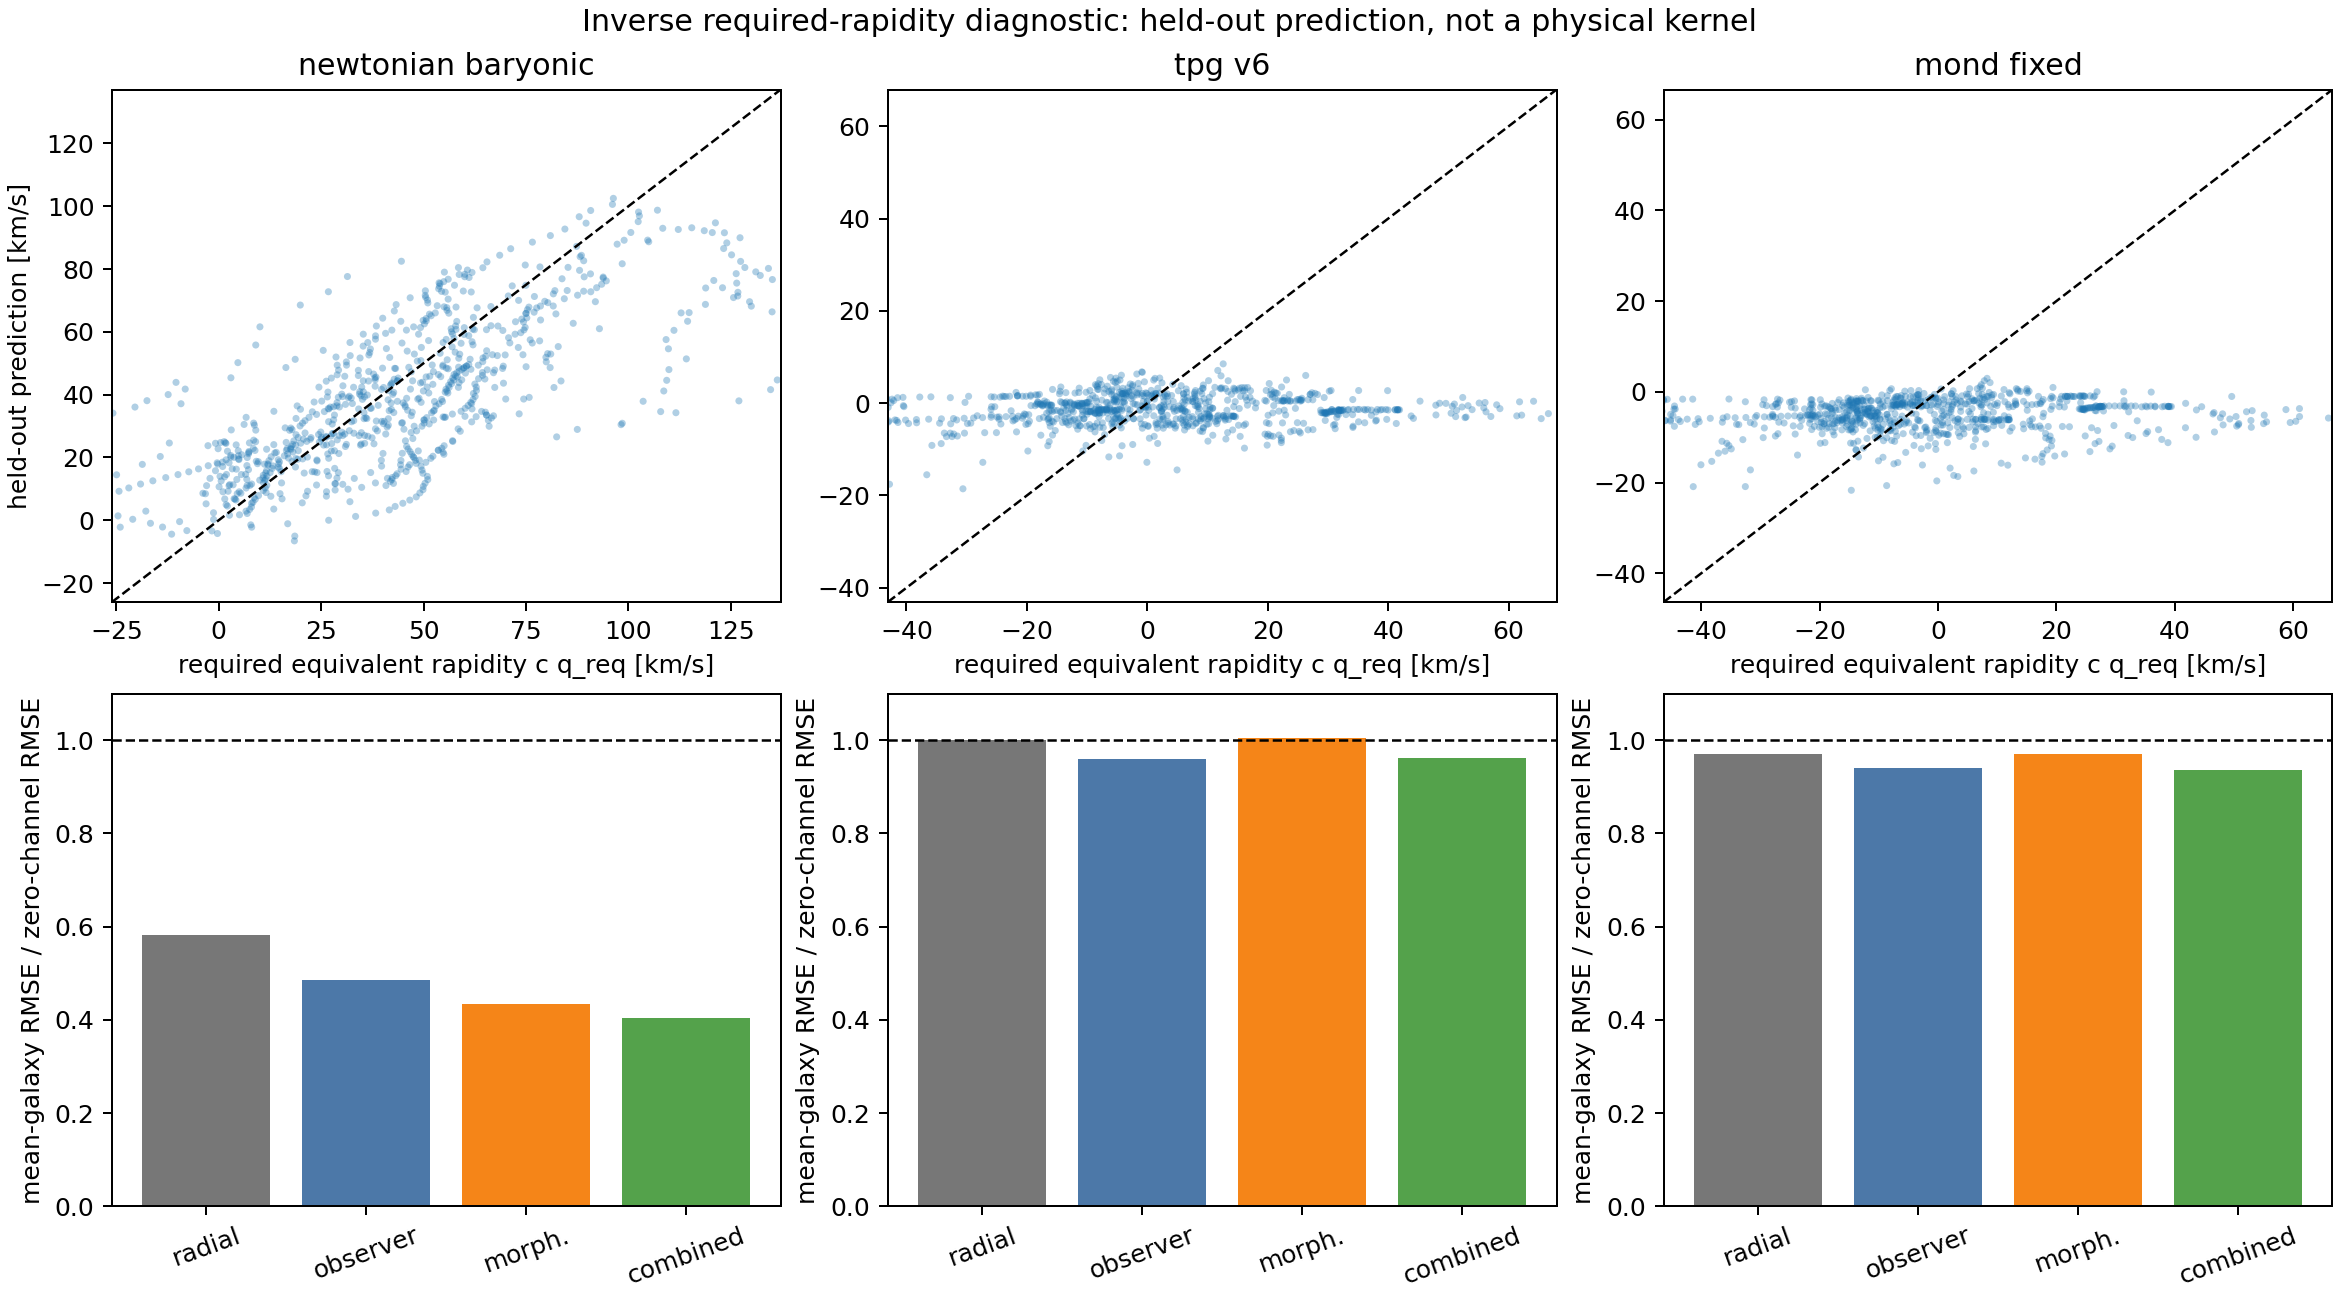
\includegraphics[width=\textwidth]{figures/fig_inverse_required_rapidity_diagnostic_v01.png}
\caption{Held-out inverse required-rapidity diagnostic.  Top: reconstructed
versus combined-model prediction.  Bottom: mean-galaxy RMSE relative to the
zero-additional-rapidity control.  The strong Newtonian result and weak
post-TPG/MOND results have different interpretations; none identifies a
physical Tau source.}
\label{fig:inverse-required-rapidity}
\end{figure}

The informative outcome is therefore primarily negative.  The present broad
source and distance descriptors do not recover a stable universal
post-TPG/MOND rapidity profile on unseen galaxies.  The exercise narrows the
future source search, but it does not derive \(D_O(R)\), a stable \(Q_{OS}\),
body-versus-observer attribution, Nature occupation or a dark-matter
replacement law.

\subsection{Measurement-inverse required parent-loss target}

We also reverse the empirical calculation in the simpler one-parameter shell
\begin{equation}
 v_{\rm obs}^{2}(R)=\frac{v_{\rm base}^{2}(R)}{1-\ell_{\rm req}(R)}.
 \label{eq:inverse-required-parent-loss-shell}
\end{equation}
For positive measured and baseline speeds its exact inverse is
\begin{equation}
 g_{\rm req}=\frac{v_{\rm obs}}{v_{\rm base}},\qquad
 \kappa_{\rm req}=\log g_{\rm req},\qquad
 \ell_{\rm req}=1-\frac{v_{\rm base}^{2}}{v_{\rm obs}^{2}}.
 \label{eq:inverse-required-parent-loss}
\end{equation}
The scalar is unique inside this declared shell, as follows by direct
substitution and injectivity on the positive-speed domain.  Its physical
factorization is not unique.  For example,
\begin{equation}
 \kappa_{\rm req}=\kappa_D-\kappa_T+\kappa_M+\kappa_{\rm cal}
 \label{eq:inverse-required-parent-loss-null}
\end{equation}
maps four pointwise components to one observable and therefore has a
three-dimensional null family.  One rotation terminal cannot attribute the
reconstructed value separately to parent access/distance, temporal
calibration, morphology, or remaining terminal calibration.

Table~\ref{tab:inverse-parent-loss} gives the SPARC reconstruction.  The fixed
cubic profile is trained on the 131 development galaxies and evaluated on the
untouched 44-galaxy holdout; a ratio below one improves on zero required
log-gain.

\begin{table}[htbp]
\centering
\caption{Measurement-inverse required parent-loss diagnostic over 3,389
points in 175 SPARC galaxies.  These values are target reconstructions, not
physical parent-loss estimates or endpoint scores.}
\label{tab:inverse-parent-loss}
\begin{tabular}{lrrrr}
\hline
Baseline & Median gain & Median $\kappa_{\rm req}$ & Median $\ell_{\rm req}$ & Holdout ratio\\
\hline
Newtonian baryonic & 1.6576 & 0.5054 & 0.6360 & 0.5633\\
TPG/v6 & 1.0106 & 0.0105 & 0.0209 & 0.9943\\
fixed MOND & 0.9755 & -0.0248 & -0.0509 & 0.9655\\
\hline
\end{tabular}
\end{table}

The baryonic inversion recodes the familiar mass discrepancy.  After TPG/v6
or MOND, however, the inferred field is sign-mixed and one universal
radius-only cubic profile gives little or no held-out gain.  This rejects that
simple scalar profile inside the declared shell, but it does not reject a
morphology-, channel-, tracer-, or context-conditioned operator.  Baseline
incompleteness, mass-to-light uncertainty, non-circular motions,
inclination/deprojection error, and distance systematics remain direct
conventional alternatives.  The output is therefore an inverse target atlas
for a future source-frozen forward test, not an identification of
$M_\tau$, Nature occupation, or a dark-matter replacement law.

% BEGIN OBSERVER UPDATE 20260914
\section{Observer realization: inherited results and physical boundary}
\label{sec:observer-update-20260914}
The current observer programme distinguishes a conditional mathematical
construction from an occupied physical measuring system. The source order
remains base plus one universal seed, stabilized morphological response,
observer--source restriction, shared descriptor, and resolved terminal
readouts. Neither a detector nor an empirical residual constructs the parent
body backwards. Dynamics below concern downstream subsystems only.

The canonical observer-origin derivation, Sections 22--26, owns the following
results. The existing joint source action fixes static and frequency-dependent
response together. Variation of the BRAC potential couples to the field
square; a linear field coupling is a distinct comparator unless derived by
expansion about an occupied background. Fixed canonical means select a unique
coherent state in a finite positive harmonic packet only if there is no excess
fluctuation energy. This is a free/asymptotic preparation statement, not the
ground state of an interacting detector. For the existing coupled harmonic
pair, the joint ground is pure but either local subsystem is mixed, with its
covariance fixed by the complete joint Hamiltonian.

These are conditional derivations and internal numerical checks. The actual
observer--source context, physical preparation process, kinetic/energy
calibration and stable operational resolution remain unproved. The existing
ORA-T1 selector conditionally chooses stable quantizers when the occupied
context, admissible partition family and positive closure barrier are supplied;
it does not establish those physical premises. A computed ground state is not
a preparation mechanism, and a covariance or optimal abstract measurement is
not an implemented stable quantizer $Q_{OS}$.

\paragraph{Ownership and use.}
The central observer-origin note owns the new contact, state and covariance
derivations; the body-readout technical companion carries the consolidated
mathematics. Foundation Papers IV, V and VI retain physical-selection,
clock-descent and quantum-readout ownership, respectively. This paper imports
only the consequences within its scope. No observational dataset, baseline,
frozen coefficient, score or empirical conclusion is revised by this update.
The reproducibility supplement records the source hashes and the exact
conditional/physical distinction.


\paragraph{Consequence for this paper.}
For galactic inference, these observer constructions do not derive a rotation-curve correction or identify a measured residual as a parent effect. Existing endpoint freezes and scores are unchanged.
% END OBSERVER UPDATE 20260914

% BEGIN LAB UPDATE 20260915
\section{Finite source-to-readout implementation and its scope}
The current finite laboratory is a reproducible implementation, not a new Nature-selection theorem. The modular family search ranks source-side finite conditioning, not galaxy residuals. The separate galaxy-training mode retains an explicitly supplied spectral-log terminal completion; previously exposed or training galaxies are not fresh validation systems. Neither improving a training curve nor changing graph size establishes morphology ownership, a dark-sector explanation or a Tau-specific residual. Published endpoint rules and scores are unchanged.
\paragraph{Ownership and reproducibility.}
The seed--body companion owns the finite minimum/Hessian example, the body--readout companion its ordered access and contact reduction, and the terminal companion its conditional propagation boundary. The physical-source papers retain the source-selection obligation. Code, declared priors, adverse controls and provenance are available at \url{https://github.com/tau-core-research/tau-core-theory/tree/main/experiments/seed_evolution_lab}. Numerical tests are internal evidence only; no published empirical score is changed.
% END LAB UPDATE 20260915

\section{Conclusion}

This paper reframes morphology-sensitive rotation-curve work as a forward
readout problem.  The central claim is not that a new gravity theory has been
validated, nor that every galaxy can be rescued by a custom curve.  The claim is
that a residual-blind morphology/readout state can be used to choose a
predeclared readout family, and that this choice can be tested against wrong
families, shuffled labels, and conventional baselines.

The current numerical evidence is preliminary but useful.  The strongest broad
internal signal is matched label--formula compatibility: source-native readout formulas beat wrong
formula families in \(0.886\) of 44 holdout galaxies with a shuffled-label
\(p\simeq0.002\) for the mean matched-minus-wrong statistic; the
beat-fraction null is reported separately.  The same formulas do not yet beat
TPG/v6 or MOND-like comparators as a population.  Four inspected galaxies are
retained here only as caveated demonstrations of the endpoint workflow.  The
unchanged NGC4088-class transfer to UGC08490 adds an important counterweight:
the correct source onset weakly beats wrong morphology controls, but the full
curve is decisively worse than fixed MOND and standard fit-aided halo models.
The second replication on UGC03580 then removes the remaining universality
claim: the source-correct onset is worse than Newtonian, fixed MOND and earlier
wrong-onset controls, while the uncapped continuation overshoots beyond
\(R_{\rm HI}\).  Hence morphology can carry radial information without the
present one-component warp law being a complete or universal rotation law.
The endpoint-blind radial reconstruction subsequently replaces the onset-only
proxy by a source-complete orientation path on \(S^2\) and reproduces the
published inner/outer plane angle.  This strengthens the morphology
representation but supplies no terminal law and therefore does not alter the
negative endpoint verdict.  A bounded defect-ratio coordinate can be derived
from the two planes, but the explicit
\(v_{p,a,s}^2=v_{\rm c}^2(1+s aK_p)\) counterfamily proves that the same body
admits inequivalent terminal powers, amplitudes, signs, and carriers.  The
standard fixed-inclination control spans \(0.99409\)--\(1.09685\) in squared
speed and must be audited before attributing any residual structure to Tau.
The common-action pullback reduces these apparent independent freedoms to one
signed-descriptor-to-Parent-invariant registration plus the occupied calibrated
gravity/observer packet, but that registration is not selected by the current
source.  The source geometry narrows its hidden fibre to one exact mirror sign:
the oriented source record and the standard fixed-inclination projection show
that the complete stack is not mirror-even, so the signed triple product must
be retained for this lane.  This does not establish Parent chirality or a
Tau-specific coupling.  Normalized-simplex affinity would then select
\(K_1\) uniquely within that scalar class, but the source path itself revisits
the same \(K_1\) level at terminal-distinct locations.  Hence \(K_1\) is not a
complete shared descriptor.  No alternative signed scalar or physically
multicomponent Parent coupling is yet selected.  Consequently,
any physically occupied bounded two-plane replacement
remains a new source-side hypothesis and may not be repaired on these opened endpoints.  The
more detailed observer/projection-enriched kernel derivation and its
four-object audit are separated into a companion paper, because they define a
new validation programme rather than the headline population endpoint of the
present paper.

Two promotion attempts are now explicitly negative.  On the original
45-galaxy label packet, the projection contrast adds no stable cross-fitted
proper-score improvement beyond the frozen observability/baryonic and
MOND/RAR-common baselines.  On the external EDGE--CALIFA packet, the
seven-galaxy source-frozen matched-tracer test gives
\(\overline D=-0.0587\), exact one-sided \(p=0.6016\), and only four positive
objects.  These results preserve the original descriptive association while
blocking its promotion to conditional projection specificity or external
confirmation.

The theory update sharpens the boundary of that programme.  Present morphology,
observer/path appearance, morphology-history phase, and time/readout
descriptors are source-proxy coordinates of one protected source class.  They
may improve a kernel only when frozen independently or merged into a joint
quotient contribution; the same source evidence may not be counted twice as
separate physical corrections.
The accompanying reproducibility package records this boundary in a
paper-level \texttt{KernelRecord\_tau\^{}S} status audit.  That audit classifies the
population lanes, wrong-family controls, shuffled-label tests, and inspected
single-galaxy examples as diagnostic/control, source-proxy, or endpoint-active
frozen kernels.  It does not promote any Paper 8 object to a validated physical
readout.

The next step is therefore not another round of residual-driven curve repair.
It is a readout morphology catalogue, source-grounding audits for any formula
shell promoted beyond proxy status, an independent survey family replacing the
now-exhausted clean HALOGAS lane, and a predeclared endpoint campaign.  If
the correct source-frozen readout family systematically beats wrong families and
shuffled labels, and then becomes competitive against Newtonian, MOND/RAR, and
TPG-like baselines, the framework will have a meaningful empirical target.  If
source-complete endpoint-grade cases fail, those failures should be retained as
true negative candidates.  The absence of such a case in the present analysis
is a limitation of the current source catalogue, not a positive result.

The new representation theorem sharpens that final decision without weakening
the negative record.  The existing failures constrain the frozen A/C,
low-order, S4G, EDGE and PHANGS representations; they do not establish a
source-complete falsification of the general body.  Any successor must be a
genuinely new endpoint-blind \(\Phi_{k+1}\), not a post-open re-expression of
the same residuals.

\appendix
\section{Readout-family derivation ledger}
\label{app:readout-derivations}

This appendix records the manuscript-level derivations of the readout kernels
used in the present population preflight.  The purpose is not to prove a final
gravity law.  It is to make explicit which part is a definition, which part is
a source ansatz, which part follows from a standard radial readout/closure
calculation, and which part remains an empirical or source-completeness
obligation.

This appendix is theory-motivation scaffolding.  The numerical test in the main
text does not require the reader to accept the full Tau Core bridge ontology.
Operationally, the test only requires residual-blind labels, frozen source
proxies, predeclared readout families, and matched-versus-wrong/shuffled
controls.  The bridge equations below explain why these families are grouped
as readout specializations, but the population statistics can be audited from
the saved artifacts even if the parent theory remains unaccepted.

\noindent\fbox{%
\begin{minipage}{0.94\linewidth}
\textbf{Dependency boundary:} the endpoint statistics do not depend on accepting
Appendix~\ref{app:readout-derivations}.  Appendix~\ref{app:readout-derivations}
only motivates the grouping of the readout families and records the formula
ledger used by the reproducibility package.
\end{minipage}
}

\subsection{Tau Core bridge equation used by the readout families}

The readout families in this manuscript are motivated as reductions of one
common conditional bridge object.  Let \(P_D^\tau\) denote the Tau-side
ordered-disk readout slice and let \(P_N^\tau\) denote the Newtonian/metric
closure-test slice.  Their residual-blind local mismatch is
\[
\delta P_\tau = P_N^\tau-P_D^\tau .
\]
Only the tangent/off-slice part of this mismatch can generate a readout
residual.  Denoting that part by \(\delta P_\tau^\perp\), the first-order
relative generator is
\[
\mathcal M_\tau=[\delta P_\tau^\perp,P_D^\tau] .
\]
The bridge then tests whether this generator moves the ordinary diagonal disk
sector outside the Newtonian, ordinary-disk, and gauge subspace
\[
B_{\rm axis}=N+D_{\rm diag}+G .
\]
The non-absorption map is
\[
\rho_D(\mathcal M_\tau)
 :=
\pi_B\circ \mathcal M_\tau|_{D_{\rm diag}},
\qquad
\pi_B:V_{\rm grav}^\tau\to V_{\rm grav}^\tau/B_{\rm axis}.
\]
The common 4D weak-field readout equation used by the present paper is therefore
\begin{equation}
\boxed{
\delta g_{\rm morph}(x)
=
R^{4D}_{g,x}
\left[
\rho_D(\mathcal M_\tau(x))(Q_D^\tau(x))
\right].
}
\label{eq:tau-bridge-base}
\end{equation}
Here \(Q_D^\tau\) is the morphology-selected ordered-disk trace-free direction.
Equation~\eqref{eq:tau-bridge-base} is the bridge base equation used in this
paper.  It is not a final law of gravity; it is a conditional readout rule:
if the Tau-side slice mismatch is source-defined, survives the quotient, and
has a nonzero 4D weak-field readout, then it contributes an effective
morphological residual.

For the local disk witness used throughout the bridge, let \(S_D^\tau\) be the
in-disk shear-like partner of \(Q_D^\tau\).  If the closure-test slice selects
\[
Q_N^\tau
=
\cos\alpha_\tau\,Q_D^\tau
+
\sin\alpha_\tau\,S_D^\tau ,
\]
then, to first order in the local mismatch angle,
\[
\mathcal M_\tau=\alpha_\tau J_D,
\qquad
J_D(Q_D^\tau)=S_D^\tau,
\qquad
J_D(S_D^\tau)=-Q_D^\tau .
\]
Consequently
\begin{equation}
\rho_D(\mathcal M_\tau)(Q_D^\tau)
=
\alpha_\tau [S_D^\tau].
\label{eq:alpha-shear-quotient}
\end{equation}
Equation~\eqref{eq:alpha-shear-quotient} is the algebraic bridge reduction.
It says that the residual is not produced by inserting a new force; it is the
quotient-visible part of a readout/closure mismatch.  The residual vanishes if
\(\alpha_\tau=0\), if \(S_D^\tau\) is absorbed into \(B_{\rm axis}\), or if the
4D readout map kills this quotient class.

\subsection{From bridge residual to a radial family kernel}

To compare with one-dimensional rotation curves, the bridge readout must be
reduced to a radial observable.  In the present preparation-level tests the
family label \(K\) chooses a residual-blind source functional
\(\mathcal S_K^\tau\) representing the observable part of
\(\alpha_\tau[S_D^\tau]\) for that morphology/readout class:
\[
\alpha_\tau [S_D^\tau]
\quad\longrightarrow\quad
\mathcal S_K^\tau .
\]
The 4D readout map then induces a radial operator \(\mathcal R_K\),
\[
\delta g_{K,R}(R)
=
\mathcal R_K[\mathcal S_K^\tau](R),
\]
and circular-orbit comparison uses
\begin{equation}
\delta v_K^2(R)=R\,\delta g_{K,R}(R).
\label{eq:radial-velocity-reduction}
\end{equation}
Thus every endpoint shell below has the common form
\[
\delta v_K^2(R)=A_K K_K(R),
\]
where \(K_K(R)\) is the source-selected radial kernel and \(A_K\) is the
allowed source amplitude or frozen amplitude rule.

This is the derivation status used in the paper:
\begin{itemize}[leftmargin=*]
\item The slice-mismatch and quotient equations
\eqref{eq:tau-bridge-base}--\eqref{eq:alpha-shear-quotient} are the
conditional Tau Core bridge scaffold.
\item The choice of \(\mathcal S_K^\tau\) is a residual-blind morphology/readout
source ansatz, not an endpoint fit.
\item A source-frozen ansatz is not yet a full Tau-side source derivation.  To
promote it beyond proxy status, a separate source-grounding gate must show
activation of a Tau-side mode, survival in the null/gauge quotient, stability
under the relevant closure test, and survival under the four-dimensional readout
map.  In schematic form this later gate is
\[
O_i^{4D}=R_i^{4D}\!\left(\Pi_{\rm stab}([A_\tau(u)])\right).
\]
The present paper defines and tests the operational family proxies; it does not
claim to have discharged this source-grounding gate.
\item The radial kernels \(K_K(R)\) follow from applying the chosen radial
readout operator \(\mathcal R_K\) to that source ansatz.
\item The current population preflight does not prove the parent Tau Core
theory or the exact amplitudes \(A_K\).  It tests whether the residual-blind
family specialization carries information by comparing matched families,
wrong families, shuffled labels, and baseline curves.
\end{itemize}

\begin{table}[H]
\centering
\caption{Logical status of the bridge-to-kernel construction.}
\scriptsize
\resizebox{\linewidth}{!}{%
\begin{tabular}{p{0.24\linewidth}p{0.43\linewidth}p{0.23\linewidth}}
\toprule
Layer & Equation or object & Status in this manuscript\\
\midrule
Tau-side slice mismatch &
\(\delta P_\tau=P_N^\tau-P_D^\tau\),
\(\mathcal M_\tau=[\delta P_\tau^\perp,P_D^\tau]\) &
Definition within the conditional bridge scaffold.\\
Quotient non-absorption &
\(\rho_D=\pi_B\circ\mathcal M_\tau|_{D_{\rm diag}}\),
\(\rho_D(\mathcal M_\tau)(Q_D^\tau)=\alpha_\tau[S_D^\tau]\) &
Conditional algebraic bridge result.\\
4D readout shell &
\(\delta g_{\rm morph}=R_g^{4D}[\rho_D(\mathcal M_\tau)(Q_D^\tau)]\) &
Bridge base equation tested operationally here.\\
Family source specialization &
\(\alpha_\tau[S_D^\tau]\to\mathcal S_K^\tau\) &
Residual-blind source ansatz, family by family.\\
Radial endpoint kernel &
\(\delta v_K^2=R\,\mathcal R_K[\mathcal S_K^\tau]=A_KK_K(R)\) &
Derived shell after choosing the source class and radial readout operator.\\
Amplitude and source completeness &
\(A_K\), source radii, thickness, support, projection state &
Frozen, train-split, or proxy-level depending on the endpoint row.\\
\bottomrule
\end{tabular}
}
\label{tab:bridge-layer-status}
\end{table}

\subsection{Common normalization and dimensional rule}

For every family \(K\), the executable preflight uses a velocity-squared
readout of the form
\[
v_{gK}^2(R)=v_{\rm base}^2(R)+\delta v_{gK}^2(R),
\qquad
\delta v_{gK}^2(R)=A_{gK}K_{gK}(R).
\]
Here \(K_{gK}(R)\) is the source-selected radial kernel and \(A_{gK}\) is the
corresponding amplitude.  The kernel need not be dimensionless.  The
dimensional requirement is simply
\[
[A_{gK}]\,[K_{gK}]=({\rm velocity})^2 .
\]
In a strict endpoint, \(A_{gK}\) must be source-derived or frozen by a
predeclared rule.  In the current population preflight, the family shapes are
the derived readout shells, while several source scales and amplitudes remain
available-data proxies or train-split normalizations.  That is why the
population result is an internal label--formula compatibility signal, not a
conditional or externally replicated morphology-specific result and not a final
empirical validation.

\subsection{Scale-tail or diffuse LSB readout}

\paragraph{Definition/source ansatz.}
The scale-tail family is used when the source morphology indicates an extended
outer load, diffuse low-surface-brightness support, or an H I/tail-like
readout component.  The residual-blind source inputs are an inner onset radius
\(R_{\rm in}\) and an outer cutoff/support radius \(R_{\rm cut}\).  The minimal
\(n=2\) tail window is
\[
W_{\rm tail}(r)
=
\frac{(r/R_{\rm in})^2}{1+(r/R_{\rm in})^2}
\frac{1}{1+(r/R_{\rm cut})^2}.
\]
The first factor suppresses the inner disk; the second keeps the source
finite.

\paragraph{Bridge specialization.}
In Eq.~\eqref{eq:tau-bridge-base}, the scale-tail family corresponds to a
source class \(\mathcal S_{\rm tail}^\tau=A_{\rm tail}W_{\rm tail}(r)\) whose
quotient-visible readout is dominated by an extended outer support.  The radial
operator \(\mathcal R_{\rm tail}\) is the one-dimensional accumulated-load
readout.  Thus the family is obtained by applying
\(\delta v^2=R\,\mathcal R_{\rm tail}[\mathcal S_{\rm tail}^\tau]\), not by
fitting an arbitrary tail shape to the rotation residual.

\paragraph{Radial readout.}
For a one-dimensional preflight, the allowed radial load is the accumulated
tail source
\[
I_2(R)=\int_0^R W_{\rm tail}(r)\,dr .
\]
The corresponding scale-tail velocity-squared response is taken to be
\[
\boxed{
\delta v_{\rm tail}^2(R)
=
A_{\rm tail}\frac{I_2(R)}{R}
}
\qquad
K_{\rm tail}(R)=I_2(R)/R .
\]
This is the formula implemented in the reproducibility code as the
\(n=2\) scale-tail shell.

\paragraph{Limits.}
For \(R\ll R_{\rm in}\), \(W_{\rm tail}\sim (R/R_{\rm in})^2\), so the tail
readout is suppressed in the inner disk.  For
\(R_{\rm in}\ll R\ll R_{\rm cut}\), \(I_2(R)\sim R\), so
\(I_2(R)/R\) approaches a slowly varying or flat contribution.  For
\(R\gg R_{\rm cut}\), \(I_2(R)\) saturates and the response falls as \(1/R\) in
velocity squared.  Thus the shell has the intended inner-suppressed,
outer-supported, finite-tail behavior without reading endpoint residuals.

\paragraph{Claim boundary.}
This derivation fixes the readout shape once \(R_{\rm in}\) and
\(R_{\rm cut}\) are source-frozen.  It does not by itself derive the amplitude
\(A_{\rm tail}\), nor does it prove that every diffuse or LSB galaxy belongs to
this family.

\subsection{Regular exponential-disk readout}

\paragraph{Definition/source ansatz.}
The exponential-disk family is used when the source morphology is a regular
axisymmetric disk with a residual-blind scale radius \(R_s\).  The source
surface readout is
\[
\Sigma_{\rm exp}(R)=\Sigma_0 e^{-R/R_s}.
\]

\paragraph{Bridge specialization.}
In the bridge notation, this family chooses
\(\mathcal S_{\rm exp}^\tau=A_{\rm exp}\Sigma_0 e^{-R/R_s}\) as a regular
axisymmetric source class.  The corresponding radial operator
\(\mathcal R_{\rm exp}\) is the standard axisymmetric disk Green operator.  It
is included as a conservative bridge specialization: the Tau-side family
selection decides when the regular-disk carrier is the appropriate readout,
while the carrier itself is the familiar exponential-disk radial response.

\paragraph{Radial readout.}
The axisymmetric thin-disk Green-function calculation for an exponential disk
gives the standard Freeman radial carrier \cite{Freeman1970Disk}
\[
v_{\rm exp}^2(R)
\propto
y^2\left[I_0(y)K_0(y)-I_1(y)K_1(y)\right],
\qquad
y=\frac{R}{2R_s},
\]
where \(I_n\) and \(K_n\) are modified Bessel functions.  The preflight kernel
keeps this source-fixed shape and absorbs dimensional constants into the
amplitude:
\[
\boxed{
\delta v_{\rm exp}^2(R)
=
A_{\rm exp}\,
R_s\,y^2\left[I_0(y)K_0(y)-I_1(y)K_1(y)\right]
}
\]
or
\[
K_{\rm exp}(R)=
R_s\,y^2\left[I_0(y)K_0(y)-I_1(y)K_1(y)\right].
\]

\paragraph{Limits.}
The response is finite at the origin, peaks on disk scales, and declines at
large radii.  It is therefore a regular-disk carrier, not an arbitrary
long-range tail.

\paragraph{Claim boundary.}
This is the most conservative readout family: it imports the standard
axisymmetric exponential-disk radial carrier as the morphology-matched shell.
The current paper does not claim that this is a new gravity formula.  It tests
whether source morphology can decide when this restricted shell is the right
readout family.

\subsection{Compact finite-source readout}

\paragraph{Definition/source ansatz.}
The compact family is used when the source morphology indicates centrally
concentrated or finite support with an outer compact radius \(R_c\).  The
minimal assumption is that the active readout load is finite:
\[
I_{\rm compact}(R)\longrightarrow I_\infty
\qquad (R>R_c).
\]

\paragraph{Bridge specialization.}
Here \(\mathcal S_{\rm compact}^\tau\) is the finite-support quotient-visible
source class produced by Eq.~\eqref{eq:tau-bridge-base}.  The radial readout
operator \(\mathcal R_{\rm compact}\) is used only in its exterior finite-load
limit unless stronger source information is available.  Therefore the
\(1/R\) velocity-squared shell is a compact-source consequence, while the
inner continuation used by the code is a numerical regularization.

\paragraph{Exterior readout.}
Outside the support, any finite radial load has the leading exterior behavior
\[
\delta g_R(R)\sim -\frac{B_c}{R^2},
\]
and therefore
\[
\boxed{
\delta v_{\rm compact}^2(R)=R\,|\delta g_R(R)|
\sim
\frac{B_c}{R}
}
\qquad (R\ge R_c).
\]
The executable preflight uses
\[
K_{\rm compact}(R)=
\begin{cases}
R^2/R_c^3, & R<R_c,\\
1/R, & R\ge R_c,
\end{cases}
\]
so that the kernel is finite in the inner numerical domain and matches the
exterior \(1/R\) value at \(R=R_c\).

\paragraph{Limits.}
The scientifically meaningful part of this shell is the exterior finite-load
falloff.  The inner regularization is a numerical preflight convention, not a
claim about the detailed central dynamics.

\paragraph{Claim boundary.}
This family is endpoint-ready only when \(R_c\) is source-native or frozen
residual-blind.  A compact label without a compact-support source field is a
candidate or control, not a validation row.

\subsection{Thick/flared or projection-sensitive readout}

\paragraph{Definition/source ansatz.}
The thick/flared family is used when the source morphology indicates vertical
support, flaring, edge-on projection, or projection-sensitive readout.  The
source inputs are a disk scale \(R_s\) and a dimensionless thickness profile
\(h(R)/R_s\), or a frozen constant proxy when no radial profile is available.

\paragraph{Bridge specialization.}
For this family, Eq.~\eqref{eq:tau-bridge-base} is reduced with a
three-dimensional/projection-sensitive source class
\(\mathcal S_{\rm flare}^\tau(R,z)\).  In a one-dimensional SPARC preflight,
the vertical part cannot be fully resolved, so its effect enters the radial
operator \(\mathcal R_{\rm flare}\) as a damping of short-wavelength Hankel
modes.  This is why the shell is a projection/readout attenuation, not a
generic extra force.

\paragraph{Damped Fourier-Bessel readout.}
The thin exponential-disk response can be written as a Hankel/Fourier-Bessel
radial integral.  Vertical thickness damps high spatial-frequency modes.  The
minimal constant-\(h\) damping used in the preflight is
\[
D(u,h/R_s)=\frac{1}{1+u\,h/R_s}.
\]
With \(x=R/R_s\), the thick/flared shell is
\[
\boxed{
K_{\rm flare}(R)
=
R_s\,\frac{x}{2}
\int_0^\infty
\frac{u\,J_1(ux)}{(1+u^2)^{3/2}}
\frac{du}{1+u\,h/R_s}
}
\]
and
\[
\delta v_{\rm flare}^2(R)=A_{\rm flare}K_{\rm flare}(R).
\]

\paragraph{Limits.}
When \(h/R_s\to 0\), the damping tends to unity and the shell reduces to the
thin-disk radial carrier class.  Larger \(h/R_s\) suppresses short-wavelength
radial structure and gives a smoother projected response.  This is the desired
behavior for vertical/projection-sensitive systems.

\paragraph{Claim boundary.}
The current SPARC population run mostly uses scalar thickness proxies, so this
family is a one-dimensional proxy for a genuinely three-dimensional readout.
It becomes endpoint-grade only when vertical/projection observables are
source-frozen strongly enough.

\subsection{Ring, barred, and lopsided families}

The registry also contains ring/resonance, barred \(m=2\), and lopsided \(m=1\)
families.  Their source forms are
\[
\Sigma_{\rm ring}(R)\propto
\exp\!\left[-\frac{(R-R_{\rm ring})^2}{2w_{\rm ring}^2}\right],
\]
and
\[
\Sigma_m(R,\phi)=\Sigma_m(R)\cos[m(\phi-\phi_m)],
\qquad m=1,2 .
\]
These are legitimate morphology handles, but they are not promoted here to
full one-dimensional endpoint kernels.  The ring family can sometimes be used
as a localized radial proxy if \(R_{\rm ring}\) and \(w_{\rm ring}\) are
source-frozen.  The \(m=1\) and \(m=2\) families are intrinsically
velocity-field objects because their phase information is largely lost in a
one-dimensional azimuthally averaged rotation curve.  Treating them as full
SPARC-1D endpoint families would overstate the evidence.

\subsection{Summary of derivation status}

\begin{table}[H]
\centering
\caption{Readout-family derivation status.  ``Derived shell'' means that the
kernel shape follows from the stated source ansatz and radial readout
calculation.  It does not mean that the amplitude or source classification is
empirically validated.}
\scriptsize
\resizebox{\linewidth}{!}{%
\begin{tabular}{p{0.18\linewidth}p{0.30\linewidth}p{0.24\linewidth}p{0.18\linewidth}}
\toprule
Family & Derived kernel & Required source freeze & Status in this paper\\
\midrule
\(K_{\rm scale\_tail\_spiral}\) &
\(K_{\rm tail}=I_2(R)/R\), \(I_2=\int_0^R W_{\rm tail}(r)dr\) &
\(R_{\rm in}\), \(R_{\rm cut}\), amplitude policy &
Derived 1D shell; source scales often proxy.\\
\(K_{\rm exponential\_disk}\) &
\(K_{\rm exp}=R_s y^2[I_0K_0-I_1K_1]\) &
\(R_s\), amplitude policy &
Derived standard disk carrier; conservative 1D shell.\\
\(K_{\rm compact\_finite}\) &
\(K_{\rm compact}\sim 1/R\) outside \(R_c\) &
\(R_c\), finite-load evidence, amplitude policy &
Exterior shell derived; inner regularizer is numerical.\\
\(K_{\rm thick\_flared}\) &
damped Fourier-Bessel kernel with \(D=(1+u h/R_s)^{-1}\) &
\(R_s\), \(h/R_s\) or profile, projection state &
Derived 1D proxy for 3D/projection readout.\\
\(K_{\rm ring}\) &
localized radial source convolution near \(R_{\rm ring}\) &
\(R_{\rm ring}\), \(w_{\rm ring}\), phase/context &
Proxy only in this paper.\\
\(K_{m=1},K_{m=2}\) &
harmonic velocity-field response &
\(\Sigma_m(R)\), phase \(\phi_m\), velocity field &
Velocity-field preferred; not a full 1D endpoint kernel.\\
\bottomrule
\end{tabular}
}
\end{table}

\section{Holdout per-galaxy freeze ledger}
\label{app:holdout-ledger}

Table~\ref{tab:holdout-ledger} is an abbreviated ledger for the 44 holdout
galaxies behind the \(0.886\) source-native formula result.  The full machine
ledger is \path{data/derived/source_native_readout_formula_labels.csv}; the
score ledger is \path{data/derived/source_native_readout_formula_scores_by_galaxy.csv}.
The source-proxy vector is reported as
\[
R_s/R_{\rm in}/R_{\rm cut}/R_c/(h/R_s).
\]
These are not claimed to be final source-native observables; they are the
frozen available-data proxies used by the executable preflight.  Caveat codes:
FPTS = few rotation points, LINC = low inclination, LDE = large distance error,
and VPROXY = vertical geometry proxy only.  The final column reports
matched-minus-wrong-family mean RMSE, so negative \(\Delta\) means the matched
family beats the wrong-family mean.

\begin{landscape}
\begingroup
\small
\setlength{\tabcolsep}{3pt}
\begin{longtable}{@{}p{0.105\linewidth}p{0.070\linewidth}p{0.060\linewidth}p{0.085\linewidth}p{0.130\linewidth}p{0.280\linewidth}p{0.120\linewidth}@{}}
\caption{Abbreviated holdout per-galaxy label/source/score ledger.}
\label{tab:holdout-ledger}\\
\toprule
Galaxy & Family & Conf. & Role & Caveat & Source vector & Outcome\\
\midrule
\endfirsthead
\toprule
Galaxy & Family & Conf. & Role & Caveat & Source vector & Outcome\\
\midrule
\endhead
\midrule
\multicolumn{7}{r}{Continued on next page}\\
\midrule
\endfoot
\bottomrule
\endlastfoot
CamB & tail & 1.00 & middle & none & 0.54/0.32/2.09/0.90/0.23 & win; $-71.52$ \\
ESO116-G012 & exp & 0.85 & middle & LDE & 2.46/1.45/10.95/4.13/0.18 & win; $-10.25$ \\
F561-1 & tail & 0.60 & candidate & FPTS,LINC & 3.36/1.98/10.89/5.64/0.19 & win; $-13.86$ \\
F563-1 & tail & 0.65 & candidate & LINC,LDE & 5.52/3.24/24.89/9.26/0.29 & win; $-2.90$ \\
F568-1 & flare & 0.70 & candidate & LINC,VPROXY & 3.09/1.81/14.68/5.19/0.18 & loss; $5.40$ \\
IC2574 & tail & 1.00 & control & none & 3.30/1.94/12.16/5.54/0.25 & win; $-16.19$ \\
IC4202 & compact & 1.00 & candidate & none & 7.69/4.52/26.52/18.33/0.10 & win; $-0.43$ \\
NGC0024 & flare & 0.90 & middle & VPROXY & 1.01/0.59/11.84/1.70/0.13 & win; $-26.51$ \\
NGC2683 & flare & 0.90 & middle & VPROXY & 10.32/6.06/35.26/18.95/0.10 & win; $-2.99$ \\
NGC3726 & flare & 0.90 & candidate & VPROXY & 7.79/4.57/34.51/13.06/0.14 & win; $-4.36$ \\
NGC3949 & flare & 0.70 & middle & FPTS,VPROXY & 2.60/1.53/7.29/4.37/0.11 & win; $-14.09$ \\
NGC3972 & flare & 0.90 & middle & VPROXY & 2.86/1.68/9.07/4.80/0.12 & win; $-11.38$ \\
NGC4013 & compact & 1.00 & middle & none & 10.86/6.38/32.08/22.26/0.11 & loss; $5.33$ \\
NGC4088 & flare & 0.90 & candidate & VPROXY & 6.75/3.97/22.44/11.33/0.12 & win; $-4.72$ \\
NGC4183 & exp & 1.00 & control & none & 6.24/3.66/24.28/10.47/0.22 & win; $-7.54$ \\
NGC4214 & tail & 0.80 & middle & LINC & 1.74/1.02/6.14/2.92/0.16 & win; $-23.65$ \\
NGC4389 & flare & 0.70 & candidate & FPTS,VPROXY & 1.87/1.10/5.38/3.15/0.09 & win; $-21.07$ \\
NGC5907 & flare & 0.90 & middle & VPROXY & 16.50/9.69/54.29/27.68/0.15 & win; $-1.22$ \\
NGC5985 & compact & 0.85 & candidate & LDE & 9.32/5.47/35.23/17.80/0.09 & win; $-7.42$ \\
NGC6789 & tail & 0.80 & middle & FPTS & 0.24/0.14/0.82/0.41/0.22 & win; $-107.71$ \\
NGC6946 & compact & 0.65 & middle & LINC,LDE & 6.13/3.60/21.14/11.86/0.11 & loss; $13.68$ \\
NGC7331 & flare & 0.90 & candidate & VPROXY & 10.49/6.16/37.61/18.84/0.11 & win; $-1.84$ \\
UGC00731 & tail & 0.85 & middle & LDE & 3.52/2.07/14.72/5.91/0.39 & win; $-16.98$ \\
UGC00891 & tail & 0.65 & control & FPTS,LDE & 2.65/1.56/9.79/4.45/0.37 & win; $-23.48$ \\
UGC02023 & tail & 0.45 & middle & FPTS,LINC,LDE & 1.35/0.79/4.17/2.27/0.17 & win; $-37.05$ \\
UGC02259 & exp & 0.85 & middle & LDE & 2.73/1.60/9.43/4.58/0.22 & win; $-8.92$ \\
UGC03580 & compact & 0.85 & candidate & LDE & 1.64/0.96/28.70/4.07/0.13 & loss; $28.48$ \\
UGC04305 & tail & 1.00 & candidate & none & 1.72/1.01/6.42/2.88/0.23 & win; $-28.17$ \\
UGC04499 & tail & 0.85 & control & LDE & 2.71/1.59/9.82/4.55/0.26 & win; $-18.61$ \\
UGC05414 & tail & 0.65 & control & FPTS,LDE & 1.43/0.84/4.78/2.40/0.23 & win; $-33.83$ \\
UGC05716 & tail & 0.85 & control & LDE & 4.00/2.35/16.03/6.71/0.35 & win; $-17.56$ \\
UGC05829 & tail & 0.65 & control & LINC,LDE & 2.25/1.32/8.32/3.77/0.26 & win; $-25.96$ \\
UGC05986 & tail & 0.85 & middle & LDE & 2.99/1.76/10.17/5.02/0.15 & win; $-9.47$ \\
UGC06818 & tail & 1.00 & middle & none & 2.35/1.38/7.62/3.94/0.16 & win; $-21.42$ \\
UGC06917 & tail & 1.00 & control & none & 3.64/2.14/11.44/6.11/0.16 & win; $-14.68$ \\
UGC06983 & tail & 1.00 & middle & none & 5.20/3.05/18.45/8.72/0.24 & win; $-8.10$ \\
UGC07151 & exp & 1.00 & control & none & 1.79/1.05/6.04/3.00/0.17 & win; $-29.87$ \\
UGC07261 & exp & 0.45 & control & FPTS,LINC,LDE & 2.27/1.33/7.36/3.81/0.17 & win; $-22.60$ \\
UGC07577 & tail & 1.00 & middle & none & 0.56/0.33/1.78/0.94/0.13 & win; $-69.53$ \\
UGC07603 & exp & 0.85 & middle & LDE & 1.32/0.78/4.80/2.22/0.23 & win; $-32.16$ \\
UGC08699 & compact & 0.85 & middle & LDE & 4.27/2.51/26.33/10.75/0.10 & win; $-2.94$ \\
UGC11914 & compact & 0.65 & candidate & LINC,LDE & 2.28/1.34/9.85/6.01/0.08 & win; $-10.70$ \\
UGC12506 & exp & 1.00 & candidate & none & 15.14/8.89/55.56/25.41/0.18 & loss; $4.99$ \\
UGCA444 & tail & 1.00 & control & none & 0.81/0.48/3.74/1.36/0.47 & win; $-54.28$ \\
\end{longtable}
\endgroup
\end{landscape}

\section{Source-reference ledger}

Table~\ref{tab:source-ledger} records how the main external references enter the
present paper.  The entries are provenance for residual-blind source fields and
baseline context.  They do not by themselves validate any readout formula.

\begin{table}[H]
\centering
\caption{Reference ledger for source fields used or proposed by the
morphology-readout protocol.}
\label{tab:source-ledger}
\scriptsize
\resizebox{\linewidth}{!}{%
\begin{tabular}{p{0.18\linewidth}p{0.31\linewidth}p{0.38\linewidth}}
\toprule
Reference group & Role in this paper & Claim boundary\\
\midrule
\cite{Lelli2016SPARC} &
SPARC rotation curves and baryonic mass-model arena. &
Common numerical data source; not a readout-morphology catalogue.\\
\cite{Milgrom1983MOND,McGaugh2016RAR,Li2018RARFits} &
MOND-like and empirical RAR comparison context. &
Baseline comparators; not used to choose morphology-readout families.\\
\cite{Freeman1970Disk} &
Standard exponential-disk radial carrier used in the regular-disk readout
derivation. &
Formula-context reference; not evidence for the morphology-matched endpoint
protocol by itself.\\
\cite{Trachternach2008THINGS,VerheijenSancisi2001UrsaMajorHI,Spekkens2006RapidRotators,vanEymeren2011WHISPLopsidedness} &
Examples of H I, velocity-field, late-type photometric/kinematic, and
lopsidedness data products suitable for readout morphology fields. &
Support feasibility of a catalogue; object-specific endpoint gates still require
per-galaxy source freeze.\\
\cite{NED,Sheth2010S4G,Davies2017DustPedia,Leroy2021PHANGSALMA} &
Catalogue, decomposition, multiwavelength, and resolved-gas infrastructure
needed for a residual-blind readout morphology catalogue. &
Source-infrastructure references; they support data availability and provenance,
not endpoint validation by themselves.\\
\cite{Levy2018EDGECALIFAKinematics,Wong2023EDGEData} &
Matched-resolution EDGE CO and CALIFA optical maps, velocity-convention
calibration, and the external seven-galaxy confirmation packet. &
The frozen morphology-alignment proxy fails its promotion gate; the data source
does not identify a Tau mechanism or exhaust standard astrophysics.\\
\cite{Begeman1989NGC3198HI,Gentile2013HALOGASNGC3198,Schmidt2016THINGSRadialGas} &
NGC3198 H I extent, extraplanar gas, and radial-flow/tail-onset source context. &
Used to illustrate source acquisition and failure-mode routing; not promoted as
an accepted endpoint in this paper.\\
\cite{ZschaechnerRand2015NGC4013HI,Comeron2011NGC4013Vertical} &
NGC4013 H I and vertical-structure context. &
Supports mixed/vertical-overlay interpretation; NGC4013 remains retrospective
and replay-needed.\\
\cite{Sasaki1987NGC5907Warp,Shang1998NGC5907Warp,Wiegert2015EdgeOnISM} &
NGC5907 warp, edge-on, and projection/ISM context. &
Supports the projection/mixed readout lane; single-galaxy result remains
preliminary.\\
\cite{Bosma1978NGC7331HI,Patra2018NGC7331ScaleHeight} &
NGC7331 H I warp/history and vertical-scale context. &
Supports caveated mixed endpoint and pure-branch negative-control interpretation.\\
\cite{VerheijenSancisi2001UrsaMajorHI} &
NGC4088 H I geometry, strong disk distortion, position--velocity asymmetry,
asymmetric warp behaviour, and near-companion context. &
Supports the warp/history/asymmetric-projection readout lane; current NGC4088
result remains source-review and normalization-law caveated.\\
\cite{deBlok2020IC2574HI,WalterBrinks1999IC2574Holes,SanchezSalcedo2002IC2574Holes,Swaters2009LateTypeDwarfs} &
Exploratory disturbed/dwarf H I morphology source classes. &
Included as examples for future catalogue lanes; not scored as endpoint evidence
here.\\
\bottomrule
\end{tabular}
}
\end{table}


\bibliographystyle{plain}
\bibliography{refs}
\end{document}
